\documentclass{article}
\usepackage[margin=1.0in]{geometry}
\usepackage{amssymb,amsmath,amsthm,amsfonts,mathtools,systeme}
\usepackage{enumitem}
\usepackage{xcolor}

\newcommand{\Z}{\mathbf{Z}}
\newcommand{\N}{\mathbf{N}}
\newcommand{\R}{\mathbf{R}}
\newcommand{\Q}{\mathbf{Q}}
\newcommand{\C}{\mathbf{C}}
\newcommand{\NA}{\mathbf{N}}

\newcommand{\id}{\mathrm{id}}
\newcommand{\op}{\mathrm{op}}
\newcommand{\diam}{\mathrm{diam}}
\newcommand{\rank}{\mathrm{rank}}
\newcommand{\GL}{\mathrm{GL}}
\newcommand{\Tr}{\mathrm{Tr}}
\newcommand{\vol}{\mathrm{vol}}

\newcommand{\cl}[1]{\overline{#1}}

\swapnumbers % places numbers before thm names

\allowdisplaybreaks

\theoremstyle{plain} % The "plain" style italicizes all body text.
	\newtheorem{thm}{Theorem}
		\numberwithin{thm}{section} % Theorem numbers are determined by section.
	\newtheorem{lemma}[thm]{Lemma}
	\newtheorem{prop}[thm]{Proposition}
	\newtheorem{cor}[thm]{Corollary}

\theoremstyle{definition}
    \newtheorem{defn}[thm]{Definition}
	\newtheorem{example}[thm]{Example}
	\newtheorem{exercise}[thm]{Exercise} %Exercise

\title{MAT257 Final Portfolio}
\author{Ethan Hua}
\date{}

\begin{document}
    \maketitle
    \newpage
    \tableofcontents
    \section{Big List Problems}
    \begin{center}
        \begin{tabular}{ | c | c |}
            \hline
            \textbf{Problem Number} & \textbf{Completed?} \\
            \hline
            \#1 & Complete \\
            \hline
            \#2 & Incomplete \\
            \hline
            \#3 & Complete \\
            \hline
            \#4 & Complete \\
            \hline
            \#5 & Complete \\
            \hline
            \#6 & Complete \\
            \hline
            \#7 & Complete \\
            \hline
            \#8 & Complete \\
            \hline
            \#9 & Complete \\
            \hline
            \#10 & Complete \\
            \hline
            \#11 & Complete \\
            \hline
            \#12 & Complete (Specially Selected) \\
            \hline
            \#13 & Unfinished \\
            \hline
            \#14 & Unattempted \\
            \hline
            \#15 & Unattempted \\
            \hline
            \#16 & Complete (Specially Selected) \\
            \hline
            \#17 & Complete (Specially Selected) \\
            \hline
            \#18 & Complete \\
            \hline
            \#19 & Incomplete \\
            \hline
            \#20 & Complete (Specially Selected) \\
            \hline
            \#21 & Unattempted \\
            \hline
            \#22 & Complete (Specially Selected)\\
            \hline
            \#23 & Complete \\
            \hline
            \#24 & Complete \\
            \hline
            \#25 & Complete \\
            \hline
            \#26 & Complete \\
            \hline
            \#27 & NA \\
            \hline
            \#28 & NA \\
            \hline
            \#29 & NA \\
            \hline
        \end{tabular}
    \end{center}
    \subsection{\#1}

    Let $A_1,A_2,A_3,\ldots$ be a sequence of countable sets. Prove that $\bigcup_{i\geq 1} A_i$ is countable.

    \smallskip

    \noindent My previous submission did not take into account the fact that the sets could have been not disjoint. This resubmission should resolve that issue.


    \noindent\textbf{Changelog:}\begin{enumerate}
        \item Fixed the argument to address the non-disjoint case.
    \end{enumerate}

    \begin{proof}
        \textcolor{red}{Notice that \[\bigcup_{i \ge 1} A_i = A_1 \cup (A_2 \setminus A_1) \cup (A_3 \setminus (A_1 \cap A_2)) \cup \dots\] We define a new collection of sets \(\{B_i\}\) as follows:}
        \textcolor{red}{
            \[
                B_1 = A_1
            \] 
            \[
                B_k = A_k \setminus \left(\bigcap_{i=1}^{k-1} A_i\right) \text{, } k>1
            \]
        }
        Since \(A_i\) is countable, denote \(A_{ij}\) to be the \(j\)th element of set \(A_i\). \textcolor{red}{Noting that \(\bigcup_{i \ge 1} A_i = \bigcup_{i \ge 1} B_i\), Define \(f: \bigcup_{i \ge 1} B_i \to \mathbb{N}\) as }
        \[
            f(A_{ij})=2^{i}3^{j}
        \]
        We will show that \(f\) is injective. Let \(A_{pq}, A_{rs} \in \textcolor{red}{\bigcup_{i \geq 1} B_i}\). Suppose that \(f(A_{pq} ) = f(A_{rs} )\). Then
        \[
            2^p 3^q = 2^r 3^s
        \]
        Since every integer has a unique prime factorisation, it follows that \(p = r\), \(q = s\). Thus \(A_{pq} = A_{rs} \).

        \noindent \\ Now, define the injection \(g: \mathbb{N} \to \bigcup_{i\geq 1} A_i\) to be \(g(n) = A_{1n} \). 
        
        \noindent Therefore by the Schröder–Bernstein theorem, \(|\bigcup_{i\geq 1} A_i | = |\mathbb{N} |\). Thus the set is countable.

    \end{proof}

    \subsection{\#2 - Incomplete}

    This problem is incomplete for a variety of reasons. Firstly, I did not show that \(\phi\) is a linear mapping. Secondly, \(\phi\) is not well-defined because based on the supposed codomain of \(\phi\), \(\phi (T)\) should only take in one input, whereas I defined \(\phi (T)\) by inputting two inputs. Finally, the basis argument I made when showing that \(\phi\) is surjective was unnecessary, and I could have just directly defined \(T(x,y) = U(x)(y)\).

    \bigskip

    Let $X,Y,Z$ be three vector spaces. Prove that $L^2(X,Y;Z)$ is isomorphic to $L(X,L(Y,Z))$.

   (For two vector spaces $X,Y$, we use $L(X,Y)$ to denote the space of linear mappings from $X$ to $Y$. For three vector spaces $X,Y,Z$, and a a function $\beta:X\times Y\rightarrow Z$, we let $\beta(\,\cdot\,,y_0)$ denote the function $X\rightarrow Z$ given by $x\mapsto \beta(x,y_0)$, where $y_0\in Y$ is some fixed vector; this is called the \textbf{$y_0$-slice} of $\beta$. The \textbf{$x_0$-slice} $\beta(x_0, \,\cdot\,)$ is defined similarly.)

   \begin{proof}
        For a bilinear map \(T \in L^2(X,Y;Z)\), \((x,y) \in X \times Y\), Define \(\phi : L^2(X,Y;Z) \to L(X,L(Y,Z))\) such that
        \[
            \phi (T)(x,y) = T(x, \cdot)(y)
        \]  
        where \(T(x,\cdot)\) is the \(x\)-slice of \(T\). We claim that this transformation is an isomorphism.

        First, let \(\phi (T) = 0\). Then \(\forall x \in X \text{,} T(x, \cdot)(y) = 0\), from which it follows that \(T(x, y) = 0\), meaning \(\phi\) is injective. 
        
        Next, fix \(U \in L(X,L(Y,Z))\). Let \(\beta \) be the basis for \(X\). Let \(T \in L^2(X,Y;Z)\) be the linear transformation such that \(T(x, \cdot) = U(x) \text{, for all } x \in \beta \). We see that \(\forall x,y \in X \times Y\),
        \[
            \phi (T)(x,y) = T(x, \cdot)(y) = U(x)(y)
        \]
        making \(\phi \) surjective.

        Thus \(\phi \) is an isomorphism, and we get that \(L^2(X,Y;Z) \cong L(X,L(Y,Z))\) as desired.
   \end{proof}

   \subsection{\#3}

   Let $I=(a,b)$ and $J=(c,d)$ be two open intervals on the real line. Let $f:I\rightarrow J$ be an increasing function such that $f(I)$ is dense in $J$. Prove that $f$ is continuous.

    (For two sets $D,S\subseteq \R$ we say that $D$ is \textbf{dense} in $S$ if $D\cap (s-\varepsilon,s+\varepsilon)\neq\varnothing$ for all $s\in S$ and all $\varepsilon>0$.)
    \begin{proof}
        Fixing an \(a \in I\), let \(\varepsilon > 0\). We can assume without loss of generality that \(\varepsilon \) is small enough that \((f(a) - \varepsilon , f(a) + \varepsilon ) \subseteq J\). Since \(f(I)\) is dense in \(J\), we can always find an \(y_1 \in (f(a) - \varepsilon , f(a)) \text{ and } y_2 \in (f(a), f(a) + \varepsilon )\) such that \(y_1 , y_2 \in f(I)\), which means \(y_1 = f(x_1) \text{ and } y_2 = f(x_2)\) for some \(x_1, x_2 \in I\).

        Take \(\delta = \min \{\lvert a - x_1 \rvert , \lvert a - x_2 \rvert \}\). Let \(x \in I\). Suppose that \(\lvert x - a \rvert\leq \delta \). If \(x = a\), clearly \(\lvert f(x) - f(a) \rvert < \varepsilon \). Consider when \(x < a\).

        We see that due to the choice of \(\delta \), we have that \(x_1 < x < a\). Using the fact that \(f\) is increasing, we obtain
        \[
            f(a) - \varepsilon < y_1 = f(x_1) < f(x) < f(a) \implies - \varepsilon < f(x) - f(a) < 0 \implies f(a) - f(x) = \lvert f(x) - f(a) \rvert < \varepsilon 
        \] 
        The argument for the case when \(x < a\) is almost the exact same, except for the use of \(x_2 \text{ and } y_2\) instead of \(x_1\) and \(y_1\), as well as the inequalities being swapped.

        With this, we can conclude that \(f\) is continuous.

    \end{proof}

    \subsection{\#4}

    \begin{enumerate}[label=(\alph*)]
        \item Prove that there exists an infinitely differentiable function $\alpha:\R\rightarrow \R$ such that $\alpha(t)=0$ for all $t\leq 0$, and $\alpha(t)>0$ for all $t>0$.

        \begin{proof}
            We define \(\alpha (t) =
            \begin{dcases}
                0, &\text{ if } t \leq 0 ;\\
                e^{-\frac{1}{t}} , &\text{ if } t > 0.\\
            \end{dcases}\) 
            
            Trivially \(\alpha (t) = 0 \text{ if } t \leq 0\) and \(\alpha (t) > 0 \text{ if }t > 0\). It remains to show that \(\alpha \) is infinitely differentiable.

            Since \(0\) is infinitely differentiable, and \(e^{-\frac{1}{x}}\) is infinitely differentiable for \(x > 0\), it suffices to show that derivatives of all orders of \(\alpha \) are continuous at \(t = 0\).

            We will continue by proving a lemma.

            \textbf{Lemma.} \(\forall n \in \mathbb{N}, \text{ for } t > 0 \text{, } \alpha^{(n)} (t) = Q(t)\alpha (t)\), where \(Q(x)\) is a linear combination of nonpositive integer powers of \(t\).

            We will show this using induction.
            \begin{proof}
                When \(n=1\), fixing \(t > 0\), we have
                \[
                    \alpha ^\prime(t) = \frac{1}{t^2}e^\frac{-1}{t} = \frac{1}{t^2}\alpha (t)
                \]
                We let \(Q(t) = t^{-2}\) and we are done.

                Now suppose that the lemma holds for all \(i \leq k\), for some \(k \in \mathbb{N}\).

                Then for \(t > 0\),
                \[
                    \alpha ^{(k)}(t) = P(t)\alpha (t). \text{ where } P(t) \text{ is a linear combination of nonpositive integer powers of t}
                \]
                Taking the derivative of both sides with respect to \(t\), we obtain
                \[
                    \alpha ^{(k+1)}(t) = P^\prime(t)\alpha (t) + P(t)\alpha ^\prime (t)
                \]
                The lemma holds for \(i = 1\), therefore for some \(R(t)\),
                \[
                    P^\prime(t)\alpha (t) + P(t)\alpha ^\prime (t) = P^\prime(t)\alpha (t) + P(t)R(t)\alpha (t) = (P^\prime(t) + P(t)R(t))\alpha (t)
                \]
                \(P^\prime(t) + P(t)R(t)\) is a linear conbination of nonpositive integer powers of \(t\), therefore letting \(Q(t) = P^\prime(t) + P(t)R(t)\), we get our desired conclusion.

                By the principle of induction, the lemma holds true for all \(n \in \mathbb{N}\).

            \end{proof}

            We now continue in proving that derivatives of all orders of \(\alpha\) are continuous at 0. We show this by proving that
            \[
                \lim_{t \to 0} \alpha ^{(n)}(t) = 0 \text{, where } n \in \mathbb{N}
            \]
            We will only worry about the right hand limit, as the left hand limit always evaluates to \(0\).

            Let \(n \in \mathbb{N}\). Since we only deal with positive \(t\), by our lemma,
            \[
                \alpha ^{(n)}(t) = Q(t)\alpha (t)
            \]
            Where \(Q(t)\) is a linear combination of nonpositive integer powers of \(t\). So
            \[
                \lim_{t \to 0^+} \alpha ^{(n)}(t) = \lim_{t \to 0^+} Q(t)\alpha (t) = \lim_{t \to 0^+} \sum_{i=0}^k a_i t^{-i} \alpha (t)
            \]
            Where \(a_i\) are real constants and \(k \in \mathbb{N}\).

            Consider an arbitrary term \(a_i t^{-i} \alpha (t) = a_i t^{-i} e^\frac{-1}{t}\). We want to show that \(\lim_{t \to 0^+}a_i t^{-i} e^\frac{-1}{t}\) exists and is equal to 0.

            First, we will perform the substitution \(x = \frac{1}{t}\). Then the limit becomes
            \[
                \lim_{x \to \infty} a_i x^i e^{-x} = 0
            \]
            The proof for this fact is omitted, but applying L'Hopital's rule \(i\) times produces the same result. Thus,
            \[
                \lim_{t \to 0^+} \alpha ^{(n)}(t) = \lim_{t \to 0^+} \sum_{i=0}^k a_i t^{-i} \alpha (t) = \sum_{i=0} ^k \lim_{t \to 0^+} a_i t^{-i} \alpha (t) = \sum_{i=0} ^k 0 = 0
            \]
            Thus \(\alpha \) is infinitely differentiable everywhere.

        \end{proof}

        \item Prove that there exists an infinitely differentiable function $\beta:\R\rightarrow \R$ such that $\beta(t)=1$ for all $t\geq 1$, and $\beta(t)=0$ for all $t\leq 0$.

        \begin{proof}
            Define
            \[
                \beta (t) = \frac{\alpha (t)}{\alpha (t) + \alpha (1-t)}
            \] 
            If \(t\geq 1\), we also have \(1-t \leq 0\). Then
            \[
                \beta (t) = \frac{\alpha (t)}{\alpha (t)} = 1
            \]
            As well, if \(t \leq 0\), we have
            \[
                \beta (t) = 0
            \]

            Since \(\alpha(t)\) is infinitely differentiable and \(\beta\) is composed of \(\alpha \), it follows that \(\beta\) is also infinitely differentiable.

        \end{proof}

        \item Prove that there exists an infinitely differentiable function $\varphi:\R\rightarrow \R$ such that $\varphi(t)=1$ for all $t\in [2,3]$, and $\varphi(t)=0$ for $t\in \R\setminus (1,4)$.

        \begin{proof}
            Define \(\phi (t) = \beta (t-1) \beta (4-t)\).
            Since \(\beta\) is infinitely differentiable, \(\phi\) is as well. For \(t \in [2,3]\), \(t-1 \geq 1\) and \(4-t \geq 1\). Thus
            \[
                \phi (t) = \beta(t-1) \beta (4-t) = 1
            \]
            If \(t \in \mathbb{R} \setminus (1,4)\), then \(t-1 \leq 0\) or \(4-t \leq 0\). In each case \(\beta(t-1) = 0\) or \(\beta (4-t) = 0\), respectively, thus we have
            \[
                \phi (t) = \beta (t-1) \beta (4-t) = 0
            \]

        \end{proof}
    \end{enumerate}

    \subsection{\#5}

    Let $S\subseteq \R^n$. Consider the following three statements:
        \begin{itemize}
            \item $S$ is a bounded subset of $(\R^n,\|\cdot\|_1)$.
            \item $S$ is a bounded subset of $(\R^n,\|\cdot\|_2)$.
            \item $S$ is a bounded subset of $(\R^n,\|\cdot\|_{\max})$.
        \end{itemize}
        Among these statements, determine which implications are true and which are false. There are six implications to investigate. Supply proof or counterexample as appropriate. Include pictures.
        \\\\
        \noindent\textbf{\textcolor{red}{Note.}} My previous submission did not consider when \(d(x,y) = 0\) when proving symmetry. As well, I made a typo when writing the max-norm. Finally, the last paragraph was not written out mathematically. This resubmission should fix those issues.
    
        \noindent\textbf{Changelog.}
        \begin{enumerate}
            \item Added an argument when proving symmetry to address division by 0
            \item Fixed max-norm typo
            \item Rewrote last explanation in a more mathematical fashion
        \end{enumerate}

        \noindent\textbf{Claim.} Each statement implies all the other statements.
        \begin{proof}
            \textbf{Lemma.} Strong equivalence is an equivalence relation.
            \begin{proof}
                Let \(d_1, d_2, d_3\) be metrics on some set \(X\). We proceed by proving each property of equivalence relations.
                \begin{enumerate}
                    \item Reflexivity:
                    Let \(\alpha = \beta = 1\). Clearly \(d_1(x,y) \leq d_1(x,y) \leq d_1(x,y)\). Thus the relation is reflexive.

                    \item Symmetry:
                    Suppose \(\hat{\alpha} d_1(x,y) \leq d_2(x,y) \leq \hat{\beta} d_1(x,y)\). Let \(\alpha = \frac{1}{\hat{\beta}}, \beta = \frac{1}{\hat{\alpha}}\). \textcolor{red}{If \(x=y\), then \(d_1(x,y) = d_2(x,y) = 0\), so the inequality trivially holds.} \textcolor{red}{Otherwise, \(d_1(x,y) > 0, d_2(x,y) > 0\)}, so we see that
                    \[
                        \hat{\alpha} \leq \frac{d_2(x,y)}{d_1(x,y)} \leq \hat{\beta} \implies \frac{1}{\hat{\beta}} \leq \frac{d_1(x,y)}{d_2(x,y)} \leq \frac{1}{\hat{\alpha}} \implies \alpha d_2(x,y) \leq d_1(x,y) \leq \beta d_2(x,y)
                    \]
                    Thus the relation is symmetric.

                    \item Transitivity:
                    Suppose that \(\hat{\alpha} d_1(x,y) \leq d_2(x,y) \leq \hat{\beta} d_1(x,y)\) and \(\tilde{\alpha} d_2(x,y) \leq d_3(x,y) \leq \tilde{\beta} d_2(x,y)\). Let \(\alpha = \hat{\alpha}\tilde{\alpha}, \beta = \hat{\beta}\tilde{\beta}\). We have
                    \[
                        \alpha d_1(x,y) = \hat{\alpha}\tilde{\alpha} \leq \tilde{\alpha}d_2(x,y) \leq d_3(x,y) \leq \tilde{\beta}d_2(x,y) \leq \hat{\beta}\tilde{\beta}d_1(x,y) = \beta d_1(x,y)
                    \]
                    \[
                        \implies \alpha d_1(x,y) \leq d_3(x,y) \leq \beta d_1(x,y)
                    \]
                    Thus the relation is transitive.
                \end{enumerate}
                Therefore, the relation is an equivalence relation.
            \end{proof}
            
            We want to show that \(\|\cdot\|_1, \|\cdot\|_2, \|\cdot\|_{\max}\) are strongly equivalent to each other. First, we will show that \(\|\cdot\|_1 \sim \|\cdot\|_{\max}\) and \(\|\cdot\|_2 \sim \|\cdot\|_{\max}\). We have that
            \[
                \frac{1}{n} \sqrt{\sum_{i=1}^n |x_i - y_i|} \leq \frac{1}{n} \sum_{i=1}^n |x_i - y_i| \leq \max _{1\leq i\leq n} \{\textcolor{red}{|x_i - y_i|}\} \leq \sqrt{\sum_{i=1}^n |x_i - y_i|} \leq \sum_{i=1}^n |x_i - y_i|
            \]
            From this, we have the inequalities
            \[
                \frac{1}{n} \sqrt{\sum_{i=1}^n |x_i - y_i|} \leq \max _{1\leq i\leq n} \{\textcolor{red}{|x_i - y_i|}\} \leq \sqrt{\sum_{i=1}^n |x_i - y_i|} \text{ and } \frac{1}{n} \sum_{i=1}^n |x_i - y_i| \leq \max _{1\leq i\leq n} \{\textcolor{red}{|x_i - y_i|}\} \leq \sum_{i=1}^n |x_i - y_i|
            \]
            \[
                \implies \frac{1}{n} \|x - y\|_2 \leq \|x - y\|_{\max} \leq \|x - y\|_2 \text{ and } \frac{1}{n} \|x - y\|_1 \leq \|x - y\|_{\max} \leq \|x - y\|_1
            \]
            \[
                \implies \|\cdot\|_2 \sim \|\cdot\|_{\max} \text{ and } \|\cdot\|_1 \sim \|\cdot\|_{\max}
            \]
            Using transitivity and symmetry we can also conclude that \(\|\cdot\|_1 \sim \|\cdot\|_2\). Thus every metric is strongly equivalent to one another. \textcolor{red}{It follows that for any \(i,j \in \{1, 2, \max\}\), there exists \(c_{ij} > 0\) such that for all \(x,y \in \mathbb{R}^n\), \(d_i(x,y) \leq c_{ij} \cdot d_j(x,y)\), meaning that for \(S \subseteq \mathbb{R}^n\), if \(S\) is bounded with respect to the 1-norm, 2-norm, or the max-norm, it is bounded with respect to the other norms as well,} from which our claim follows immediately after.

        \end{proof}

        \subsection{\#6}

        Let $(X,\|\cdot\|_X)$ and $(Y,\|\cdot\|_Y)$ be two normed vector spaces. A linear mapping $T:X\rightarrow Y$ is called \textbf{bounded} if there exists a constant $M\geq 0$ such that
        \[ \|T(x)\|_Y \leq M \|x\|_X \quad \text{for all $x\in X$.}  \]
        Let $B(X,Y)$ denote the set of these bounded linear operators. The \textbf{operator norm} on $B(X,Y)$, denoted by $\|\cdot\|_{\mathrm{op}}$, is defined as follows:
            \[ \|T\|_{\mathrm{op}} = \sup\{ \|T(x)\|_Y : x\in X \text{ and } \|x\|_X\leq 1 \}. \]
        \begin{enumerate}[label=(\alph*)]
            \item Prove that $B(X,Y)$ is a linear subspace of $L(X,Y)$.
            
            \begin{proof}
                The 0-transformation \(\left\lVert Z(x) \right\rVert  = 0 \leq \left\lVert x \right\rVert _X \text{, } \forall x \in X\), because of the definition of a norm. Thus \(0 \in B(X,Y)\).
                Let \(T, U \in B(X,Y) \text{, } c \in \mathbb{R}\). Then for all \(x \in X\), there exist \(M, N \geq 0\) such that
                \[
                    T(x) \leq M \left\lVert x \right\rVert _X \text{ and } U(x) \leq N \left\lVert x \right\rVert _X \implies T(x) + U(x) \leq (M+N) \left\lVert x \right\rVert _X
                \] 
                Which implies that \(T+U\) is a member of \(B(X,Y)\). As well, from the first inequality, depending on if \(c \) is positive or negative, we have
                \[
                    T(x) \leq M \left\lVert x \right\rVert _X \implies cT(x) \leq  cM \left\lVert x \right\rVert _X \text{ or } -cT(x) \leq  -cM \left\lVert x \right\rVert
                \]
                Note that if \(c=0\), \(cT = 0\). Regardless, this implies that \(cT\) is a member of \(B(X,Y)\).

                Since \(0 \in B(X,Y)\)and \(B(X,Y)\) is closed under addition and scalar multiplication, \(B(X,Y)\) is a subspace of \(L(X,Y)\).

            \end{proof}
            \item Prove that $\|\cdot\|_{\mathrm{op}}$ is a norm on $B(X,Y)$.
        
            \begin{proof}
                To prove that the operator norm is a norm, we first verify that \(\left\lVert T \right\rVert _{op} = 0 \iff T = 0\).

                We denote the set of elements \(x\) in \(X\) such that \(\left\lVert x \right\rVert _X \leq 1\) as \(X^\prime\).

                Fix \(T \in B(X,Y)\) and suppose that \(T = 0\). Then for all \(x \in X^\prime \text{, } \left\lVert T(x) \right\rVert _Y = \left\lVert 0 \right\rVert _Y = 0\). Thus \(\left\lVert T \right\rVert _{op} = 0\).  
                
                Now suppose the converse, that \(\left\lVert T \right\rVert _{op} = 0\). Then 
                \[
                    \forall x \in X^\prime, \left\lVert T(x) \right\rVert _Y \leq \left\lVert T \right\rVert _{op} = 0.
                \]
                But by the definition of the norm in Y,
                \[
                    0 \leq \left\lVert T(x) \right\rVert _Y
                \]
                It follows that \(\left\lVert T(x) \right\rVert  = 0 \implies T(x) = 0\).

                To show nonnegativity, we note that for \(x \in X^\prime\),
                \[
                    \left\lVert T \right\rVert _{op} \geq \left\lVert T(x) \right\rVert _Y \geq 0
                \]

                To show homogeity, let \(T \in G(X,Y), c \in \mathbb{R}\). Then
                \[
                    \left\lVert cT \right\rVert _{op} = \sup \{ \left\lVert cT(x) \right\rVert _Y : x \in X^\prime\} = \sup \{ |c|\left\lVert T(x) \right\rVert _Y : x \in X^\prime\} = |c|\sup \{ \left\lVert T(x) \right\rVert _Y : x \in X^\prime\} = |c| \left\lVert T \right\rVert _{op}
                \] 

                Now we show that the triangle inequality holds with respect to the operator norm.

                Fix \(T, U \in B(X,Y)\). Let \(x \in X^\prime\). By definition,
                \[
                    T(x) \leq \sup T(X^\prime) \text{ and } U(x) \leq \sup U(X^\prime)
                \]
                Adding both together obtains
                \[
                    T(x) + U(x) \leq \sup T(X^\prime) + \sup U(X^\prime)
                \]
                We see that \(\sup T(X^\prime) + \sup U(X^\prime)\) is an upper bound for \(T(x) + U(x)\). By the definition of the least upper bound,
                \[
                    \sup \{T(X^\prime)+U(X^\prime)\} \leq  \sup T(X^\prime) + \sup U(X^\prime) \implies \left\lVert T+U \right\rVert _{op} \leq \left\lVert T \right\rVert _{op} + \left\lVert U \right\rVert _{op}
                \]
                Thus the operator norm is, indeed, a norm.

            \end{proof}
            \item Let $T:\R^2\rightarrow \R^2$ be the linear mapping given by $T(x,y)=(x+y,x)$. Find, with proof, the exact value of $\|T\|_{\mathrm{op}}$. (Here, $\R^2$ is equipped with the usual norm.)
            
            \textbf{Claim.} \(\left\lVert T \right\rVert _{op} = \sqrt{\frac{3+\sqrt{5}}{2}} \)

            \begin{proof}
                We will show that \(\|T(x,y)\| _2\) is bounded above by this value, and that equality is possible.
                
                Let \((x,y) \in \mathbb{R} ^2\) such that \(\sqrt{x^2 + y^2} \leq 1 \implies y \leq \pm \sqrt{1-x^2} \leq \sqrt{1-x^2}\).
                For such \((x,y)\),
                \[
                    \left\lVert T(x,y) \right\rVert _2 = \left\lVert (x+y, x) \right\rVert _2 = \sqrt{(x+y)^2 + x^2} = \sqrt{2x^2 + 2xy + y^2} 
                \]
                By the monotonicity of the squareroot,
                \[
                    \sqrt{2x^2 + 2xy + y^2} \leq \sqrt{x^2 + 2x\sqrt{1-x^2} + 1}
                \]
                We attempt to maximize this function for \(x \in [0,1]\) (The interval is the set of all \(x\) that satisfy the constraint \(x^2 + y^2 \leq 1\)). Maximizing this function is synonymous to maximizing \(f(x) = x^2 + 2x\sqrt{1-x^2} + 1\) on the interval \([0,1]\). Taking the derivative, we get
                \[
                    f^\prime(x) = 2x + 2\sqrt{1-x^2} -\frac{2x^2}{\sqrt{1-x^2}} = \frac{2x\sqrt{1-x^2} + 2 - 4x^2}{\sqrt{1-x^2}}
                \]
                Now, we find every critical point. When \(f^\prime\) is undefined, \(x = 1\).
                Now, let \(f^\prime(x) = 0\), \(x\neq 1\) . Then through a series of calculations I really don't want to type out,
                \[
                    \frac{2x\sqrt{1-x^2} + 2 - 4x^2}{\sqrt{1-x^2}} = 0 \implies 5x^4 - 5x^2 + 1 = 0 \implies x^2 = \frac{1}{2}\pm\frac{1}{2\sqrt{5}} \implies x = \sqrt{\frac{1}{2}\pm\frac{1}{2\sqrt{5}}} 
                \]
                We disregard the negative solution since we want \(x \in [0,1]\).
                Now we evaluate \(f\) at the endpoints, as well as at every point we found:
                \[
                    f(0) = 1
                \]
                \[
                    f(1) = 2
                \]
                \[
                    f\left(\sqrt{\frac{1}{2}+\frac{1}{2\sqrt{5}}}\right) = \frac{3+\sqrt{5}}{2}
                \]
                \[
                    f\left(\sqrt{\frac{1}{2}-\frac{1}{2\sqrt{5}}}\right) = \frac{3}{2}+\frac{3}{2\sqrt{5}}
                \]
                It is not too hard to see that \(f\) acheives the maximum at \(x = \sqrt{\frac{1}{2}+\frac{1}{2\sqrt{5}}}\). Then \(\sqrt{x^2 + 2x\sqrt{1-x^2} + 1}\) also acheives a maximum at \(x = \sqrt{\frac{1}{2}+\frac{1}{2\sqrt{5}}}\), which is \(\sqrt{\frac{3+\sqrt{5}}{2}}\).

                In summary, we have for all \((x,y) \in \mathbb{R} ^2\),
                \[
                    \left\lVert T(x,y) \right\rVert _2 \leq \sqrt{\frac{3+\sqrt{5}}{2}}
                \]
                Thus \(\sqrt{\frac{3+\sqrt{5}}{2}}\) is an upper bound for \(\left\lVert T(x,y) \right\rVert _2\).

                To show that \(\sqrt{\frac{3+\sqrt{5}}{2}}\) is the least upper bound, it suffices to show that \(\left\lVert T(x,y) \right\rVert _2\) can acheive that value. Indeed, if we let \(x=\sqrt{\left(\frac{1}{2}+\frac{1}{2\sqrt{5}}\right)},y= \sqrt{\left(\frac{1}{2}-\frac{1}{2\sqrt{5}}\right)}\) we see that
                \[
                    \left\lVert T(x,y) \right\rVert = \sqrt{\left(\sqrt{\left(\frac{1}{2}+\frac{1}{2\sqrt{5}}\right)} + \sqrt{\left(\frac{1}{2}-\frac{1}{2\sqrt{5}}\right)}\right)^2 + \left(\sqrt{\left(\frac{1}{2}+\frac{1}{2\sqrt{5}}\right)}\right)^2}
                \]
                \[
                    = \sqrt{2\left(\frac{1}{2}+\frac{1}{2\sqrt{5}}\right) + 2\sqrt{\left(\frac{1}{2}+\frac{1}{2\sqrt{5}}\right)}\sqrt{\left(\frac{1}{2}-\frac{1}{2\sqrt{5}}\right)} + \left(\frac{1}{2}-\frac{1}{2\sqrt{5}}\right)} = \sqrt{\frac{3+\sqrt{5}}{2}} 
                \]
                Thus \(\left\lVert T \right\rVert _{op} = \sup \{ \left\lVert T(x,y) \right\rVert _2 : \left\lVert (x,y) \right\rVert _2 \leq 1\} = \sqrt{\frac{3+\sqrt{5}}{2}}\)

            \end{proof}

            \item Find, with proof, an example of an unbounded linear operator.
            
            \begin{proof}
                Define \(\ell ^0\) to be the set of all sequences that are eventually 0. Consider the metric spaces \((\ell^{0}, \left\lVert \cdot \right\rVert _{\ell \infty})\) and \((C[0, 1], \left\lVert \cdot \right\rVert _{C\infty} )\). Here, we denote \(\left\lVert \cdot \right\rVert _{\ell \infty}\) as the sup norm on \(\ell ^{\infty} \) and \(\left\lVert \cdot \right\rVert _{C\infty}\) as the sup norm on \(C[0,1]\)..
                
                Let \(T: \ell^{0} \to C[0,1]\) be defined by
                \[
                    T((a_n)_n) = \sum_{i=0}^k a_i i^x \text{, where } k \text{ is the last index where } a_k \neq 0
                \]
                First, we will show that \(T\) is a linear transformation. Fix \((a_n)_n, (b_n)_n \in \ell ^0, c \in \mathbb{R}\). Let \(k = \max \{ k_a, k_b \} \), where \(k_a, k_b\) are the last index where \(a_{k_a}\) and \(b_{k_b}\) are non-zero, respectively. Then
                \[
                    T(c(a_n)+(b_n)) = \sum_{i=0}^k (ca_i + b_i) i^x = c\sum_{i=0}^k a_i i^x + \sum_{i=0}^k b_i i^x = c\sum_{i=0}^{k_a} a_i i^x + \sum_{i=0}^{k_b} b_i i^x = cT((a_n)) + T((b_n))
                \]
                This verifies that \(T\) is a linear transformation.

                Now we show that \(T\) is unbounded. Fix \(M \geq 0\). Let \((a_n)_n \in \ell ^0\) such that \(a_i = 1\) if \(i=M+1\) and 0 otherwise. We have that
                \[
                    \left\lVert T((a_n)) \right\rVert _{C\infty} = \left\lVert (M+1)^x \right\rVert _{C\infty} = M+1 > M = M \left\lVert (a_n) \right\rVert _{\ell \infty}
                \]
                Thus \(T\) is an unbounded linear operator.

            \end{proof}
        \end{enumerate}

        \subsection{\#7}

        Let $S\subseteq C[0,1]$. Consider the following two statements:

        \begin{itemize}
            \item $S$ is an open subset of $(C[0,1],\|\cdot\|_1)$.
            \item $S$ is an open subset of $(C[0,1],\|\cdot\|_\infty)$.
        \end{itemize}
        Determine if the first statement implies the second, and vice-versa. Supply proof or counterexample as appropriate.
    
        \begin{proof}
            We claim that the first statement implies the second, but not the converse.
    
            Suppose that \(S\) is an open subset of \((C[0,1], \|\cdot\|_1)\). For any \(g \in S\), there is an open ball with respect to the 1-norm centered around \(g\) with radius \(\varepsilon\) such that \(B_1 (g, \varepsilon)\subseteq S\). We proceed to show that \(B_\infty (g, \varepsilon) \subseteq B_1 (g, \varepsilon)\). Let \(f \in B_\infty (g, \varepsilon)\). Then \(\|f-g\| _\infty < \varepsilon\). Thus we have
            \[
                \|f-g\| _1 = \int _0^1 \left\vert f-g \right\vert \leq \int _0^1 \sup \{ \left\vert f-g \right\vert \} = \|f-g\| _\infty < \varepsilon 
            \]
            Thus \(B_\infty (g, \varepsilon) \subseteq B_1 (g, \varepsilon) \subseteq S\). Thus \(S\) is an open subset of \((C[0,1], \|\cdot \| _1)\).
    
            Now we show that the converse is not necessarily true. Let \(S = B_\infty (0, 1)\). This is an open subset of \((C[0,1],\|\cdot\|_\infty)\). Consider \(f(x) = 0 \in B_\infty (0, 1)\). For every \(\varepsilon > 0\), we can always find \(n \in \mathbb{N}\) such that \(n > \frac{1}{\varepsilon}\). Let \(g(x) = x^{n-1}\). Since \(\int _0^1 g(x)dx = \frac{1}{n} < \varepsilon\), \(g(x) \in B_1(0, \varepsilon)\). But \(g(1) = 1\), which means that \(g(x) \notin B_\infty (0, 1)\). Thus \(f\) is not an interior point of \(B_\infty (0, 1)\) with respect to the 1-norm, which means that \(B_\infty (0, 1)\) is not an open subset of \((C[0,1],\|\cdot\|_1)\).
            
        \end{proof}

        \subsection{\#8}

        Let $X$ be any set. The \textbf{diagonal} of $X\times X$ is the following set:
        \[ \Delta = \{(x,x) : x \in X\}. \]
        Prove that if $(X,d)$ is a metric space, then $\Delta$ is a closed subset of $X\times X$ (with respect to the product metric).

        \begin{proof}
            We define \(d\) as the metric in \(X\) and \(d_X\) to be the product metric of \(X \times X\). Suppose that \((X,d)\) is a metric space. We want to show that every limit point of \(\Delta\) is a member of \(\Delta\).

            Let \((a,b) \in X\times X\) be a limit point of \(\Delta\) and suppose for contradiction that \((a,b)\) is not an element of \(X\). This implies that \(d(a,b) > 0\). Let \(r = d(a,b)\), and consider the open ball \(B((a,b), r)\). For all \((x,x) \in X\), by the triangle inequality,
            \[
                d_X((a,b), (x,x)) = d(a,x) + d(b,x) \geq r
            \]
            This means that no element lies within this open ball centered around \((a,b)\), contradicting the fact that \((a,b)\) is a limit point of \(X\). Thus \((a,b) \in X\).

        \end{proof}

        \subsection{\#9}

        \begin{enumerate}[label=(\alph*)]
            \item Let $C^\infty[0,1]$ denote the set of infinitely differentiably functions $f:[0,1]\rightarrow \R$. Prove that $C^\infty[0,1]$ is \textit{not} a closed subset of $(C[0,1],\|\cdot\|_\infty)$.
    
            \begin{proof}
                To show that this set is not closed, we just need to find a limit point that is not an element of the set. Let \(f(x) = |x-\frac{1}{2}|\). Clearly \(f \notin C^{\infty} [0,1]\). To prove \(f\) is a limit point of \(C^{\infty} [0,1]\), first let \(\varepsilon > 0\) and consider the open ball \(B(f, \varepsilon)\). There exists an \(n \in \mathbb{N}\) such that \(n > \frac{1}{\varepsilon^2} \implies \frac{1}{\sqrt{n}} < \varepsilon\).
    
                Let \(g_n(x) = \sqrt{(x-\frac{1}{2})^2 + \frac{1}{n}}\). Since \(x^2 + \frac{1}{n}\) is always positive and the squareroot function is infinitely differentiable for all positive real numbers, \(g_n\) is infinitely differentiable for all \(x \in [0,1]\). Our goal is to find an upper bound for \(|f - g_n|\). For convenience, we perform the change of variables \(t = x - \frac{1}{2}\). Define a new function in \(C[-\frac{1}{2},\frac{1}{2}]\) as \(h(t) = f(t) - g_n(t)\). We find the global maximum and minimum of \(h\). Taking the derivative with respect to \(t\), we obtain
                \[
                    h^\prime (t) = \frac{|t|}{t} - \frac{t}{\sqrt{t^2 + \frac{1}{n}}}
                \]
                We see that \(h\) has a critical point at \(t = 0\) since \(h^\prime(0)\) is undefined.
                Note that \(\pm t \leq  |t| \leq \sqrt{t^2 + \frac{1}{n}} \implies \sqrt{t^2 + \frac{1}{n}} \pm t > 0\). If \(t > 0\),
                \[
                    h^\prime (t) = 1 - \frac{t}{\sqrt{t^2 + \frac{1}{n}}} = \frac{\sqrt{t^2 + \frac{1}{n}} - t}{\sqrt{t^2 + \frac{1}{n}}} > 0
                \]
                If \(t < 0\),
                \[
                    h^\prime (t) = -1 - \frac{t}{\sqrt{t^2 + \frac{1}{n}}} = \frac{-\sqrt{t^2 + \frac{1}{n}} - t}{\sqrt{t^2 + \frac{1}{n}}} < 0
                \]
                Therefore \(h\) acheives a local minimum at \(t = 0\).
                We evaluate \(h\) at its critical points and endpoints:
                \[
                    h\left(-\frac{1}{2}\right) = \frac{1}{2} - \sqrt{\frac{1}{4}+\frac{1}{n}}
                \]
                \[
                    h(0) = -\frac{1}{\sqrt{n}}
                \]
                \[
                    h\left(\frac{1}{2}\right) = \frac{1}{2} - \sqrt{\frac{1}{4}+\frac{1}{n}}
                \]
                By the monotonicity of the squareroot, \(-\frac{1}{\sqrt{n}} < \sqrt{\frac{1}{4} + \frac{1}{n}} < \frac{1}{2} - \sqrt{\frac{1}{4} + \frac{1}{n}} < 0\). Thus \(-\frac{1}{\sqrt{n}}\) is the global minimum of \(h\) and \(\frac{1}{2} - \sqrt{\frac{1}{4} + \frac{1}{n}}\) is the global maximum of \(h\). Note that \(|h(0)| > |h(\frac{1}{2})|\). Thus
                \[
                    \|f-g_n\| _\infty = \sup_{0\leq x\leq 1}\{|f(x)-g_n(x)|\} = \sup_{-\frac{1}{2} \leq t \leq \frac{1}{2}} \{|h(t)\} = \frac{1}{\sqrt{n}} < \varepsilon
                \]
                Thus \(f\) is a limit point of \(C^{\infty}\), but is not a member of the set. Thus \(C^{\infty}\) is not closed.
    
            \end{proof}
    
            \item Let $C$ be the set of \textbf{convergent} sequences of real numbers. Prove that $C$ is a closed subset of $(\ell^\infty,\|\cdot\|_\infty)$.
    
            \begin{proof}
                Let \((a_n)_{n\geq1}\) be a limit point of \(C\). We want to show to \((a_n)\) is convergent. We will do this by showing that \((a_n)\) is a Cauchy sequence.
    
                Let \(\varepsilon > 0\). Using the fact that \((a_n)\) is a limit point of \(C\), there exists a convergent sequence \(b_n \in B((a_n), \frac{\varepsilon}{3}) \implies \forall k \in \mathbb{N}, |a_k - b_k| < \|(b_n) - (a_n)\| _\infty < \frac{\varepsilon}{3}\). Since \((b_n)\) converges, there is a \(N^\prime \in \mathbb{N}\) such that \(m,n \geq N \implies |b_m - b_n| < \frac{\varepsilon}{3}\).
                
                Let \(N = N^\prime\). Then for all \(m,n \geq N\), we have
                \[
                    |a_m - a_n| = |(a_m - b_m) + (b_m - b_n) + (b_n - a_n)| \leq |(a_m - b_m)| + |b_m - b_n| + |b_n - a_n| < \frac{\varepsilon}{3} + \frac{\varepsilon}{3} + \frac{\varepsilon}{3} = \varepsilon
                \]
                Thus \((a_n)\) is a Cauchy sequence, and therefore converges, which means that \((a_n) \in C\). Thus \(C\) is closed.
    
            \end{proof}
            \item Let $(X,\|\cdot\|)$ be a normed vector space, and let $M$ be a \textcolor{red}{linear subspace} of $X$. Prove that $M$ is an open set if and only if $M=X$.
            
            \begin{proof}
                First, suppose that \(M=X\). Then for every \(x \in X\), any open ball centered around \(x\) is obviously a subset of \(X\). Thus \(M\) is open.
    
                Next, suppose that \(M\) is an open. To show that \(X=M\), it suffices to show that \(X \subseteq M\), since we already have \(M \subseteq X\) from \(M\) being a subspace of \(X\).
    
                Since \(M\) is a subspace, we know that \(0 \in M\). Thus there exists \(\varepsilon > 0\) such that \(B(0, \varepsilon) \subseteq M\).
                
                For every \(\vec{x} \in X\), \(\left\lVert \frac{\varepsilon \vec{x}}{2\|\vec{x}\|} \right\rVert = \frac{\varepsilon\|\vec{x}\|}{2\|\vec{x}\|} = \frac{\varepsilon}{2} < \varepsilon\), which means that \(\frac{\varepsilon \vec{x}}{2\|\vec{x}\|} \in M\). Since \(M\) is a subspace, it follows that \(\vec{x} \in M \implies X \subseteq M\). Thus \(M=X\) and we are done.
    
            \end{proof}
        \end{enumerate}

        \subsection{\#10}

        \begin{enumerate}[label=(\alph*)]
            \item Prove that every bounded sequence in $(\R^d,\|\cdot\|_2)$ has a convergent subsequence.
            
            \begin{proof}
                We take the Bolzano-Weierstrass Theorem in \(\mathbb{R}\) for granted and use this to prove it for \(\mathbb{R}^d\). We will do this using induction on \(d\). When \(d=1\), it follows trivially from the theorem in \(\mathbb{R}\).
    
                Now suppose that the claim is true for some \(d = k-1\), for some \(k \in \mathbb{N}\). Let \((a_n)_{n\geq1} \) be a bounded sequence in \((\R^k,\|\cdot\|_2)\). Define another sequence \((b_n)_{n\geq 1}\) in \(\mathbb{R}^{k-1}\) such that \(b_i\) is the first \(k-1\) components of \(a_i\). Since \((a_n)\) is bounded, \((b_n)\) is also bounded. From our assumption, \(b_i\) has a convergent subsequence \((b_{n_i})_{i\geq1}\). Consider another sequence \((c_{n_i})_{i\geq0}\) in \(\mathbb{R}\) , where \(c_{n_i}\) is equal to the last component of \(a_{n_i}\). By the Theorem in \(\mathbb{R}\), \((c_{n_i})_{i\geq1}\) has a convergent subsequence \((c_{n_{m_i}})_{i\geq1}\). Since \((b_{n_i})_{i\geq1}\) converges, we know that \((b_{n_{m_i}})_{i\geq1}\) converges to the same value as well. Suppose that \((b_{n_{m_i}})_{i\geq1}\) converges to \(B = (B_1, B_2, \dots, B_{k-1})\) and \((c_{n_{m_i}})_{i\geq1}\) converges to \(C\). We claim that \((a_{n_{m_i}})_{i\geq1}\) is our desired subsequence, which converges to \((B_1, B_2, \dots, B_{k-1}, C)\).
    
                Let \(\varepsilon > 0\). Since \((B_1, B_2, \dots, B_{k-1})\) and \((c_{n_{m_i}})_{i\geq1}\) converge,
                \[
                    \exists N_b , N_c > 0 \text{ such that } n_b > N_b \implies \| b_{n_b} - B \| _2 < \frac{\varepsilon}{2}\text{ and } n_c > N_c \implies | c_{n_c} - C | < \frac{\varepsilon}{2}
                \]
                Let \(N = \max \{N_b, N_c\}\). Let \(n \in \mathbb{N}\), \(n > N\). Then
                \[
                    \|a_n - (B_1, B_2, \dots, B_{k-1}, C) \| _2 = \sqrt{(a_1 - B_1)^2 + (a_2 - B_2)^2 + \dots + (a_{k-1} - B_{k-1})^2 + (a_k - C)^2} 
                \]
                Using an inequality that I don't know the name of, we have
                \[
                    \sqrt{(a_1 - B_1)^2 + (a_2 - B_2)^2 + \dots + (a_{k-1} - B_{k-1})^2 + (a_k - C)^2}
                \]
                \[
                    \leq \sqrt{(a_1 - B_1)^2 + (a_2 - B_2)^2 + \dots + (a_{k-1} - B_{k-1})^2} + \sqrt{(a_k - C)^2} = \| b_n - B \| _2 + | c_n - C | _2
                \]
                \[
                    < \frac{\varepsilon}{2} + \frac{\varepsilon}{2} = \varepsilon
                \]
                Thus \((a_{n_{m_i}})_{i\geq1}\) converges, which means that \((a_n)_{n\geq1}\) does indeed have a convergent subsequence. By the principle of induction, the Bolzano-Weierstrass Theorem holds in \((\mathbb{R}^d, \|\cdot\|_2)\) and we are done.
    
            \end{proof}
            \item Give an example of a normed vector space $(X,\|\cdot\|)$ containing a \textcolor{red}{(bounded?)} sequence $(x_n)$ which has no convergent subsequences.
            
            \begin{proof}
                Consider the normed vector space \((\ell^{\infty}, \| \cdot \| _\infty)\). Let \((\vec{x_n})_{n\geq1}\) be a sequence in \((\ell^{\infty}, \| \cdot \| _\infty)\) defined by \(\vec{x_i}_k = \begin{dcases}
                    1, &\text{ if } k=i ;\\
                    0, &\text{ otherwise} .
                \end{dcases}\)
    
                Clearly \((\vec{x_n})_{n\geq1}\) is bounded. Let \((\vec{x_{n_i}})_{i\geq1}\) be a subsequence of \((\vec{x_n})_{n\geq1}\). We will show that \((\vec{x_{n_i}})_{i\geq1}\) diverges.
    
                For any \((L_k)_{k\geq1} \in \ell^{\infty}\) Let \(\varepsilon = \frac{1}{2}\). Let \(N \in \mathbb{N}\). If there are no values of \(p \geq N\) so that \(\|(\vec{x_p})_k - L_{k}\| _\infty < \varepsilon\), we are done. Now suppose the opposite, that there is a \(p \geq N\) such that \(\|(\vec{x_{p}})_k - L_{k}\|_\infty < \varepsilon\). Let \(n = p + 1\). By the reverse triangle inequality,
                \[
                    \| (\vec{x_n})_k - L_k \|_\infty = \|(\vec{x_n})_k - (\vec{x_{p}})_k + (\vec{x_{p}})_k - L_k \| _\infty \geq \left|\|(\vec{x_n})_k - (\vec{x_{p}})_k \| _\infty - \|(\vec{x_{p}})_k - L_k \| _\infty \right| 
                \]
                \[
                    = \left| 1 - \|(\vec{x_{p}})_k - L_k \| _\infty \right| \geq  1 - \varepsilon = \frac{1}{2}
                \]
                Thus \((\vec{x_{n_i}})_{i\geq1}\) diverges.
    
            \end{proof}
        \end{enumerate}

        \subsection{\#11}

        Let $(X,d)$ be a metric space. A function $f:X\rightarrow X$ is called a \textbf{contraction mapping} if there exists a constant $M\in (0,1)$ such that
        \[ d(f(x),f(y))\leq M d(x,y) \quad \text{for all $x,y\in X$.} \]
        \begin{enumerate}[label=(\alph*)]
            \item Suppose that $(X,d)$ is a complete metric space, and that $f:X\rightarrow X$ is a contraction mapping. Prove that $f$ has a unique fixed point; \textit{i.e.} there exists a unique point $x_0\in X$ such that $f(x_0)=x_0$.
            
            \begin{proof}
                Let \((X, d)\) be a complete metric space and \(f\) be a contraction mapping. In this proof, for \(n \in \mathbb{N}\), we denote \(f^n\) to be a composition of \(f\) \(n\) times.

                Let \(x \in X\). Define the sequence \((x_i)_{i\in \mathbb{N}}\) by \(x_i = f^i(x)\). We show that this is a Cauchy sequence.

                Let \(\varepsilon > 0\). There exists an \(N > 0\) such that \(\dfrac{M^N\cdot d(x,f(x))}{1-M} < \varepsilon\), since \(\dfrac{d(x,f(x))}{1-M}\) is constant. Then for all \(m,n \geq N, m<n\),
                \[
                    d(x_m,x_n) = d(f^m(x), f^n(x)) \leq M^m d(x, f^{n-m}(x))
                \]
                By the triangle inequality,
                \[
                    M^m d(x, f^{n-m}(x)) \leq M^m \left(d(x,f(x))+d(f(x), f^2(x))+d(f^2(x), f^3(x))+\cdots+d(f^{n-m-1} (x), f^{n-m} (x))\right)
                \]
                \[
                    \leq M^m \left(d(x, f(x)) + Md(x,f(x)) + M^2d(x,f(x)) + \cdots + M^{n-m-1}d(x,f(x))\right)
                \]
                \[
                    = M^m d(x,f(x)) (1 + M + \cdots + M^{n-m-1}) = \frac{M^m(1-M^{n-m})}{1-M}d(x,f(x)) < \frac{M^m}{1-M}d(x,f(x))
                \]
                Since \(0 < M < 1\) and \(M \geq N\), \(M^m < M^N\). Thus
                \[
                    \frac{M^m}{1-M}d(x,f(x)) < \frac{M^N}{1-M}d(x,f(x)) < \varepsilon
                \]
                All in all, we have that
                \[
                    d(x_m, x_n) < \varepsilon
                \]
                which shows that \((x_i)\) is a Cauchy sequence. By the completeness of \(X\), \((x_n)\) converges to some value which will be denoted as \(x_0\). In fact, \(x_0\) is the fixed point we want. To prove this, we will show that if \((x_n)\) converges to \(x_0\), then it also converges to \(f(x_0)\).

                Suppose \((x_n) \to x_0\). Letting \(\varepsilon > 0\), there exists an \(N^\prime > 0\) such that \(d(f^n(x), x_0) < \varepsilon\) for all \(n \geq N^\prime\). Let \(N = N^\prime + 1\).  For all \(n \geq N\),
                \[
                    d(f^n(x), f(x_0)) \leq Md(f^{n-1} (x), x_0)
                \]
                \(n-1 \geq N^\prime\) so
                \[
                    Md(f^{n-1} (x), x_0) < \varepsilon
                \]
                We have shown that \((x_0)\) converges to both \(x_0\) and \(f(x_0)\). By the uniqueness of limits, we have \(x_0 = f(x_0)\).

                To show uniqueness, suppose that \(x_0, x_1\) are two distinct fixed points of \(f\). Then using the definition of contraction mapping, we have that
                \[
                    d(f(x_0), f(x_1)) \leq Md(x_0, x_1)
                \]
                but because \(x_0, x_1\) are fixed points, this implies that
                \[
                    d(x_0, x_1) \leq Md(x_0, x_1)
                \]
                Since they are distinct, \(d(x_0, x_1) \neq 0\), so
                \[
                    1 \leq M
                \]
                which is a contradiction. Thus there is only one fixed point.

            \end{proof}

            \item Give an example of a normed vector space $(X,\|\cdot\|)$ and a contraction mapping $f:X\rightarrow X$ such that $f$ does \textbf{not} have a fixed point.
            
            \begin{proof}
                Let \(f: \mathbb{R}\setminus \{0\} \to \mathbb{R}\setminus \{0\}\) be defined by \(f(x) = \frac{x}{2}\), where \(\mathbb{R}\setminus \{0\}\) is endowed with the usual metric in \(\mathbb{R}\) . First we verify that \(f\) is a contraction mapping. Let \(M = \frac{2}{3}\) and \(x,y \in \mathbb{R}\setminus\{0\}\). Then indeed,
                \[
                    \left|f(x)-f(y)\right| = \left|\frac{x}{2} - \frac{y}{2}\right| = \frac{1}{2} \left|x - y\right| \leq \frac{2}{3} \left|x-y\right| = M\left|x-y\right|
                \]
                Suppose for contradiction that \(f\) has a fixed point \(x_0 \in \mathbb{R}\setminus\{0\}\).  Then
                \[
                    x_0 = f(x_0) \implies x_0 = \frac{x_0}{2} \implies \frac{x_0}{2} = 0 \implies x_0 = 0
                \]
                But \(0 \notin \mathbb{R}\setminus\{0\}\). There is a contradiction. Thus \(f\) has no fixed point.

            \end{proof}
        \end{enumerate}

        \subsection{\#12*}

        \textit{I specially selected this problem because at the time, I did not know how topology could be used in a way to prove theorems in calculus. It was interesting to see how proving the intermediate value theorem just amounts to showing that the image of an interval is an interval.}

        \begin{enumerate}[label=(\alph*)]
            \item A subset $I\subseteq \R$ is called an \textbf{interval} if $a,b\in I$ implies $[a,b]\subseteq I$.
    
            Let $I\subseteq \R$. Prove that $I$ is connected (with respect to the usual metric on $\R$) if and only if $I$ is an interval.
            
            \begin{proof}
                We prove the equivalent statement \(I\) is disconnected if and only if \(I\) is not an interval.
    
                Suppose \(I\) is disconnected. Then there exist disjoint, relatively open, non-empty sets \(A,B \subseteq I\) such that \(A \cup B = I\). Take any \(a \in A\) and \(b \in B\). We can assume without loss of generality that \(a<b\).
    
                Let \(S = [a,b]\cap A\). Notice that for all elements \(x \in S\), \(x \leq b\). Thus \(b\) is an upper bound for \(S\). Since \(\mathbb{R}\) possesses the least upper bound property, this set has a supremum \(m \in \mathbb{R}\). By the definition of least upper bound, we see that \(a \leq m \leq b\), so \(m \in [a,b]\). Now, we consider two cases.
    
                If \(m \notin A\), it suffices to show that \(m \notin B\). Since \(m\) is the supremem of \(S\), we can always find an element in \(S\) that is greater than \(m - \varepsilon\), so there is always an element in \(A\) that is within the \(\varepsilon\) ball surrounding \(m\). Thus \(m\) is a limit point of \(A\), which means that it is impossible for \(m\) to be an element of \(B\), which is an open set. Thus we have that \(m \notin A \cup B = I\) as desired.
    
                If \(m \in A\), then since \(A\) is an open subset of \(I\), \(m\) is an interior point of \(A\). But we also know that \(m\) is greater than or equal to any other element in \(A\). It must be that for some \(\varepsilon > 0\), the interval \((m, m + \varepsilon)\) is disjoint from \(I\). Otherwise, it contradicts the fact that \(A\) is open in \(I\). Then take any value \(x\) from the set \((m,\varepsilon) \cap [a, b]\) and notice that \(x \notin I\) but \(x \in [a,b]\).
    
                In both cases, we have shown that \(I\) is not an interval.
    
                Conversely, suppose that \(I\) is not an interval. Then for \(p<q \in I\), there is a \(c \in [p,q]\) such that \(c \notin I\). Define subsets \(A\) and \(B\) in \(I\) as \(A = \{x\in I \colon x < c\}\) and \(B = \{x\in I \colon x > c\}\). \(A\) and \(B\) are non-empty because \(p \in A\) and \(q \in B\). The sets are also disjoint by construction.
                
                To show that \(A\) is open, first take any \(a \in A\). For this value of \(a\), take \(\varepsilon = c - a > 0\). For all \(x \in B_I(a, \varepsilon)\), note that \(x \in I\). As well, if \(x < a\), immediately we have \(x < a < c \implies x \in A\). If \(x >a\), since \(x\) is within the open ball surrounding \(a\), \(x-a = |x-a| < c-a \implies x<c \implies x\in A\). Thus every element of \(A\) is an interior point, so \(A\) is open.
    
                We can use a very similar argument for the set \(B\), so the proof is omitted. We conclude that \(B\) is open as well. Therefore \(I\) is disconnected.
    
            \end{proof}
    
            \item Let $(X,d_X)$ and $(Y,d_Y)$ be two metric spaces, and let $f:X\rightarrow Y$ be a continuous function. Prove that if $C$ is a connected subset of $X$, then $f(C)$ is a connected subset of $Y$.
            
            \begin{proof}
                We examine the contrapositive: if \(f(C)\) is a disconnnected subset of \(Y\), then \(C\) is a disconnected subset of \(X\).
    
                Suppose that \(f(C)\) is a disconnected subset of \(Y\). Then there exist non-empty, disjoint, relatively open subsets \(A,B \subseteq f(C)\) such that \(A \cup B = f(C)\). Consider the sets \(f^{-1} (A), f^{-1} (B) \subseteq C\). Notice that if \(x \in f^{-1} (A)\), \(f(x) \in A\). Since \(A,B\) are disjoint, \(f(x) \notin B\), so \(x \notin f^{-1} (B)\). It follows that \(f^{-1} (A)\) and \(f^{-1} (B)\) are disjoint.
                
                Now, we will show that \(f^{-1} (A)\) is non-empty and open.
                
                We know that \(A\) is non-empty, so there exists an element \(y \in A\). By the definition of image, \(y=f(x)\) for some \(x \in C\). it follows that \(x \in f^{-1} (A)\). Thus \(f^{-1} (A)\) is non-empty.
                
                To show that \(f^{-1} (A)\) is open, we use the topological definition of continuity of \(f\) to conclude that since \(A\) is open, \(f^{-1} (A)\) is open as well.
    
                We can apply the same argument for \(f^{-1} (B)\), so \(B\) is non-empty and open as well.
    
                Thus \(f^{-1} (A), f^{-1} (B)\) are non-empty, disjoint, and open. It remains to show that \(f^{-1} (A) \cup f^{-1} (B) = C\). Immediately, we know that \(f^{-1} (A) \subseteq C\) and \(f^{-1} (B) \subseteq C\), so \(f^{-1} (A) \cup f^{-1} (B) \subseteq C\).
    
                For the other direction, let \(x \in C\). We know that \(f(x) \in f(C)\), which means that either \(f(x) \in A\) or \(f(x) \in B\). It follows that \(x \in f^{-1} (A)\) or \(x \in f^{-1} (B) \implies x \in f^{-1} (A) \cup f^{-1} (B)\). Thus \(f^{-1} (A) \cup f^{-1} (B) = C\).
    
                We conclude that \(C\) is a disconnected subset of \(X\), which shows that the contrapositive of the original statement is true, completing the proof.
                
            \end{proof}
            
            \item Recall the \textbf{Intermediate Value Theorem} from single-variable calculus. \textit{``Let $I\subseteq \R$ be an open interval and $f:I\rightarrow \R$ be a continuous function. Suppose that $a,b\in f(I)$ are two numbers such that $a<b$, and suppose that $a<y_0<b$. Then there exists $x_0\in I$ such that $f(x_0)=y_0$.''}
    
            Prove that this theorem immediately follows from (a) and (b). Thus, (b) is a generalization of the Intermediate Value Theorem.
    
            \begin{proof}
                Let \(a,b,y_0 \in f(I)\) and suppose that \(a<y_0<b\). Since \(I\) is an interval, by part (a) \(I\) is connected. As well, by continuity of \(f\), it follows from the result of (b) that \(f(I)\) is a connected subset of \(\mathbb{R}\). By (a) once again, \(f(I)\) is an interval. Thus \([a,b] \subseteq f(I)\). Since \(a<y_0<b\), \(y_0 \in [a,b] \subseteq f(I)\) which implies that \(y_0 = f(x_0)\) for some \(x_0 \in I\), which is what we were looking for.
            \end{proof}
        \end{enumerate}

        \subsection{\#13 - Unfinished}

        Let $(X,\|\cdot\|_X)$, $(Y,\|\cdot\|_Y)$ be two normed vector spaces and let $T:X\rightarrow Y$ be a linear mapping. %\due{10/4}
        \begin{enumerate}[label=(\alph*)]
            \item Prove that $T$ is continuous if and only if $T$ is a bounded linear mapping.
            
            \begin{proof}
                Suppose that \(T\) is continuous. Then at \(x_0 = 0\), there exists a \(\delta >0\) such that
                \[
                    \|x\| _X < \delta \implies \|T(x)\| _2 \leq 1
                \]
                We claim that our \(M = \frac{2}{\delta}\).Let \(x \in X\). Notice that \(\left\lVert\dfrac{\delta \cdot x}{2\|x\| _X}\right\rVert _X <= \delta\). By the continuity of \(T\) we have that
                \[
                    \left\lVert T\left(\dfrac{\delta \cdot x}{2\|x\| _X} \right)\right\rVert _Y \leq 1 \implies \dfrac{\delta}{2\cdot \|x\| _X}\left\lVert T\left(x\right) \right\rVert _Y \leq 1 \implies \left\lVert T\left(x\right) \right\rVert _Y\leq \dfrac{2}{\delta}\|x\| _X
                \]
                Thus \(T\) is a bounded linear mapping.

                Next, suppose that \(T\) is a bounded linear mapping. Then there is an \(M > 0\) such that for all \(x \in X\),
                \[
                    \|T(x)\|_Y \leq M\|x\| _X
                \]
                We will show that \(T\) is continuous everywhere. Fix \(a \in X\). Let \(\varepsilon > 0\). Let \(\delta = \dfrac{\varepsilon}{M}\). Let \(x \in X\) and suppose that \(\|x - a\| _X < \delta\). Then
                \[
                    \|T(x) - T(a)\| _Y = \|T(x-a)\| _Y \leq M\|x-a\| _X < \varepsilon
                \]
                and we are done. 
            \end{proof}
            
            \item Suppose that $(Y,\|\cdot\|_Y)=(\R^n,\|\cdot\|_2)$. Prove that $T$ is continuous if and only if $\ker(T)$ is closed.
            \begin{proof}
                Suppose that \(T\) is continuous. Let \(a\) be a limit point for \(\ker (T)\). We want to show that \(T(a)=0\). 
                
                By definition, \(T\) being continuous implies that
                \[
                    \lim_{x \to a} T(x) = T(a)
                \]
                or more formally, letting \(\varepsilon\) be arbitrary, there exists a \(\delta\) such that
                \[
                    \|x - a\| _X < \delta \implies \|T(x) - T(a)\| _2
                \]

                Since \(a\) is a limit point of \(\ker (T)\), there exists \(x \in \ker (T)\) such that
                \[
                    x \in B(a, \delta) \implies \|x -a\| _X \implies \|T(x)-T(a)\| _2 < \varepsilon \implies \|T(a)\| _2 < \varepsilon
                \]
                By properties of norms \(\|T(a)\| _2 \geq 0\), so we must have that \(T(a) = 0 \implies a \in \ker (T)\). Thus \(\ker(T)\) is closed.

                I have no clue how to prove the converse so yeah.

            \end{proof}
        \end{enumerate}

        \subsection{\#16*}

        \textit{I specially selected this problem because the proof for this was very unorthodox and unintuitive, which I find pretty cool. This problem has inspired me to try and find creative ways to approach other problems in case I get stumped using conventional methods.}

        Let $(X,\|\cdot\|)$ be a normed vector space, let $B(X)=B(X,X)$ be the space of bounded linear operators on $X$, and equip $B(X)$ with the operator norm $\|\cdot\|_{\op}$. Let $\GL(X)$ be the set of invertible bounded linear operators:
        \[ \GL(X) = \{T\in B(X) : \text{$T$ is invertible}\}. \]
        (The notation $\GL$ means ``general linear group.'')
        
        Prove that if $(X,\|\cdot\|)$ is complete, then $\GL(X)$ is an open subset of $(B(X),\|\cdot\|_{\mathrm{op}})$.
        
        \begin{proof}
            First, we prove a couple lemmas.

            \noindent\textbf{Lemma 1.}
                For all \(S\), \(T \in B(X,X)\),
                \[
                    \|ST\| _{\op} \leq \|S\| _{\op} \|T\| _{\op}
                \]
                To prove this, let \(x \in X\). If \(x = 0\) the result is immediate, so suppose that \(0 < \|x\| _X \leq 1\). Then
                \[
                    \|S(T(x))\| _X = \left\lVert S\left(\dfrac{\|T(x)\| _X}{\|T(x)\| _X} T(x)\right)\right\rVert _X= \|T(x)\| _X \left\lVert S\left(\dfrac{T(x)}{\|T(x)\| _X}\right)\right\rVert _X
                \]
                Notice that \(\left\lVert\dfrac{T(x)}{\|T(x)\| _X}\right\rVert _X = 1\). We obtain that
                \[
                    \|S(T(x))\| _X = \|T(x)\| _X \left\lVert S\left(\dfrac{T(x)}{\|T(x)\| _X}\right)\right\rVert _X \leq \|T\| _{\op} \|S\| _{\op}
                \]
                Since \(\|T\| _{\op} \|S\| _{\op}\) is an upper bound for \(\|S(T(x))\| _X\) when \(\|x\| _X \leq 1\), by definition of supremum we can conclude that \(\|ST\| _{\op} \leq \|S\| _{\op} \|T\| _{\op}\), proving the first lemma.

                Next, the following lemma will help in proving Lemma 3.

                \noindent\textbf{Lemma 2.} If \(T,U \in B(X)\), then for \(x \in X\), \(\|T(x)-U(x)\| _X \leq \|x\| _X \|T-U\| _{\op}\).

                Let \(T,U \in B(X)\). Then
                \[
                    \|(T-U)(x)\| _X = \left\lVert \|x\| _X (T-U)\left( \dfrac{x}{\|x\| _X} \right)  \right\rVert = \|x\| _X \left\lVert (T-U)\left( \dfrac{x}{\|x\| _X} \right)  \right\rVert 
                \]
                Since \(\dfrac{x}{\|x\| _X} =1\),
                \[
                    \|x\| _X \left\lVert (T-U)\left( \dfrac{x}{\|x\| _X} \right)  \right\rVert \leq \|x\| _X \|T-U\| _{\op}
                \]
                which is what we wanted. 

                We will use the proceeding lemma to help us prove Lemma 4.

                \noindent\textbf{Lemma 3.} If \(X\) is complete then \(B(X,X)\) is complete.

                For every Cauchy sequence \((T_n)\) in \(B(X,X)\), the sequence \((T_n (x_i))\), where \(x_i\) is an arbitrary element in \(X\), is a Cauchy sequence in \(X\). By the completeness of \(X\), \((T_n(x_i))\) converges to some \(L_i\). Let \(T\) be a linear operator on \(X\) defined by \(T(x_i) = L_i\). We can see that this is indeed a linear operator because
                \[
                    cT(x_i) + T(x_j) = cL_i + L_j = c \lim_{n \to \infty} T_n(x_i) + \lim_{n \to \infty} T_n(x_j) = \lim_{n \to \infty} cT_n(x_i) + T_n(x_j) = \lim_{n \to \infty} T_n(cx_i + x_j)
                \]
                \(X\) is closed, so \(cx_i + x_j\) is equal to some \(x_k \in X\). Thus
                \[
                    cT(x_i) + T(x_j) = \lim_{n \to \infty} T_n(cx_i + x_j) = \lim_{n \to \infty} T_n(x_k) = L_k = T(x_k)
                \]
                which implies that \(T\) is a linear operator.

                To show that \(T\) is bounded, we know that \(T_n\) is bounded, so \(\|T_n(x)\| _X < M_n \|x\| _X\), for some \(M_n > 0\). As well, we have that \(T_n\) is uniformly continuous. Thus for a sufficiently large \(n \in \mathbb{N}\), for all \(x \in X\), using Lemma 2,
                \[
                    \|T(x)\| _X = \lim_{m \to \infty} \|T_m(x)\| _X \leq \lim_{m \to \infty} \|T_m(x) - T_n(x)\| _X + \|T_n(x)\| _X < \lim_{m \to \infty} \|T_n-T_m\| _{\op} \|x\| _X + \|T_n(x)\| _X
                \]
                \[
                    \leq \|x\| _X + M_n \|x\| _X
                \]
                We get the last inequality because \(T_n\) is Cauchy and bounded as well. Thus \(T \in B(X)\). To show that \(T_n\) converges to \(T\), fix \(\varepsilon > 0\). For all \(x\in X\) such that \(\|x\| _X \leq 1\), there exists a sufficiently large \(N\) such that for all \(x \in X\), if \(n > N\) then
                \[
                    \|T(x) - T_n(x)\| _X < \varepsilon \implies \|T-T_n\| _{\op} < \varepsilon
                \]
                Thus we can conclude that \(B(X,X)\) is complete.

                \noindent\textbf{Lemma 4.} If \(T \in B(X,X)\) such that \(\|I - T\| _{\op} < 1\), then \(T\) is invertible and
                \[
                    T^{-1} = \sum_{i=0}^{\infty}(I-T)^i
                \]
                Suppose that \(T \in B(X,X)\) and \(\|I - T\| _{\op} < 1\). Let \((a_n)_{n\geq1}\) be a Cauchy sequence in \(B(X,X)\) defined by
                \[
                    a_n = \sum_{i=0}^n (I-T)^i
                \]
                We verify that this sequence is Cauchy. Let \(\varepsilon > 0\). Since \(\|I - T\| _{\op} < 1\), there exists natural \(N\) such that
                \[
                    \frac{\|I-T\| _{\op} ^N}{1-\|I-T\| _{\op}} < \varepsilon
                \]
                Let \(m,n > N\) and suppose that \(m < n\). Then
                \[
                    \left\lVert a_n - a_m\right\rVert _{\op} = \left\lVert\sum_{i=0}^{n} (I-T)^i - \sum_{i=0}^{m} (I-T)^i \right\rVert _{\op} = \left\lVert\sum_{i=m+1}^n (I-T)^i \right\rVert _{\op}
                \]
                By the triangle inequality and Lemma 1,
                \[
                    \left\lVert\sum_{i=m+1}^n (I-T)^i \right\rVert \leq \sum_{i=m+1}^n \left\lVert (I-T)^i \right\rVert \leq \sum_{i=m+1}^n \left\lVert I-T \right\rVert ^i = \left\lVert I-T \right\rVert ^{m+1} \sum_{i=0}^{n-m-1} \left\lVert I-T \right\rVert ^i
                \]
                \[
                    = \left\lVert I-T \right\rVert ^{m+1} \dfrac{1-\|I-T\|^{n-m}}{1-\|I-T\|}
                \]
                \(1-\|I-T\|^{n-m}<1\), so
                \[
                    \left\lVert I-T \right\rVert ^{m+1} \dfrac{1-\|I-T\|^{n-m}}{1-\|I-T\|} < \dfrac{\|I-T\|^{m+1}}{1-\|I-T\|} < \dfrac{\|I-T\|^{N}}{1-\|I-T\|} < \varepsilon
                \]
                We see that \((a_n)\) is indeed a Cauchy sequence.

                By Lemma 4, \(B(X,X)\) is complete, so \((a_n)\) converges, meaning that \(\sum_{i=0}^{\infty}(I-T)^i\) exists. Now, notice that
                \[
                    T\left( \sum_{i=0}^{\infty}(I-T)^i \right) = (I - (I-T))\left( \sum_{i=0} ^{\infty} (I-T)^i \right) = \sum_{i=0} ^{\infty} (I-T)^i - \sum_{i=0} ^{\infty} (I-T)^{i+1} = \sum_{i=0} ^{\infty} \left( (I-T)^i - (I-T)^{i+1} \right)
                \]
                This is a telescoping series. As \(i \to \infty\), \((I-T)^i \to 0\). Thus
                \[
                    T\left( \sum_{i=0}^{\infty}(I-T)^i \right) = \sum_{i=0} ^{\infty} \left( (I-T)^i - (I-T)^{i+1} \right) = I
                \]
                Thus \(\sum_{i=0}^{\infty}(I-T)^i\) is the inverse of \(T\), which implies that \(T^{-1}\) exists.
                \\\\
                Now we can show that \(B(X)\) is open.

                Let \(T \in B(X)\). Consider the open ball \(B(T, \frac{1}{\|T^{-1}\| _{\op}})\). For all \(S \in B(T, \frac{1}{\|T^{-1}\| _{\op}})\),
                \[
                    \|T - S\| _{\op} < \frac{1}{\|T^{-1}\| _{\op}} \implies \|T-S\| _{\op} \|T^{-1}\| _{\op} < 1
                \]
                By Lemma 1, we have that
                \[
                    1 > \|T-S\| _{\op} \|T^{-1}\| _{\op} \geq \|(T-S)T^{-1}\| _{\op} = \|I - ST^{-1}\| _{\op}
                \]
                By Lemma 4, \(ST^{-1}\) is invertible. If we let \(S^{-1} = T^{-1}(ST^{-1})^{-1}\), we see that
                \[
                    S S^{-1} = S (T^{-1} (ST^{-1})^{-1}) = (ST^{-1})(ST^{-1})^{-1} = I
                \]
                Thus \(S\) is invertible, which means that \(S \in B(X)\). Therefore \(B(X)\) is open.

        \end{proof}

        \subsection{\#17*}
        \textit{I specially selected this problem because it gave me a better understanding of topology and how to prove results in topology. It was my first time working with sequential compactness so everything felt unfamiliar. It was very satisfying solving the problem after thinking about it for a whole day, when everything clicked.}

        Let $(X,d)$ be a metric space and let $\{U_i\}_{i\in I}$ be an open cover of $X$; this means that each $U_i$ is an open subset of $X$, and that $X=\bigcup_{i\in I} U_i$. A \textbf{magic number} for $\{U_i\}_{i\in I}$ is a number $\delta>0$ with the following property: if $A\subseteq X$ is a set with $\diam(A)<\delta$, then $A\subseteq U_i$ for at least one index $i\in I$.

        Suppose that $(X,d)$ is a clustering metric space. Prove that every open cover has a magic number.

        \begin{proof}
            Suppose that \((X,d)\) is a clustering metric space. Suppose for the sake of contradiction that there exists an open cover \(\{U_i\}_{i\in I}\) that doesnt have a magic number.

            For \(n \in \mathbb{N}\), there is \(A_n \subseteq X\) with \(\diam A_n < \frac{1}{n}\) so that \(A_n \nsubseteq U_i\) for all indices \(i \in I\). Since \(\diam A_n < \frac{1}{n}\), we can cover \(A_n\) with an open ball \(B(a_n, \frac{1}{n})\), where \(a_n\) is some element in \(X\).

            Define a sequence \((a_n)_{n\in \mathbb{N}}\) in \(X\) such that \(a_n\) is equal to the one above.

            By the clustering property of \(X\), \((a_n)\) has a convergent subsequence \((b_n)\). Denote the limit of \((b_n)\) as \(p\).

            \(p\) is an element of \(X\), so it is contained in some \(U_i\) in the open cover. Since \(U_i\) is open, we can find \(\varepsilon > 0\) such that \(B(p, \varepsilon) \subseteq U_i\). As well, since \((b_n)\) converges to \(p\) we can find infinitely many entries of the sequence within the open ball \(B(p, \frac{\varepsilon}{2})\). Thus we can find a large enough \(n\) such that \(n > \frac{2}{\varepsilon}\), which gives \(\frac{1}{n} < \frac{\varepsilon}{2}\), and still have that \(b_n\) is \(\frac{\varepsilon}{2}\)-close to \(p\).

            Now, consider the open ball \(B(b_n, \frac{1}{n})\). We will show that \(B(b_n, \frac{1}{n}) \subseteq B(p, \varepsilon)\).

            Let \(x \in B(b_n, \frac{1}{n})\). Then \(d(x, b_n) < \frac{1}{n} < \frac{\varepsilon}{2}\), so we have
            \[
                d(x,p) \leq d(x,b_n) + d(b_n,p) < \frac{\varepsilon}{2} + \frac{\varepsilon}{2} = \varepsilon \implies x \in B(p, \varepsilon)
            \]
            which is what we wanted.

            Recall that the set \(A_n\) is covered by \(B(b_n, \frac{1}{n})\). Then we have
            \[
                A_n \subseteq B(b_n, \frac{1}{n}) \subseteq B(p, \varepsilon) \subseteq U_i
            \]
            contradicting the fact that \(A_n \nsubseteq U_i\). Thus every open cover has a magic number.

        \end{proof}

        \subsection{\#18}

        The sequence space $\ell^1$ has two norms: the $1$-norm $\|\cdot\|_1$, and the sup norm $\|\cdot\|_\infty$ inherited from $\ell^\infty$.
        \begin{enumerate}[label=(\alph*)]
            \item Is $(\ell^1,\|\cdot\|_\infty)$ separable?
            \item Is $(\ell^1,\|\cdot\|_1)$ separable?
            \begin{proof}
                Yes to both. We will show part (b) first and notice that part (a) follows right after.

                Let \(D\) be the set of all sequences of rational numbers that are eventually 0. This set is obviously a subset of \(\ell ^1\). We can write \(D\) as the countable union of rational sequences that terminate after the \(n\)th term, which countable since there is a bijection to \(\mathbb{Q}^n\). It follows that \(D\) is countable. It remains to show that \(D\) is dense in \(\ell ^1\) with respect to the 1-norm.

                Let \(x \in \ell ^1\) and \(\varepsilon > 0\). Since \(x\) is absolutely summable, every partial sum is strictly less than the limit of the series, denoted as \(L\). Also, for all \(n\) greater than some \(N > 0\),
                \[
                    \sum_{i=N+1} ^{n} |x_i| = \sum_{i=0} ^{n} |x_i| - \sum_{i=0} ^{N} |x_i| < L - \sum_{i=0} ^{N} |x_i| < L - \left(L - \frac{\varepsilon}{2}\right) = \frac{\varepsilon}{2}
                \]
                When \(1\leq i\leq N\), by the density of \(\mathbb{Q}\) in \(\mathbb{R}\), we can find a \(q_i \in \mathbb{Q}\) such that \(\|x_i - q_i\| < \frac{\varepsilon}{2N}\).
                
                Let \(q = \begin{dcases}
                    q_i, &\text{ if } 1\leq i\leq N ;\\
                    0, &\text{ otherwise} .
                \end{dcases}\). 
                We see that
                \[
                    \|x-q\| _1 = \sum_{i=0} ^{\infty} |x_i - q_i| = \sum_{i=0} ^N |x_i - q_i| + \sum_{i=N+1}^{\infty} |x_i| < \frac{N\varepsilon}{2N} + \frac{\varepsilon}{2} = \varepsilon
                \]
                Thus \(D\) is dense, implying that \(\ell ^1\) is separable with respect to the 1-norm.

                Note that for all \(x \in \ell ^1\), \(\|x\| _\infty \leq \|x\| _1\). it follows immediately that \((\ell ^1, \|\cdot\| _\infty)\) is separable as well.

            \end{proof}
        \end{enumerate}
        
        \subsection{\#19 - Incomplete}

        This question is incomplete because when I argued that \((K_n)\) is a compact exhaustion, I did not properly verify that it satisfied the conditions to be a compact exhaustion (i.e., I simply claimed that \(K_n \subseteq (K_n)^\circ\) without proving it).

        Let $X$ be a metric space and let $A\subseteq X$. A \textbf{compact exhaustion} for $A$ is a sequence of compact sets $K_1,K_2,K_3,\ldots$ such that $U=\bigcup_{i\geq 1}K_i$ and $K_i\subseteq K_{i+1}^\circ$.
        \begin{enumerate}[label=(\alph*)]
            \item Let $U\subseteq \R^n$ be a bounded open set. Show that $U$ has a compact exhaustion.
            \item Now show that every open set $U\subseteq \R^n$ has a compact exhaustion.
        \end{enumerate}
        \begin{proof}
            (a):
            
            Let \(U \subseteq \mathbb{R}^n\) be a bounded open set. Let \(N\) be smallest natural number such that the set \(S = \{x \in U : \mathrm{dist}(\{x\}, U^c) \geq \frac{1}{N}\}\) is non-empty. Define the sequence of sets \((S_n)_{n\geq 1}\) by
            \[
                S_n = \left\{x \in U : \mathrm{dist}(\{x\}, U^c) \geq \frac{1}{n+N}\right\}
            \]
            We will show that \(S_n\) is closed. Let \(s\) be limit point of \(S_n\). Then for \(y \in U^c\),
            \[
                d(s,y) \geq d(x,y) - d(x,s) \implies d(s,y) \geq \sup _{x \in S_n} \left(d(x,y) - d(x,s)\right)
            \]
            We will show that \(\sup _{x \in S_n} \left(d(x,y) - d(x,s)\right) = \frac{1}{N+n}\). For all \(\varepsilon > 0\), there is an \(x \in S_n\) such that \(d(x,s) < \varepsilon\). Thus
            \[
                d(x,y) - d(x,s) > \frac{1}{N+n} - \varepsilon
            \]
            which means that \(\sup _{x \in S_n} \left(d(x,y) - d(x,s)\right) = \frac{1}{N+n}\). Therefore we have that
            \[
                d(s,y) \geq \frac{1}{N+n} \implies s \in S_n
            \]
            so it follows that \(S_n\) is closed. Since \(S_n \subseteq U\), it is also bounded, so because we are working in \(\mathbb{R}^n\), \(S_n\) is compact.

            As well, we need to have that \(S_n \subseteq S_{n+1}^{\circ}\). This result is quite quick, as we can notice that
            \[
                S_{n+1}^\circ = \left\{x \in U : \mathrm{dist}(\{x\}, U^c) > \frac{1}{N+n}\right\}
            \]
            From this, the inclusion follows nicely.

            Then, as \(n\) tends to infinity, \(S_n = \left\{x \in U : \mathrm{dist}(\{x\}, U^c) > 0\right\}\) which is exactly \((U^c)^c = U\). Therefore \(U\) has compact exhaustion.

            (b):

            Now, let \(U \subseteq \mathbb{R}^n\) be open. Define the sequence of bounded open sets \(A_n = U \cap B(\vec{0},  n)\). As \(n\) tends to infinity, \(\bigcup_{n=1}^{\infty} A_n = U\). By the previous part, \(A_n\) has a compact exhaustion \((K_{nk})_{k\geq 1}\). Take the sequence \((K_k)_{k\geq 1}\) to be \(K_k = \bigcup_{n=1}^{\infty} K_{nk}\). This sequence of sets satisfies the conditions for a compact exhaustion. Now we attempt to prove that the sequence converges to \(U\). We have
            \[
                \bigcup_{k=1}^{\infty} K_k = \bigcup_{k=1}^{\infty} \bigcup_{n=1}^{\infty} K_{nk}
            \]
            We swap the order of union and get that
            \[
                \bigcup_{k=1}^{\infty} \bigcup_{n=1}^{\infty} K_{nk} = \bigcup_{n=1}^{\infty} \bigcup_{k=1}^{\infty} K_{nk} = \bigcup_{n=1}^{\infty} A_n = U
            \]
            Thus every open subset of \(\mathbb{R}^n\) has a compact exhaustion.
        \end{proof}

        \subsection{\#20*}

        \textit{I specially selected this question because I found that it increased my understanding of compactness and the idea of a set being 'large'. This problem was also pretty fun to solve because it utilised alternative definitions of compactness and completeness in a complete ambient space. I find proofs involving open/closed sets are pretty interesting.}

        Let $x,y\in \ell^\infty$ be two sequences. Let us say that $y$ is \textbf{dominated} by $x$, denoted $x\geq y$, if $|x_n|\geq |y_n|$ for all $n\in \N$. Let $D_x$ denote the set of all sequences which are dominated by $x$:
        \[ D_x = \{y\in \ell^\infty: |y_n|\leq |x_n| \text{ for all $n\in \N$}\}. \]
        Prove that $D_x$ is compact if and only if $x_n\rightarrow 0$.

        \begin{proof}
            Suppose that \(D_x\) is compact. Suppose for contradiction that \(x_n \nrightarrow 0\). For some \(\varepsilon > 0\), \(|x_{N_k}| \geq \varepsilon\) for an infinite number of \(N_k\). Consider the open cover \(\{B(\vec{y}_i, \frac{\varepsilon}{2})\}_{i\in I}\), which is the collection of \(\frac{\varepsilon}{2}\)-balls centered around every \(\vec{y}_i \in D_x\). By compactness of \(D_x\), there is a finite subcover \(\{B(\vec{y}_i, \frac{\varepsilon}{2})\}_{i \leq m}\). Now, we construct a \(y \in D_x\) as follows:

            For every sequence \(\vec{y}_i\), let
            \[
                y_{N_i} = \begin{dcases}
                    \varepsilon, &\text{ if } (\vec{y}_i)_{N_i} < \frac{\varepsilon}{2};\\
                    0, &\text{ if } (\vec{y}_i)_{N_i} \geq \frac{\varepsilon}{2} ;\\
                \end{dcases}
            \]
            For all other terms in \(y\), make it 0. Notice that for all \(B(\vec{y}_i, \frac{\varepsilon}{2})\),
            \[
                \|y-\vec{y}_i\|_\infty \geq |y_{N_i} - (\vec{y}_i)_{N_i}| \geq \frac{\varepsilon}{2} \implies y \notin D_x
            \]
            which is a contradiction.

            Conversely, suppose that \(x_n \rightarrow 0\). We will show that \(D_x\) is complete and totally bounded, which is equivalent to compactness.

            To show completeness, notice that the ambient space \(\ell ^{\infty}\) is complete. Thus if we can show that \(D_x\) is closed, it will follow that \(D_x\) is complete.

            Let \(a \notin D_x\). We will show that \(a\) is not a limit point of \(D_x\), which means that \(D_x\) is closed. We know that there is a \(k \in \mathbb{N}\) such that \(|a_k| > |x_k|\). Define \(\varepsilon = |a_k| - |x_k|\). Fix \(y \in D_x\). Then
            \[
                \|a_k - y_k\| _{\infty} \geq |a_k - y_k| \geq |a_k| - |y_k| \geq |a_k| - |x_k| = \varepsilon
            \]
            which implies that \(y \notin B(a_k, \varepsilon)\), so \(a\) is not a limit point of \(D_x\). Thus \(D_x\) is closed. It follows that \(D_x\) is complete.

            To show that \(D_x\) is totally bounded, first let \(\varepsilon > 0\). Since \(x_n \to 0\), there is a large enough \(N\) such that for \(n >N\), \(|x_n| < \frac{\varepsilon}{2}\). For all \(y \in D_x\), \(|y_n| < |x_n| < \frac{\varepsilon}{2}\). Consider the set of elements in \(D_x\) such that their terms are 0 for \(n > N\). This set is totally bounded, so there is a \(\varepsilon\)-ball cover \(\{B(y_i, \varepsilon)\}_{i \leq n}\). We show that this collection also covers \(D_x\).

            For \(y \in D_x\), there is an open ball \(B(y_i, \varepsilon)\) such that \(\sup_{n\leq N} {|y_n - (y_i)_n|} < \varepsilon\). But also notice that for \(n>N\), \(|(y_i)_n - y_n| \leq |(y_i)_n| + |y_n| < |y_n| < \frac{\varepsilon}{2}\). Thus \(\|y-y_i\| _{\infty} < \varepsilon\) so \(y \in B(y_i, \varepsilon)\). Thus \(D_x\) is totally bounded.

            Since \(D_x\) is both complete and totally bounded, we can conclude that \(D_x\) is compact.
        \end{proof}

        \subsection{\#22*}
        \textit{I specially selected this problem because I felt that it was rewarding to solve it with minimal help. I am not very strong at doing proofs by construction so I think I learned a lot by attempting this problem. It was very satisfying not only finding the right construction, but also proving that it works. Everything was done on my own and the only help I received was a tip on how to show surjectivity.}

        \medskip

        For a normed vector space $(X,\|\cdot\|)$, let $X^*=B(X,\R)$ denote the set of bounded linear mappings from $X$ to $\R$. Here $X^*$ is equipped with the operator norm $\|\cdot\|_{\mathrm{op}}$, and the normed vector space $(X^*,\|\cdot\|_{\mathrm{op}})$ is called the \textbf{topological dual} of $X$.

        Let $c_0$ denote the set of sequences converging to zero. Prove that $c_0^*\equiv \ell^1$.
        \begin{proof}
            Equip \(\ell ^1\) with the 1-norm and \(c_0\) with the sup-norm. Define the function \(f: \ell ^1 \to c_0^*\) by \(f(\vec{x})(\vec{a}) = \sum_{i=1}^{\infty} x_i \cdot a_i\). This sum is convergent because for sufficiently large \(N > 0\), \(|a_n| < 1\) for \(n > N\), so
            \[
                \sum_{i=1}^{\infty} x_i \cdot a_i = \sum_{i=1}^{N} x_i \cdot a_i + \sum_{i=N+1}^{\infty} x_i \cdot a_i < \sum_{i=1}^{N} x_i \cdot a_i + \sum_{i=N+1}^{\infty} x_i < \infty
            \]
            We claim that this is a bijective isometry.

            First, it can be quickly verified that this function is linear. Letting \(a_n \in c_0\), for \(x,y \in \ell ^1\), \(k > 0\),
            \[
                f(kx + y)(a_n) = \sum_{i=1}^{\infty} a_i \cdot (kx_i + y_i) = k \sum_{i=1}^{\infty} a_i \cdot x_i + \sum_{i=1}^{\infty} a_i \cdot y_i = kf(x)(a_n) + f(y)(a_n) \text{.} 
            \]
            To show that this function is an isometry, let \(x,y \in \ell ^1\).
            
            Let \(A = \{|f(x)(a) - f(y)(a)| : a \in c_0, \|a\| _{\infty} \leq 1\}\). It will be shown that \(\|x-y\| _1 = \sup A\).
            
            Let \(a \in c_0\) such that \(\|a\| _{\infty} \leq 1\). Then
            \[
                |f(x)(a)-f(y)(a)| = \left\vert \sum_{i=1}^{\infty} (x_i \cdot a_i - y_i \cdot a_i) \right\vert = \left\vert \sum_{i=1}^{\infty} a_i (x_i - y_i) \right\vert \leq \sum_{i=1}^{\infty} |a_i| |x_i - y_i| \leq \sum_{i=1}^{\infty} |x_i - y_i| 
            \]
            \[
                = \|x-y\| _1 \text{.} 
            \]
            This means that \(\|x-y\| _1\) is an upper bound for \(A\). To prove that this is the least upper bound, let \(\varepsilon > 0\). There is an \(N > 0\) such that \(\sum_{N+1}^{\infty} |x_i - y_i| < \varepsilon\). Define the sequence \((a_n)\) in \(c_0\) as the sequence of 1's until and including \(n=N\) and 0 afterwards. Then
            \[
                |f(x)(a) - f(y)(a)| = \left\vert \sum_{i=1}^{\infty} a_i (x_i - y_i) \right\vert = \left\vert \sum_{i=1}^{\infty} \left(1 - 1 + a_i \right)  (x_i - y_i) \right\vert
            \]
            \[
                \geq \left\vert \sum_{i=1}^{\infty} (x_i - y_i) \right\vert - \left\vert \sum_{i=1}^{\infty} \left( 1 - a_i \right)  (x_i - y_i) \right\vert
            \]
            \[
                =  \left\vert \sum_{i=1}^{\infty} (x_i - y_i) \right\vert - \sum_{i=N+1}^{\infty} |x_i - y_i| > \|x-y\| _1 - \varepsilon
            \]
            Thus we have that 
            \[
                \|f(x) - f(y)\| _{\op} = \sup {A} = \|x-y\| _1
            \]
            so \(f\) is an isometry.

            To prove that \(f\) is bijective, it suffices to show that \(f\) is surjective, since we already have injectivity from the isometry.

            Let \(T \in c_0^*\). Construct a sequence \((x_n)\) in \(\ell ^1\) defined by \(x_n = T(e_n)\), where \((e_n)\) is the sequence with the only non-zero term being \(e_n = 1\).

            First, we need to verify that \((x_n) \in \ell ^1\). To do this, we bound the absolute sum by a finite number. We have that
            \[
                \sum_{i=1}^{\infty} |x_i| = \sum_{i=1}^{\infty} |T(e_i)|
            \]
            For all non-zero terms, we can rewrite it as \(|T(e_i)| \cdot \dfrac{T(e_i)}{T(e_i)} = T\left(\dfrac{|T(e_i)|}{T(e_i)}e_i\right)\). Define \((b_n)\) to be a sequence defined by
            \[
                b_n = \begin{dcases}
                    0, &\text{ if } T(e_i) = 0;\\
                    \frac{|T(e_i)|}{T(e_i)}e_i, &\text{ otherwise} .
                \end{dcases}
            \]
            Then
            \[
                \sum_{i=1}^{\infty} |T(e_i)| = T(b_n)
            \]
            Notice that \(|b_n| \leq 1\) for all \(n \in \mathbb{N}\). Thus \(\|b_n\| _{\infty} = 1\), so
            \[
                \sum_{i=1}^{\infty} |x_i| = T(b_n) \leq \|T\| _{\op}
            \]
            By monotone bounded convergence, \(\sum_{i=1}^{\infty} |x_i|\) converges. Therefore \((x_n) \in \ell ^1\).

            Now, we want to show that \(f(x_n) = T\). For \((a_n) \in c_0\), we have that
            \[
                f(x_n)(a_n) = \sum_{i=1}^{\infty} x_i \cdot a_i = \sum_{i=1}^{\infty} T(e_i) \cdot a_i = T\left(\sum_{i=1}^{\infty} a_i (e_i)\right) = T((a_n))
            \]
            so \(f\) is surjective.

            Thus \(f\) is a bijective isometry, so \(c_0^* \equiv \ell ^1\).
        \end{proof}

        \subsection{\#23}

        Let $S^2$ denote the unit sphere in $\R^3$. Let $N=(0,0,1)$ denote the ``north pole''. In this problem, you will show that $S^2\setminus \{N\}$ is homeomorphic to $\R^2$. To do this, we define a function $\Phi:S^2\setminus \{N\}\rightarrow \R^2$ known as the \textbf{stereographic projection}: given a point $P$ in $S^2\setminus \{N\}$, draw a line between $P$ and $N$, and let $\Phi(P)$ denote the point where this line intersects the $xy$-plane in $\R^3$.
        \begin{enumerate}[label=(\alph*)]
            \item Given $P=(x,y,z)$, find an explicit formula for $\Phi(P)$ in terms of $x,y,z$.
            \item Deduce that $\Phi$ is continuous.
            \item Prove that $\Phi$ is a bijection; in fact, given $p=(s,t)\in \R^2$, find an explicit formula for $\Phi^{-1}(p)$.
            \item Deduce that $\Phi$ is a homeomorphism.
        \end{enumerate}
        \begin{proof}
            We will work off the assumption that both metric spaces are equipped with the max-norm. We can do this because all norms on \(\mathbb{R}^n\) are equivalent.

            (a):

            Let \(P=(x,y,z)\). First, we find the equation of the line that passes \(P\) and \(N\). Consider the equation of the line \(L(t) = (tx, ty, (z-1)t + 1)\). Notice that \(L(0) = N\) and \(L(1) = P\), so \(L\) satisfies what we were looking for. Now we find the point where \(L\) intersects with the \(xy\)-plane. This happens exactly when \((z-1)t+1=0\). Solving for \(t\) gives \(t=\dfrac{1}{1-z}\). This value is always defined as \(z\neq 1\). As a result, it turns out that
            \[
                L\left(\frac{1}{1-z}\right) = \left(\frac{x}{1-z}, \frac{y}{1-z}, 0\right) \text{.}
            \]
            Thus
            \[
                \Phi (P) = \frac{1}{1-z}\left(x,y\right) \text{.}
            \]

            (b):
            
            To show that \(\Phi\) is continuous, fix \((a,b,c) \in \mathbb{R}^3\). Let \(\varepsilon > 0\). Then let \(\delta = \min \{\frac{1-c}{2}, \frac{(1-c)\varepsilon}{4}, \frac{(1-c)^2 \varepsilon}{4\max \{|a|,|b|\}}\}\). For \((x,y,z) \in \mathbb{R}^3\) such that \(\|(x,y,z) - (a,b,c)\| _{\max} < \delta\), notice that
            \[
                z-c < |z-c| \leq \|(x,y,z) - (a,b,c)\| _{\max} < \frac{1-c}{2}
            \]
            Manipulating this, we obtain
            \[
                z < \frac{1+c}{2} \implies 1 - z > \frac{1-c}{2} \implies \frac{1}{1-z} < \frac{2}{1-c} \text{.} 
            \]
            So
            \[
                \|\Phi (x,y,z) - \Phi (a,b,c)\| _{\max} = \left\lVert \left(\frac{x}{1-z}, \frac{y}{1-z}\right) - \left(\frac{a}{1-c}, \frac{b}{1-c}\right) \right\rVert _{\max}
            \]
            \[
                =\frac{\|(x(1-c) - a(1-z), y(1-c) - b(1-z))\| _{\max}}{(1-z)(1-c)}
            \]
            \[
                < \frac{2\|(x(1-c) - a(1-z), y(1-c) - b(1-z))\| _{\max}}{(1-c)^2}
            \]
            Without loss of generality, suppose that \(|x(1-c) - a(1-z)| \geq |y(1-c) - b(1-z)|\). Then
            \[
                \frac{2\|(x(1-c) - a(1-z), y(1-c) - b(1-z))\| _{\max}}{(1-c)^2} = \frac{2|x(1-c) - a(1-z)|}{(1-c)^2}
            \]
            \[
                = \frac{2|(x-a)(1-c) + a(z-c)|}{(1-c)^2} \leq \frac{2(|x-a||1-c| + |a||z-c|)}{(1-c)^2}
            \]
            \[
                < \frac{2 \left(\frac{(1-c)^2}{4}\varepsilon + \frac{|a|(1-c)^2}{4\max \{|a|,|b|\}}\varepsilon\right)}{(1-c)^2} < \frac{\varepsilon}{2} + \frac{\varepsilon}{2} = \varepsilon
            \]
            Therefore \(\|\Phi (x,y,z) - \Phi (a,b,c)\| _{\max} <\varepsilon\), so \(\Phi\) is continuous.

            (c):

            Let \(p = (s,t) \in \mathbb{R}^2\). Our goal is to find \((x,y,z) \in S^2 \setminus \{N\}\) such that \(\Phi (x,y,z) = \left( \frac{x}{1-z}, \frac{y}{1-z} \right) = (s,t)\). Immediately, we obtain the following system of equations:
            \[
                \frac{x}{1-z} = s \text{,} 
            \]
            \[
                \frac{y}{1-z} = t \text{,} 
            \]
            \[
                x^2 + y^2 + z^2 = 1
            \]
            We also have the restriction \(z\neq 1\) because \((x,y,z) \neq N\). Isolating for \(x\) and \(y\) yields
            \[
                x=s(1-z)
            \]
            \[
                y=t(1-z)
            \]
            Then we substitute this into the third equation and get
            \[
                s^2(1-z)^2 + t^2(1-z)^2 + z^2 = 1 \implies (s^2 + t^2 + 1)z^2 - 2(s^2 + t^2)z + s^2 + t^2 - 1 = 0
            \]
            We can replace the term \(t^2 + s^2\) with \(\|p\| _2 ^2\), and the equation becomes
            \[
                (\|p\| _2 ^2 + 1)z^2 - 2\|p\| _2 ^2 z + \|p\| _2 ^2 - 1 = 0
            \]
            Using the quadratic formula:
            \[
                z = \frac{2(\|p\| _2 ^2) \pm \sqrt{4(\|p\| _2 ^2)^2 - 4(\|p\| _2 ^2 +1)(\|p\| _2 ^2 - 1)}}{2(\|p\| _2 ^2 + 1)}
            \]
            \[
                \implies z = \frac{\|p\| _2 ^2 \pm \sqrt{\|p\| _2 ^4 - (\|p\| _2 ^4 - 1)}}{\|p\| _2 ^2 + 1}
            \]
            \[
                z = \frac{\|p\| _2 ^2 \pm 1}{\|p\| _2 ^2 + 1}
            \]
            Notice that we cannot use the positive solution, for then
            \[
                z = \frac{\|p\| _2 ^2 + 1}{\|p\| _2 ^2 + 1} = 1
            \]
            Thus it must be true that
            \[
                z = \frac{\|p\| _2 ^2 - 1}{\|p\| _2 ^2 + 1}
            \]
            \[
                x = s(1-z) = \frac{2s}{\|p\| _2 ^2 + 1}
            \]
            \[
                y = \frac{2t}{\|p\| _2 ^2 + 1}
            \]
            It can be verified that these values of \(x,y,z\) result in \(\Phi (x,y,z) = (s,t)\), which show that \(\Phi\) is surjective. Additionally, it was also proven that these values are the only ones that work, so \(\Phi\) is bijective. In fact, using this, we obtain that the formula for \(\Phi ^{-1}\) is
            \[
                \Phi ^{-1} (s,t) = \left(\frac{2s}{\|p\| _2 ^2 + 1}, \frac{2t}{\|p\| _2 ^2 + 1}, \frac{\|p\| _2 ^2 - 1}{\|p\| _2 ^2 + 1}\right)
            \]

            (d):

            We know that \(\Phi ^{-1}\) is bijective because its inverse exists. It remains to show that it is continuous. This can be done by verifying pointwise continuity.

            Let \((a,b) \in \mathbb{R}^2\). Considering the first component, fix \(\varepsilon > 0\), and let \(\delta = \frac{\varepsilon}{2}\). Let \((s,t) \in \mathbb{R}^2\) so that \(\|(s - a, t - b)\|_2 < \delta\). Consider the case where \(\frac{2s}{\|(s,t)\| _2 ^2 + 1} - \frac{2a}{\|(a,b)\| _2 ^2 + 1} > 0\). Then
            \[
                \left\vert \frac{2s}{\|(s,t)\| _2 ^2 + 1} - \frac{2a}{\|(a,b)\| _2 ^2 + 1} \right\vert = \frac{2s}{\|(s,t)\| _2 ^2 + 1} - \frac{2a}{\|(a,b)\| _2 ^2 + 1} < \frac{2s(\|(s,t)\| _2^2 + 1)}{\|(s,t)\| _2 ^2 + 1} - 2a
            \]
            \[
                = 2(s-a) < \varepsilon
            \]
            The case when \(\frac{2s}{\|(s,t)\| _2 ^2 + 1} - \frac{2a}{\|(a,b)\| _2 ^2 + 1} \leq 0\) is the exact same but the variables are swapped. Thus the first component is continuous. We can do the same thing for the second component so we can accept that it is continuous as well.

            Finally, notice that since norms are continuous, so the third component is a composition of continuous functions, making it continuous. Therefore \(\Phi ^{-1}\) is continuous.

            We can conclude that \(\Phi\) is indeed a homeomorphism and we are done.
        \end{proof}

        \subsection{\#24}

        Let $X$ be a normed vector space. Prove that the following statements are equivalent.
        \begin{enumerate}[label=(\roman*)]
            \item $X$ is finite-dimensional.
            \item The unit ball $\cl{B}(\vec{0},1)$ is compact.
            \item $X$ is \textbf{locally compact}: each point $p\in X$ is contained in some open set $U$ such that $\cl{U}$ is compact.
        \end{enumerate}
        \begin{proof}
            It will be proven that (i) \(\implies\) (ii) \(\iff\) (iii) \(\implies\) (i).

            (i) \(\implies\)  (ii):

            Suppose that \(X\) has finite dimension \(n\). Then there is a continuous linear isomorphism \(\Phi\) between \(X\) and \(\mathbb{R}^n\). Since \(\cl{B}(0,1)\) is closed and bounded, \(\Phi (\cl{B}(0,1))\) is also closed and bounded in \(\mathbb{R}^n\), so the set is compact. Since homeomorphisms preserve compactness, we can conclude that the closed unit ball in \(X\) is compact.

            (ii) \(\implies\) (iii):

            Suppose that the unit ball \(\cl{B}(\vec{0}, 1)\) is compact. Let \(p \in X\). We claim that \(U = B(p,1)\). Consider \(\cl{U} = \cl{B}(p,1)\). There is an isometry \(\Phi\) from \(\cl{B}(0,1)\) to \(\cl{B}(p,1)\) defined by \(\Phi (x) = p + x\). Since the closed unit ball is compact, it follows that \(\cl{B}(p,1)\) is compact. Thus \(X\) is locally compact.

            (iii) \(\implies\) (ii):

            Suppose that \(X\) is locally compact. Then \(\vec{0}\) is contained in an open set \(U\) such that \(\cl{U}\) is compact. Since \(U\) is open, \(B(0, \varepsilon) \subseteq U\) for some \(\varepsilon\)-ball centered around 0. It follows that \(\cl{B}(0,\varepsilon)\) is compact, as it is a closed subset of \(\cl{U}\). Since there is a homeomorphism from this closed ball to \(\cl{B}(0,1)\), the closed unit ball is also compact, as desired.

            (iii) \(\implies\) (i):

            Suppose that \(X\) is locally compact. We know previously that this implies that the closed unit ball is compact. Firstly, a quick lemma will be proven.

            \textbf{Lemma 1.} \(\forall x \in X\), \(r > 0\), \(B(x,r) = \{x\} + rB(0,1)\).

            Let \(y \in B(x,r)\). Notice that \(y-x \in B(0,r)\). Thus \(y = x + (y-x)\) so \(y \in \{x\} + rB(0,1)\).

            Then, let \(y \in \{x\} + B(0,r)\), so \(y = x + s\), for some \(s \in B(0,r)\). Since \(\|y-x\| = \|s\| < r\), it follows that \(y \in B(x,r)\) and we are done.
            
            Moving on, we construct a finite set of vectors in the following way:

            Since \(\cl{B}(0,1)\) is totally bounded, we can find a finite set of vectors \(\beta\) such that \(\bigcup_{x \in \beta} B\left(x,\frac{1}{2}\right)\).

            \textbf{Lemma 2.} \(B(0,1) \subseteq \operatorname{span}(\beta) + 2^{-n} B(0,1)\), \(\forall n \in \mathbb{N}\).

            To prove this, let \(n \in \mathbb{N}\) and \(y \in B(0,1)\). It follows that \(y \in B(x_1, \frac{1}{2})\) for some \(x_1 \in \beta\). Using Lemma 1,
            \[
                y \in \{x_1\} + B\left(0,\frac{1}{2}\right) = \{x_1\} + \frac{1}{2}B(0,1)
            \]
            We can repeatedly use this argument to obtain that
            \[
                y \in \left\{x_1 + \frac{1}{2}x_2 + \frac{1}{2^2}x_3 + \dots + \frac{1}{2^{n-1}}x_n\right\} + \frac{1}{2^n}B(0,1)
            \]
            Note that \(x_i\) are not necessarily distinct. This simplifies down to
            \[
                y \in \operatorname{span}(\beta) + \frac{1}{2^n}B(0,1) \implies B(0,1) \subseteq \operatorname{span}(\beta) + \frac{1}{2^n}B(0,1)
            \]
            which is what we wanted.

            Finally, we claim that \(\beta\) is the basis for \(X\).

            Let \(v \in X\). Since \(\dfrac{v}{2\|v\|} \in B(0,1)\), by Lemma 2,
            \[
                \frac{v}{2\|v\|} \in \operatorname{span}(\beta) + \frac{1}{2^n}B(0,1) \text{, for all } n \in \mathbb{N}
            \]
            Then we construct a sequence \(\{v_n\}_{n\geq 1}\) in \(\operatorname{span}(\beta)\) where \(v_n \in \operatorname{span}(\beta)\) such that \(y = v_n + p\), for some \(p \in \frac{1}{2^n}B(0,1)\). Notice that
            \[
                \|y - v_n\| = \|p\| < \frac{1}{2^n}
            \]
            which can become arbitrarily small. This implies that \(y\) is a limit point for \(\operatorname{span}(\beta)\). However, this set is closed because it is finite dimensional, so we also have that \(y \in \operatorname{span}(\beta)\). Therefore \(X \subseteq \operatorname{span}(\beta)\), and since \(X\) is spanned by a finite set, it is finite dimensional.

            These implications are sufficient for proving that (i), (ii), (iii) are equivalent.
        \end{proof}

        \subsection{\#25}

        Let $\varphi:M_n(\R)\rightarrow M_n(\R)$ be the function given by $\varphi(A)=A^2$. For each $A\in M_n(\R)$, find a linear approximation $L_A:M_n(\R)\rightarrow M_n(\R)$ to $\varphi$ at $A$. Give an explicit formula for $L_A(B)$ as a function of $B$, a proof that $L_A$ is a bounded linear mapping, and a proof that $L_A$ is a linear approximation to $\varphi$ at $A$.
        \begin{proof}
            First, we supply a lemma.

            \textbf{Lemma.} For all \(B \in M_n(\mathbb{R})\), \(\|B^2\| \leq K\|B\|^2\), for some positive constant \(K\).

            Define the isomorphism \(\Phi : M_n(\mathbb{R}) \to B(\mathbb{R}^n, \mathbb{R}^n)\) as mapping a matrix representation of a linear mapping to the original linear mapping. We define the operator norm on \(M_n(\mathbb{R})\) by \(\|A\| _{\op} = \|\Phi (A)\| _{\op}\), where the right hand side is the operator norm on \(B(\mathbb{R}^n, \mathbb{R}^n)\).

            Since all norms are equivalent on \(M_n(\mathbb{R})\), there are constants \(M,N >0\) so that for any norm \(\|\cdot\|\),
            \[
                M\|A\| \leq \|A\| _{\op} \leq N\|A\|
            \]
            From this, using the subnormality of bounded linear operators, it follows that
            \[
                \|B^2\| \leq \frac{1}{M}\|\Phi (B^2)\| _{\op}= \frac{1}{M}\|\Phi (B) \circ \Phi (B)\| _{\op} \leq \frac{1}{M}\|\Phi (B)\| _{\op}^2 \leq \frac{N^2}{M}\|B\|
            \]
            Since \(M,N > 0\), we have what we wanted.
            
            We claim that for \(A \in M_n(\mathbb{R})\), \(L_A(B) = BA + AB\). For \(C,D \in M_n(\mathbb{R})\), \(k \in \mathbb{R}\),
            \[
                L_A(kC + D) = (kC+D)A + A(kC+D) = k(CA + AC) + DA + AD = kL_A(C) + L_A(D)
            \]
            so \(L_A\) is linear. As well, we get that \(L_A\) is bounded for free because we are working in a finite dimensional vector space. Finally, we have that
            \[
                0 \leq \frac{\|\varphi (A + B) - \varphi (A) - L_A(B)\|}{\|B\|} = \frac{\|(A+B)^2 - A^2 - (BA + AB)\|}{\|B\|}
            \]
            \[
                \frac{\|A^2 + AB + BA + B^2 - A^2 - BA - AB\|}{\|B\|} = \frac{\|B^2\|}{\|B\|} \leq K\|B\|
            \]
            \[
                \implies 0 \leq \frac{\|\varphi (A + B) - \varphi (A) - L_A(B)\|}{\|B\|} \leq K\|B\|
            \]
            By the Squeeze Theorem, \(\lim_{h \to 0} \dfrac{\|\varphi (A + B) - \varphi (A) - L_A(B)\|}{\|B\|} = 0\) and we are done.
        \end{proof}

        \subsection{\#26}

        Let $X$ be a finite-dimensional normed vector space, let $U$ be an open convex subset of $X$, and let $f:U\rightarrow \R^m$ be a totally differentiable function. (Note: a set $C\subseteq X$ is called \textbf{convex} if $tx+(1-t)y\in C$ for all $x,y\in C$ and $t\in [0,1]$.) Let $f:U\rightarrow \R^m$ be a totally differentiable function.

        \begin{enumerate}[label=(\alph*)]
            \item Suppose that there exists a constant $C\geq 0$ such that $\|f'(p)\|_{\mathrm{op}}\leq C$ for all $p\in U$. Prove that
                \[ \|f(p)-f(q)\| \leq C\|p-q\| \quad \text{for all $p,q\in U$.}  \]
            Conclude that $f$ is uniformly continuous.
            
            \item Prove that $f'(p)=0$ for all $p\in U$ if and only if $f$ is a constant function.

            \item Assume $U=X$ and suppose that $f$ is \textbf{twice totally differentiable} --- meaning that $f':X\rightarrow B(X,Y)$ itself is differentiable at every point of $X$, with total derivative $f''=(f')'$. Show that $f''=0$ if and only if $f$ is \textbf{affine-linear}: there exists a bounded linear mapping $M:X\rightarrow Y$ and a vector $b\in Y$ such that
                \[ f(p) = M(p) + b \quad \text{for all $p\in X$.} \]
            (Compare with the formula $y=mx+b$ from single-variable calculus.)
        \end{enumerate}
        \begin{proof}
            (a):

            Fix \(p,q \in U\). If \(f(p) = f(q)\), the inequality is trivially true. Otherwise, since \(U\) is open, there is some open ball \(B(p, \varepsilon _1) \subseteq U\) and \(B(q, \varepsilon _2) \subseteq U\). Let \(\delta = \dfrac{\min \{\varepsilon_1 , \varepsilon_2\}}{\|q-p\|}\). For all \(t \in (-\delta , 1 + \delta)\), we have that

            If \(t \in [0,1]\),
            \[
                tq + (1-t)p \in U
            \]
            since \(U\) is convex. If \(t \in (-\delta , 0)\), then
            \[
                \|(tq + (1-t)p) - p\| = \|t(q-p)\| = |t|\|q-p\| < \varepsilon_1
            \]
            \[
                \implies tq + (1-t)p \in B(p, \varepsilon_1) \subseteq U
            \]
            If \(t \in (1 + \delta)\), then
            \[
                \|(tq + (1-t)p) - q\| = \|(t-1)q - (t-1)p\| = |t-1|\|q-p\| < \varepsilon_2
            \]
            \[
                \implies tq + (1-t)p \in B(q, \varepsilon_2) \subseteq U
            \]
            Thus we can construct a function \(\alpha : (-\delta, 1 + \delta) \to U\) defined by \(\alpha (t) = tq + (1-t)p\). We will show that \(\alpha '(t)(\varphi) = \varphi (q-p)\):
            \[
                \lim_{h \to 0} \frac{\|((t+h)q + (1-t-h)p) - (tq + (1-t)p) - h(q-p)\|}{\|h\|}
            \]
            \[
                = \lim_{h \to 0} \frac{\|hq -hp - h(q-p)\|}{\|h\|} = 0
            \]
            Since \(\alpha\) is totally differentiable and \(f\) is totally differentiable, by the chain rule, we can say that
            \[
                (f \circ \alpha)'(t) = f'(a(t))(h(q-p)) = hf'(a(t))(q-p)
            \]
            Now, we construct a function from \((-\delta, 1 + \delta)\) to \(\mathbb{R}\) by
            \[
                g(t) = (f(q) - f(p)) \cdot f(\alpha (t))
            \]
            Now, we will show that for \(t \in (-\delta , 1 + \delta)\),
            \[
                g'(t) = (f(q) - f(p)) \cdot f'(\alpha (t))(q-p)
            \]
            First, we see that
            \[
                \lim_{h \to 0} \frac{|g(t+h) - g(p) - (f(q) - f(p)) \cdot f'(\alpha (t))(q-p)|}{|h|}
            \]
            \[
                = \lim_{h \to 0} \frac{|(f(q) - f(p)) \cdot f(\alpha (t+h)) - (f(q) - f(p)) \cdot f(\alpha (t)) - (f(q) - f(p)) \cdot f'(\alpha (t))(q-p)}{|h|}
            \]
            By the linearity of the dot product,
            \[
                \lim_{h \to 0} \left\vert (f(q) - f(p)) \cdot \frac{f(\alpha (t+h)) - f(\alpha (t)) - f'(\alpha (t))(q-p)}{|h|} \right\vert = 0
            \]
            Using this, consider the limit
            \[
                g'(t) = \lim_{h \to 0} \frac{g(t+h) - g(t)}{h} \text{.} 
            \]
            Adding and subtracting \(h(f(q) - f(p)) \cdot f'(\alpha (t))(q-p)\),
            \[
                = \lim_{h \to 0} \frac{[g(t+h) - g(t) - h(f(q) - f(p)) \cdot f'(\alpha (t))(q-p)] + h(f(q) - f(p)) \cdot f'(\alpha (t))(q-p)}{h}
            \]
            The first sum is exactly the limit that was computed above and is equal to zero. The limit then reduces to
            \[
                \lim_{h \to 0} \frac{h(f(q) - f(p)) \cdot f'(\alpha (t))(q-p)}{h} = (f(q) - f(p)) \cdot f'(\alpha (t))(q-p)
            \]
            which shows that \(g\) is differentiable on its domain and is equal to \((f(q) - f(p)) \cdot f'(\alpha (t))(q-p)\). In particular, we have continuity on \([0,1]\) and differentiability on \((0,1)\). Applying the Mean Value Theorem, there is some \(c \in (0,1)\) so that
            \[
                g(1) - g(0) = g'(c) \implies (f(q) - f(p)) \cdot f(q) - (f(q) - f(p)) \cdot f(p) = (f(q) - f(p)) \cdot f'(a(c))(q-p)
            \]
            \[
                \implies (f(q) - f(p)) \cdot (f(q) - f(p)) = (f(q) - f(p)) \cdot f'(\alpha(c))(q-p)
            \]
            \[
                \implies \|f(q) - f(p)\|^2 = \|f(q) - f(p)\| \|f'(\alpha (c))(q-p)\| \cos (\theta)
            \]
            where \(\theta\) is the angle between the vectors \(f(q) - f(p)\) and \(f'(\alpha (c))(q-p)\). Thus
            \[
                \|f(q) - f(p)\|^2 \leq \|f(q) - f(p)\| \|f'(\alpha (c))(q-p)\| \leq \|f(q) - f(p)\| \|f'(\alpha (c))\| _{\op} \|q-p\|
            \]
            \[
                \implies \|f(q) - f(p)\|^2 \leq \|f(q) - f(p)\| C \|q-p\|
            \]
            \[
                \implies \|f(q) - f(p)\| \leq C \|q-p\|
            \]
            which is the desired inequality.

            With this, the uniform continuity of \(f\) is easy to show.

            For \(\varepsilon > 0\), let \(\delta = \frac{\varepsilon}{C}\). For all \(p,q \in X\) so that \(\|q-p\| <\delta \),
            \[
                \|f(q) - f(p)\| \leq C \|q-p\| < \varepsilon
            \]

            (b):
            
            Suppose that \(f'(p) = 0\) for all \(p \in U\). Then \(\|f'(p)\| _{\op} \leq 0 = C\), so by part (a), for all \(a,b \in U\),
            \[
                \|f(a) - f(b)\| \leq 0 \implies \|f(a) - f(b)\| = 0 \implies f(a) = f(b)
            \]
            so \(f\) is constant.

            Conversely, suppose that \(f\) is a constant function. To show that \(f'(p) = 0\), notice that
            \[
                \lim_{h \to 0} \frac{\|f(p + h) - f(p)\|}{\|h\|} = 0
            \]
            Thus \(f'(p) = 0\) for all \(p \in U\).

            (c):

            We know that \(X\) is convex because it is a vector space. Suppose that \(f'' = 0\). Then by part (b), \(f'\) is a constant function. We will denote \(f' = L \in B(X,Y)\). We claim that \(M = L\) and \(b = f(0)\), that is, \(f(p) = L(p) + f(0)\) for all \(p \in U\).

            Define the function \(g: U \to \mathbb{R}^m\) by \(g(p) = f(p) - f(0) - L(p)\). For all \(p \in U\), we have that
            \[
                \lim_{h \to 0} \frac{\|g(p + h) - g(p)\|}{\|h\|} = \lim_{h \to 0} \frac{\|(f(p+h) - f(0) - L(p+h)) - (f(p) - f(0) - L(p))}{\|h\|}
            \]
            \[
                = \lim_{h \to 0} \frac{\|f(p+h) - f(p) - L(h)\|}{\|h\|} = 0
            \]
            where the last step is from the fact that \(f'(p) = L\). We can see that \(g'(p) = 0\) for all \(p \in U\). From part (b), it follows that \(g\) is a constant function. Finally, notice that
            \[
                g(0) = f(0) - f(0) - L(0) = 0 \text{,} 
            \]
            so \(g = 0\). Therefore for all \(p \in U\),
            \[
                f(p) - f(0) - L(p) = 0 \implies f(p) = L(p) + f(0)
            \]
            as desired.

            Conversely, suppose that \(f\) is affline-linear. Then for some \(M \in B(X, \mathbb{R}^m)\), \(b \in \mathbb{R}^m\),
            \[
                f(p) = M(p) + b \text{.} 
            \]
            We claim that \(f'(p) = M\) using the definition. Immediately, we have that
            \[
                \lim_{h \to 0} \frac{\|(M(p+h) + b) - (M(p) + b) - M(h)\|}{\|h\|} = 0
            \]
            which verifies our claim. Since \(f'(p) = M\) for all \(p \in U\), \(f'\) is constant, and from part (b), this implies that \(f'' = 0\), which completes the proof.
        \end{proof}

        \subsection{\#27}

        Let $f:\R^2\rightarrow \R$ be a continuously differentiable function.
        \begin{enumerate}[label=(\alph*)]
            \item  Show that the partial function $\R\rightarrow \R$, $t\mapsto f(x,t)$ is integrable (over any bounded interval in $\R$).
            
            \item By (a), we can define a function $\varphi:\R\rightarrow \R$ by
                \[ \varphi(x) = \int_a^b f(x,t) \ dt. \]
            Show that $\varphi$ is differentiable, and that its (classical) derivative is given by
                \[ \dfrac{d\varphi}{dx}(x_0) = \int_a^b \dfrac{\partial f}{\partial x}(x_0,t) \ dt. \]
            This formula is known as \textbf{differentiation under the integral sign}, or \textbf{Feynmann's trick}.
        
            \item Use Feynmann's trick to solve the single-variable integral:
                \[ \int_0^\infty e^{- t^2} \ dt \]
        \end{enumerate}
        \begin{proof}
            (a):

            Since \(f\) is continuous, it follows immediately that its partial function is continuous, which implies that it is integrable.

            (b):

            Let \(x_0 \in \mathbb{R}\). We will show that as \(h\to 0\), \[\frac{1}{h} \left(\int _a^b f(x_0 + h,t)dt - \int _a^b f(x_0, t)dt - h\int _a^b \frac{\partial f}{\partial x} (x_0,t)dt\right) \to 0,\] which is equivalent to saying
            \[
                \dfrac{d\varphi}{dx}(x_0) = \int_a^b \dfrac{\partial f}{\partial x}(x_0,t) \ dt.
            \]
            Let \(\varepsilon > 0\). By the partial differentiability of \(f\), we obtain a \(\delta\) so that \[\left\vert f(x_0 + h, t) - f(x_0, t) - h\frac{\partial f}{\partial x}(x_0, t) \right\vert < \dfrac{|h|\varepsilon}{b-a}\] for all \(0 < |h| <\delta\).
            
            Fix \(h \in \mathbb{R}\) so that \(0 < |h| <\delta\). By the linearity of the integral,
            \[
                \left\vert \frac{1}{h} \left(\int _a^b f(x_0 + h,t)dt - \int _a^b f(x_0, t)dt - h\int _a^b \frac{\partial f}{\partial x} (x_0,t)dt\right) \right\vert
            \]
            \[
                = \left\vert\frac{1}{h}\int _a^b (f(x_0 + h, t) - f(x_0, t) - h\frac{\partial f}{\partial x} (x_0,t))dt\right\vert 
            \]
            \[
                \leq \frac{1}{|h|} \int _a^b \left\vert f(x_0 + h, t) - f(x_0, t) - h\frac{\partial f}{\partial x} (x_0,t) \right\vert dt
            \]
            \[
                < \frac{1}{|h|}\int _a^b \frac{|h|\varepsilon}{b-a}dt =\varepsilon
            \]
            as desired. Thus we have found an expression for \(\varphi ' (x_0)\).

            (c):

            Let \(I = \int _0^{\infty} e^{-t^2}\ dt\). We will first show that this integral converges. We make the observation that the integrand is continuous and positive. Splitting the integral in two, we see that
            \[
                \int _0^{\infty} e^{-t^2}\ dt = \int _0^{1} e^{-t^2}\ dt + \int _1^{\infty} e^{-t^2}\ dt
            \]
            The first integral has finite bounds so it is convergent. For \(t \geq 1\), \(-t^2 \leq -t\). Since \(\exp (t)\) is an increasing function,
            \[
                e^{-t^2} \leq e^{-t} \implies \int _1^{\infty} e^{-t}\ dt \leq \int _1^{\infty} e^{-t}\ dt = 1
            \]
            Therefore \(I\) converges by the basic comparison test.
            
            Define \(\varphi : [0,\infty) \to  \mathbb{R}\) by
            \[
                \varphi (x) = \int _0^{\infty} \frac{e^{-x^2(t^2 + 1)}}{t^{2} +1}\ dt
            \]
            Notice that \(\int _0^{\infty} \frac{e^{-x^2(t^2 + 1)}}{t^{2} +1}\ dt \leq \int _0^{\infty} e^{-x^2(t^2 + 1)}\ dt\), so \(\varphi\) always converges for similar reasons.

            From part (b), we see that
            \[
                \varphi '(x) = -2x\int _0^{\infty} e^{-x^2 (t^2 + 1)}dt = -2xe^{-x^2}\int _0^{\infty} e^{-x^2 t^2}dt
            \]
            We perform the substitution \(u = xt\). Changing \(u\) back to \(t\) gives us
            \[
                \varphi '(x) = -2e^{-x^2}\int _0^{\infty} e^{-t^2}dt
            \]
            Thus we have that
            \[
                \varphi '(x) = -2e^{-x^2}I
            \]
            We can take the definite integral of both sides with respect to \(x\):
            \[
                \int _0 ^{\infty} \varphi '(x) dx = \int _0^{\infty} -2e^{-x^2}I dx \implies \lim_{n \to \infty} \varphi (n) - \varphi (0) = -2I^2
            \]
            Now we will analyse \(\lim_{n \to \infty} \varphi (n)\) and \(\varphi (0)\) separately.

            First, we will show that \(\lim_{n \to \infty} \varphi (n) = 0\). Let \(\varepsilon > 0\). For \(n > N\), where \(N\) is a fixed number, we have that \(e^{-n^2(t^2 +1)} < \dfrac{2\varepsilon}{\pi}\), so
            \[
                |\varphi (n)| = \left\vert \int _0^{\infty} \frac{e^{-n^2(t^2 + 1)}}{t^{2} +1}\ dt \right\vert \leq \int _0^{\infty} \left\vert \frac{e^{-n^2(t^2 + 1)}}{t^{2} +1}\ dt \right\vert < \frac{2}{\pi} \int _0^{\infty} \frac{\varepsilon}{t^2 + 1}\ dt
            \]
            \[
                \implies \frac{2\varepsilon}{\pi} \arctan (t) \Big| _0^{\infty} = \varepsilon.
            \]
            Thus we can conclude that \(\lim_{n \to \infty} \varphi (n) = 0\).

            Now, notice that
            \[
                \varphi (0) = \int _0^{\infty} \frac{1}{t^2 + 1} \ dt = \arctan (t) \ \Big|_0^{\infty} = \frac{\pi}{2}
            \]

            Applying this to our original equation,
            \[
                0 - \frac{\pi}{2} = -2I^2 \implies 2I^2 = \frac{\pi}{2} \implies I^2 = \frac{\pi}{4}
            \]
            Finally, taking the squareroot of both sides gives us the result:
            \[
                \int_0^\infty e^{- t^2} \ dt = I = \frac{\sqrt{\pi}}{2}
            \]
        \end{proof}
        
        \subsection{\#28}

        Let $U$ be an open set in a normed vector space $X$ and let $f:U\rightarrow Y$ be a \textbf{twice continuously differentiable} function, meaning that the second derivative $f'':U\rightarrow B(X,B(X,Y))$ exists and is continuous on $U$. We also say that $f$ is a \textbf{$C^2$-function}.
        \begin{enumerate}[label=(\alph*)]
            \item Let $f:\R^2\rightarrow \R$ be given by $f(x,y)=x^2-xy+y^2$. Find, with proof, an explicit formula for the linear mapping $f''(2,-1)$. Also, write down the matrix that represents this linear mapping with respect to a suitable ``standard'' basis.
            
            \item Now we investigate the case $X=\R^n$ and $Y=\R$, and let $f:U\rightarrow \R$ be some function defined on an open set $U\subseteq \R^n$. We use the notation $\dfrac{\partial^2 f}{\partial x_i\partial x_j}$ to refer to the \textbf{$(i,j)$th second partial derivative} of $f$: this is the $i$th partial derivative of the $j$th partial derivative $\dfrac{\partial f}{\partial x_j}$.
    

            \begin{enumerate}[label=(\roman*)]
                \item Show that $f$ is twice continuously differentiable if and only if all second partial derivatives exist and are continuous.

                \item Let $f$ be twice continuously differentiable Let $v\in \R^n$ and let $D_vf:U\rightarrow \R$ be the directional derivative of $f$ along $v$. Show that $D_vf$ is continuously differentiable.

                \item Let $f$ be twice continuously differentiable and let $v\in \R^n$. By (ii), we know that $D_vf$ is $C^1$, hence differentiable in every direction $\in \R^n$. Show that the directional derivatives commute:
                    \[ D_v(D_wf) = D_w(D_vf) \quad \text{for all $v,w\in \R^n$.} \]
                \item Deduce \textbf{Clairaut's Theorem}: that the second partial derivatives commute.
                \[ \dfrac{\partial^2 f}{\partial x_i\partial x_j} = \dfrac{\partial^2 f}{\partial x_j\partial x_i} \quad \text{for all $i,j\in \{1,\ldots,n\}$.} \]
            \end{enumerate}
        \end{enumerate}
        \begin{proof}
            (a):

            We claim that \(f''(2,-1) : \mathbb{R}^2 \to B(\mathbb{R}^2,\mathbb{R})\) is a bounded linear map given by
            \[
                f''(2,-1)(p,q)(x,y) = (2p - q)x - (p - 2q)y
            \]
            Let \((p,q), (r,s) \in \mathbb{R}^2\) and \(c \in \mathbb{R}\). Then for all \((x,y) \in \mathbb{R}^2\),
            \[
                f''(2,-1)(cp + r, cq + s)(x,y) = [2(cp + r) - (cq + s)]x - [(cp + r) - 2(cq + s)]y
            \]
            \[
                = c[(2p - q)x - (p - 2q)y] + [(2r - s)x - (r - 2s)y] = cf''(2,-1)(p,q)(x,y) + f''(2,-1)(r,s)
            \]
            so \(f''(2,-1)\) is linear.

            Recall that \(f'(p,q)(x,y) = (2p - q)x - (p - 2q)y\). In particular, for \((p,q) = (2,-1)\), \(f'(2,-1)(x,y) = 5x - 4y\).
            
            Fix \((x,y) \in \mathbb{R}^2\). Then
            \[
                \lim_{h \to 0} \frac{f'(2 + h_1, -1 + h_2)(x,y) - f'(2,-1)(x,y) - L_p(h)}{\|h\|}
            \]
            \[
                = \lim_{h \to 0} \frac{[(5 + 2h_1 - h_2)x - (4 + h_1 - 2h_2)y] - [5x - 4y] - L_p(h)}{\|h\|}
            \]
            \[
                = \lim_{h \to 0} \frac{(2h_1 - h_2)x - (h_1 - 2h_2)y - L_p(h)}{\|h\|} = 0
            \]
            which verifies that \(f''(2,-1)(p,q)(x,y) = (2p - q)x - (p - 2q)y\).

            (b):

            Let \(f : U \to \mathbb{R}\) be a function, where \(U\) is open in \(\mathbb{R}^n\).

            (b)(i):

            Suppose that \(f\) is twice continuously differentiable. This implies that all its partial derivatives exist.

            Consider an arbitrary partial derivative \(\dfrac{\partial f}{\partial x_j}\) for \(i \in \{1, ..., n\}\). It will be shown that their directional derivatives all exist and are continuous.

            Let \(v \in \mathbb{R}^n\). We see that
            \[
                \lim_{t \to 0} \frac{1}{t}\left( \frac{\partial f}{\partial x_j} (p+tv) - \frac{\partial f}{\partial x_j} (p) \right) 
            \]
            Recall that \(f'(q)(v) = \sum_{i=1} ^n v_i \frac{\partial f}{\partial x_i} (q)\). Now, notice that
            \[
                \frac{\partial f}{\partial x_j} (p+tv) = f'(p+tv)(x_j) \text{ and } \frac{\partial f}{\partial x_j} (p) = f'(p)(x_j)
            \]
            We make this substitution in the limit expression, so it becomes
            \[
                \lim_{t \to 0} \frac{1}{t}(f'(p+tv)(x_j) - f'(p)(x_j)) = D_v f'(p)(x_j)
            \]
            by definition. Thus \(D_v \left( \frac{\partial f}{\partial x_j} (p)\right) = D_v f'(p)(x_j)\). This is continuous because every directional derivative of \(f'\) is continuous by our assumption. Taking \(v = x_i\), we conclude that all the second partial derivatives of \(f\) exist and are continuous.
            
            Conversely, suppose that all second partial derivatives of \(f\) exist and are continuous. Since all first partial derivatives will exist and are continuous, then \(f\) is continuously differentiable, meaning that \(f'\) exists.

            Let \(i \in \{1, ..., n\}\). We claim that \(\dfrac{\partial f'}{\partial x_i}\) exists and is continuous, where \(x_i\) represents the \(i\)th standard ordered basis vector of \(\mathbb{R}^n\).

            Fix \(p \in \mathbb{R}^n\). Recall that \(f'(p)(\vec{v}) = \sum_{j=1} ^n v_j \frac{\partial f}{\partial x_j}(p)\) from the differentiability theorem. For \(\vec{v} \in \mathbb{R}^n\), we have that
            \[
                \lim_{h \to 0} \frac{f'(p + hx_i)(\vec{v}) - f'(p)(\vec{v})}{h} = \lim_{h \to 0} \sum_{j=1} ^n \frac{v_i}{h}\left( \frac{\partial f}{\partial x_j} (p + hx_i) - \frac{\partial f}{\partial x_j} (p) \right)
            \]
            Since all second partial derivatives exist, the limit evaluates to
            \[
                \sum_{j=1} ^n v_i \frac{\partial ^2 f}{\partial x_i \partial x_j} (p)
            \]
            By definition, this is the \(i\)th partial derivative of \(f'\).

            Notice that it is also continuous, as it is a finite linear combination of second partial derivatives, which are continuous by assumption.
            
            Since we have that all partial derivatives of \(f'\) exist and are continuous, by the differentiability theorem, \(f'\) is continuously differentiable, which implies that \(f\) is twice continuously differentiable.

            Therefore we can conclude that twice continuously differentiable is equivalent to having all second partial derivatives exist and continuous.

            \medskip

            (b)(ii):

            Suppose that \(f\) is twice continuously differentiabe. Consider the directional derivative \(D_v f\). We will show that for all \(p\in U\), \(D_v f(p) = f'(p)(v)\).

            We can assume that \(p + v \in U\) by making \(\|v\|\) small enough. Define a function \(\alpha : [0,1] \to U\) by \(\alpha (t) = p + tv\). The derivative is given by \(\alpha '(t) = v\). Now, construct a new function \(g : \mathbb{R} \to \mathbb{R}\) defined by \(g(t) = (f \circ \alpha) (t)\). By the chain rule, we see that \(g'(t) = f'(\alpha (t)) (v)\).

            Thus we get that
            \[
                D_v f(p) = \lim_{h \to 0} \frac{f(p + hv) - f(p)}{h} = \lim_{h \to 0} \frac{g(h) - g(0)}{h} = g'(0) = f'(\alpha (0))(v) = f'(p)(v),
            \]
            Now, we can compute the derivative of \(D_{v} f\) directly and obtain that \((D_v f)'(p) = (f')'(p)(v)\). But we know by that \(f\) is twice continuously differentiable, so \((D_v f)'\) is continuous.

            Thus \(D_v f\) is continuously differentiable.
            \medskip

            (b)(iii):

            We will evaluate \(D_v (D_w f)\) from the definition and show that it is equal to \(D_w (D_v f)\).

            Fix \(p \in U\). There exists \(\delta > 0\) so that \(p + \delta v \in U\). For any such \(h\), construct a function \(g : [0,\delta] \to \mathbb{R}\) defined as
            \[
                g(t) = D_w f(p + tv)
            \]
            \(g\) is differentiable on its domain because it is a composition of differentiable functions. By the chain rule, we see that
            \[
                g'(t) = (D_w f)'(p+tv)(v)
            \]
            Using the fact that for all continuously differentiable functions, \(D_v h (q) = h'(q)(v)\), we get
            \[
                g'(t) = D_v (D_w f) (p+tv)
            \]
            Now we compute \(D_v (D_w f)\):
            \[
                \lim_{h \to 0} \frac{D_w f(p+hv) - D_w f(p)}{h}
            \]
            For \(|h| < \delta\), the limit becomes
            \[
                D_w (D_v f) (p) = \lim_{h \to 0} \frac{g(h) - g(0)}{h} = g'(0) = D_v (D_w f) (p)
            \]
            Therefore the directional derivatives commute.
            \medbreak
            (b)(iv):

            From the previous part, simply take \(v = x_i\) and \(w = x_j\) and the result follows immediately.
        \end{proof}

        \subsection{\#29}

        Let $U\subseteq \R^2$ be an open set, and let $f:U\rightarrow \R$ be some differentiable function. This data defines an \textbf{explicit surface} in $\R^3$, also known as the \textbf{graph} of $f$:
        \[ S = S(f) = \{(x,y,z)\in \R^3 : (x,y)\in U, z=f(x,y)\}. \]
        Colloquially, we often say ``Let $z=f(x,y)$ be a surface in $\R^3$.''
        
        \begin{enumerate}[label=(\alph*)]
            \item Find the equation of the tangent plane to the surface $z=x+xy^2-y^3$ at the point $p=(2,1,3)$, as follows.
            \begin{enumerate}[label=(\roman*)]
                \item First, fix $x=2$ and set $y=1+t$; write $z$ as a function of $t$, and find $z'(0)$. This is the ``slope in the $x$ direction.''
                \item Similarly, find the ``slope in the $y$ direction.''
                \item Now you have two slopes in orthogonal directions. This gives you two vectors which span a plane. Shift this plane so that it becomes tangent at $p$. Write the equation of this plane in the form $Ax+By+Cz=D$, where $A,B,C,D\in \R$.
            \end{enumerate}
            
            \item Find --- with proof! --- the equations of all planes in $\R^3$ which (i) are tangent to the surface $z=x+xy^2-y^3$; (ii) are parallel to the vector $\vec{v}=\begin{bmatrix} 3 \\ 1 \\ 1\end{bmatrix}$; and (iii) pass through the point $p=(-1,-2,3)$.
            
            \item Let $f:\R^2\rightarrow \R$ be a continuously differentiable function, and define a new function $g:\R^2\rightarrow \R$ by
                \[ g(x,y) = f(f(xy,x),f(y,xy)). \]
            You are given the following information about $f$ and $g$:
                \begin{itemize}
                    \item $f(3,1)=5$ and $\nabla f(3,1)=(1,2)$
                    \item $f(3,3)=2$ and $\nabla f(3,3)=(0,-1)$
                    \item $g(1,3)=6$ and $\nabla g(1,3)=(3,4)$
                \end{itemize}
            Find $\nabla f(5,2)$.
        \end{enumerate}
        \begin{proof}
            (a)(i):

            Fix \(x = 2\) and set \(y = 1+t\). Then
            \[
                z_y(t) = 2 + 2(1+t)^2 - (1+t)^3 \implies z'(t) = 4(1+t) - 3(1+t)^2
            \]
            \[
                \implies z_y'(0) = 1
            \]

            \medskip

            (a)(ii):

            Fix \(y = 1\) and set \(x = 2 + t\). Then
            \[
                z_x(t) = (2+t) + (2+t) - 1 = 2t + 3 \implies z_x'(0) = 2
            \]

            \medskip

            (a)(iii):

            From the previous two parts gave us two vectors \((1,0,2)\) and \((0,1,1)\). This spans the plane given by the equation \(2x+y-z = 0\). Translate this plane by the vector \((2,1,3)\) which yields the equation
            \[
                2(x-2)+(y-1)-(z-3) = 0 \implies 2x+y-z=2
            \]
            \medbreak

            (b):

            We claim that there are only two planes that satisfy all three conditions:
            \[
                5x - 14y - z = 20 \text{ and } 5x - 11y - 4z = 5
            \]

            Let \((p,q) \in \mathbb{R}^n\) and suppose that the plane tangent to the surface \(z\) at this point has the properties above. We find the equation of this tangent plane like the previous part.

            Fix \(x = p\) and set \(y = q + t\). Then
            \[
                z_y(t) = p + p(q+t)^2 - (q+t)^3 \implies z_y'(t) = 2p(q+t) - 3(q+t)^2
            \]
            \[
                \implies z_y'(0) = 2pq - 3q^2
            \]

            Next, fix \(y = q\) and set \(x = p + t\). Then
            \[
                z_x(t) = (x+t) + (x+t)q^2 - q^3 \implies z_x'(t) = q^2 + 1
            \]

            This gives two vectors \((0, 1, 2pq - 3q^2)\) and \((1,0,q^2 + 1)\) that span a plane given by the equation \((q^2 + 1)x + (2pq - 3q^2)y - z = 0\). Translating this plane by \((p,q,p+pq^2 - q^3)\) gives another plane with the equation
            \[
                (q^2 + 1)(x-p) + (2pq - 3q^2)(y-q) - (z + q^3 - pq^2 - p) = 0
            \]
            \[
                \implies (q^2 + 1)x + (2pq - 3q^2)y - z = p(q^2 + 1) + q(2pq - 3q^2) + (q^3 - pq^2 - p)
            \]
            \[
                \implies (q^2 + 1)x + (2pq - 3q^2)y - z = 2pq^2 - 2q^3
            \]

            Now, take the initial vectors \((0, 1, 2pq - 3q^2)\) and \((1,0,q^2 + 1)\) and compute their cross product to find the normal vector \(\vec{n}\):
            \[
                \vec{n} = (0,1,2pq-3q^2) \times (1,0,q^2+1) = (q^2 + 1, 2pq - 3q^2, -1)
            \]
            This vector is normal to the plane. We only want planes that are parallel to \(\vec{v}\), which means that this normal vector should be normal to \(\vec{v}\) as well. We calculate the dot product of this normal vector and \(\vec{v}\):
            \[
                \vec{n} \cdot \vec{v} = 3(q^2 + 1) + (2pq - 3q^2) - 1
            \]
            Set this equal to 0. Simplifying, we have that
            \[
                3(q^2 + 1) + (2pq - 3q^2) - 1 = 0 \implies 2pq = -2
            \]
            \[
                \implies pq = -1
            \]
            We see that \(p,q \neq 0\) and get the relationship \(p = -\dfrac{1}{q}\). Substitute this into our plane equation and we get that
            \[
                (q^2 + 1)x + (2pq - 3q^2)y - z = 2pq^2 - 2q^3
            \]
            \[
                \implies (q^2 + 1)x + (-2 - 3q^2)y - z = -2q - 2q^3
            \]
            \[
                \implies (q^2 + 1)x - (3q^2 + 2)y - z = -2q(q^2 + 1)
            \]
            Finally, recall that our plane should pass through the point \(p = (-1,-2,3)\). Substituting \((x,y,z) = (-1,-2,3)\), we can solve for \(q\) and obtain our answer:
            \[
                -(q^2 + 1) + 2(3q^2 + 2) - 3 = -2q(q^2 + 1)
            \]
            \[
                \implies 2q^3 + 5q^2 + 2q = 0
            \]
            We disregard the case where \(q=0\) and end up with the quadratic equation
            \[
                2q^2 + 5q^2 + 2 = 0 \implies q = \frac{-5 \pm \sqrt{25 - 16}}{4} \implies q_1 = -2, q_2 = -\frac{1}{2}
            \]
            Substituting these values into our plane equation, we see that there are two planes that satisfy the above properties:
            \[
                5x - 14y - z = 20 \text{ and } 5x - 11y - 4z = 5
            \]

            (c):

            In general,
            \[
                \nabla g(p,q) = \left( \frac{\partial g}{\partial x} (p,q) , \frac{\partial g}{\partial y} (p,q) \right) 
            \]
            
            For \(a(x,y) = xy\), \(b(x,y) = x\), and \(c(x,y) = y\), we make the quick note that
            \[
                \begin{bmatrix}
                    a'(x,y) \\
                \end{bmatrix}
                =
                \begin{bmatrix}
                    y &  x \\
                \end{bmatrix}
                \text{, } 
                \begin{bmatrix}
                    b'(x,y) \\
                \end{bmatrix}
                =
                \begin{bmatrix}
                    1 &  0 \\
                \end{bmatrix}
                \text{, and } 
                \begin{bmatrix}
                    c'(x,y) \\
                \end{bmatrix}
                =
                \begin{bmatrix}
                    0 &  1 \\
                \end{bmatrix}
            \]

            Differentiating \(g\) at \((1,3)\), by multiple applications of the chain rule, we get
            \[
                \begin{bmatrix}
                    g'(1,3) \\
                \end{bmatrix}
                = \begin{bmatrix}
                    f'(f(3,1),f(3,3)) \\
                \end{bmatrix}
                \times \begin{bmatrix}
                    \begin{bmatrix}
                        f'(3,1) \\
                    \end{bmatrix}
                    \times 
                    \begin{bmatrix}
                        \begin{bmatrix}
                            a'(1,3) \\
                        \end{bmatrix} \\
                        \begin{bmatrix}
                            b'(1,3) \\
                        \end{bmatrix}\\
                    \end{bmatrix} \\
                    \\
                    \begin{bmatrix}
                        f'(3, 3) \\
                    \end{bmatrix}
                    \times 
                    \begin{bmatrix}
                        \begin{bmatrix}
                            c'(1,3) \\
                        \end{bmatrix} \\
                        \begin{bmatrix}
                            a'(1,3) \\
                        \end{bmatrix} \\
                    \end{bmatrix} \\
                \end{bmatrix}
            \]
            \[
                = \begin{bmatrix}
                    f'(5,2) \\
                \end{bmatrix}
                \times 
                \begin{bmatrix}
                    \begin{bmatrix}
                        1 & 2 \\
                    \end{bmatrix}
                    \times 
                    \begin{bmatrix}
                        3 & 1 \\
                        1 & 0 \\
                    \end{bmatrix} \\
                    \\
                \begin{bmatrix}
                    0 & -1 \\
                \end{bmatrix}
                \times 
                \begin{bmatrix}
                        0 & 1 \\
                        3 & 1 \\
                \end{bmatrix} \\
            \end{bmatrix}
            \]
            \[
                = \begin{bmatrix}
                    f'(5,2) \\
            \end{bmatrix}
            \times 
            \begin{bmatrix}
                5  & 1 \\
                -3  & -1 \\
            \end{bmatrix}
            \]
            Suppose that \(\begin{bmatrix}
                f'(5,2) \\
            \end{bmatrix} = \begin{bmatrix}
                r  &  s \\
            \end{bmatrix}\), for some \(r,s \in \mathbb{R}\). Then
            \[
                \begin{bmatrix}
                    g'(1,3) \\
                \end{bmatrix}
                =
                \begin{bmatrix}
                    f'(5,2) \\
                \end{bmatrix}
                \times 
                \begin{bmatrix}
                    5 &  1 \\
                    -3 &  -1 \\
                \end{bmatrix}
            \]
            \[
                \implies \begin{bmatrix}
                    3 &  4 \\
                \end{bmatrix}
                = 
                \begin{bmatrix}
                    r &  s \\
                \end{bmatrix}
                \times 
                \begin{bmatrix}
                    5 &  1 \\
                    -3 &  -1 \\
                \end{bmatrix}
            \]
            \[
                \implies \begin{bmatrix}
                    3 &  4 \\
                \end{bmatrix}
                = 
                \begin{bmatrix}
                    5r-3s &  r-s \\
                \end{bmatrix}
            \]
            \[
                \implies 5r - 3s = 3 \text{ and } r - s = 4
            \]
            Solving the system of equations gives
            \[
                r = -\frac{9}{2} \text{ and } s = -\frac{17}{2}
            \]
            Therefore \(\nabla f(5,2) = \left( -\dfrac{9}{2}, -\dfrac{17}{2} \right)\).
        \end{proof}
        \newpage
        \subsection{\#30}
        Let $U\subseteq \R^n$ be an open set in $\R^n$, and let $K$ be a compact subset of $U$. Prove that there exists an \textit{infinitely differentiable} function $\varphi:\R^n\rightarrow [0,1]$ such that $\varphi(p)=1$ for all $p\in K$, and $\varphi(p)=0$ for all $p\in \R^n\setminus U$. This is called a \textbf{bump function} supported on $U$.

        (For a function $f:U\rightarrow Y$, the \textbf{$n$th total derivative} $f^{(n)}$ is defined as follows: for $n=0$, we set $f^{(0)}=f$; for $n\geq 1$, if $f^{(n-1)}$ is totally differentiable, we set $f^{(n)} = (f^{(n-1)})'$. We say that $f$ is \textbf{infinitely differentiable} if $f^{(n)}$ exists for all $n\geq 0$.)

        \begin{proof}
            First, we notice that the bump function in Big List \#4 can be generalised to arbitrary intervals by simply performing horizontal translations. Now, we show that bump functions for closed rectangles within open rectangles in \(\mathbb{R}^n\) can be constructed.

		Let \(R = \prod _{i=1}^n [a_i, b_i]\) be a closed rectangle that is inside an open rectangle \(S = \prod _{i=1}^n (c_i, d_i)\) in \(\mathbb{R}^n\). This implies that for all \(i\), \(c_i < a_i \leq b_i < d_i\). Considering this as an interval in \(\mathbb{R}\), we can find a bump function \(\varphi _i\) such that \(\varphi _i([a_i, b_i]) = \{1\}\) and \(\varphi _i(\mathbb{R}\setminus (c_i, d_i)) = \{0\}\). Notice that this is a function from \(\mathbb{R}\) to \(\mathbb{R}\). We define \(\alpha _i : \mathbb{R}^n \to \mathbb{R}\) by \(\alpha _i (x) = \varphi _i (x_i)\). It will be shown that the bump function supported in \(S\) is
		\[
			\beta (x) = \prod _{i=1}^n \alpha _i(x)
		\]
		First, note that each \(\alpha _i\) is infinitely differentiable, so \(\beta\) is infinitely differentiable as well. If \(p = (p_1, ..., p_n) \in R\), then for all \(i \in \{1, ..., n\}\), \(p_i \in [a_i, b_i]\), so \(\alpha _i (p) = 1\). We have
		\[
			\beta (p) = \prod _{i=1}^n \alpha _i(p) = 1
		\]
		Using a similar argument, if \(p \in \mathbb{R}^n \setminus S\), there is at least one component of \(p\) such that \(p_i \notin (c_i, d_i)\), and so \(\alpha _i(p) = 0\), which implies that
		\[
			\beta (p) = 0
		\]
		as desired.

		Additionally, if there exists bump functions \(\alpha _1\) and \(\alpha _2\) supported on open sets \(U_1\) and \(U_2\) respectively, where the compact sets are \(K_1 \subseteq U_1\) and \(K_2 \subseteq U_2\), then there exists a bump function \(\varphi\) supported on \(U_1 \cup U_2\) for the compact set \(K_1 \cup K_2\), which is defined by
		\[
			\varphi (x) = \alpha _1(x) + \alpha _2(x) - \alpha _1(x) \alpha _2(x).
		\]
		Verifying this, we see that if \(x \in K_1 \cup K_2\), then either \(x \in K_1\) or \(x \in K_2\). Assuming without loss of generality that \(x \in K_1\), we have that
		\[
			\varphi (x) = 1 + \alpha _2(x) - \alpha _2(x) = 1
		\]
		As well, if \(x \in \mathbb{R}^n \setminus (U_1 \cup U_2)\), then \(\varphi (x) = 0\), showing that \(\varphi\) is indeed a bump function.

		Next, let \(\mathbb{R}^n\) be equipped with the max-norm. We claim that \(\prod _{i=1}^n (p-r,p+r) \subseteq B(p,r)\), for \(p \in \mathbb{R}^n\) and \(r > 0\).

		Let \(x \in \prod _{i=1}^n (p-r,p+r)\). For all \(i\), \(|p_i - x_i| < r\), so \(\|x - p\| _{\max} < r\). Hence \(x \in B(p, r)\).

		Thus \(\prod _{i=1}^n (p-r,p+r) \subseteq B(p,r)\), and moreover by taking the closure of both sets,
		
		\(\prod _{i=1}^n [p-r,p+r] \subseteq \cl{B}(p,r)\).
		
		Now, we can proceed proving the main result.

		Let \(U\) be an open subset of \(\mathbb{R}^n\), and let \(K \subseteq U\) be compact. For every \(y_i \in K\), there exists an open ball centered around \(y_i\) so that \(B(y_i, \delta_i) \subseteq U\). Furthermore, we have that
		\[
			\prod _{i=1}^n \left[y_i - \frac{\delta_i}{2}, y_i + \frac{\delta_i}{2}\right] \subseteq \prod _{i=1}^n (y_i - \delta_i , y_i + \delta_i) \subseteq B(y_i, \delta_i) \subseteq U
		\]
		Let \(R_i = \prod _{i=1}^n \left[y_i - \frac{\delta_i}{2}, y_i + \frac{\delta_i}{2}\right]\) and \(S_i = \prod _{i=1}^n (y_i - \delta_i , y_i + \delta_i)\). Notice that \(\{R_i^{\circ}\}\) forms an open cover on \(K\), and by compactness, there is an finite subcover \(\{R_{i_n}^{\circ}\}_{n \leq N}\). Note that if we take the closure of each set, we get the closed cover \(\{R_{i_n}\}\).
		
		For each closed rectangle \(R_{i_n}\), we can find a bump function supported on \(S_i\). Since we have a finite number of rectangles, we can ``merge'' all the bump functions by combining them one at a time using the method outlined above. This eventually obtains a bump function \(\gamma\) supported on \(\bigcup_{n=1}^{N} S_{i_n}\) for the compact set \(\bigcup_{n=1}^{N} K_{i_n}\). We claim that this bump function is also a bump function support on \(U\) for the compact set \(K\).

		If \(x \in K\), then it is also true that \(x \in \bigcup_{n=1}^{N} K_{i_n}\). It follows that \(\gamma (x) = 1\).

		In a similar fashion, if \(x \in \mathbb{R}^n \setminus U\), then \(x \in \mathbb{R}^n \setminus \bigcup_{n=1}^{N} S_{i_n}\), from which it follows that \(\gamma (x) = 0\).

		Therefore we have found a bump function as desired and the proof is complete.
        \end{proof}
        \newpage
        \subsection{\#31}
        \begin{enumerate}[label=(\alph*)]
			\item Let $A\in M_n(\R)$ be a symmetric matrix and let $Q(\vec{x})=\vec{x}^TA\vec{x}$ be the correpsonding quadratic form. Prove that the following two statements are equivalent:
			\begin{enumerate}[label=(\roman*)]
				\item $Q(\vec{x})> 0$ for all $\vec{x}\neq \vec{0}$.
		
				\item All eigenvalues of $A$ are strictly positive.
			\end{enumerate}
		
			In this case, we say that $Q$ is a \textbf{positive definite} quadratic form, and that $A$ is a \textbf{positive definite} matrix.
		
			\item Prove the following ``stay away'' lemma, which you will need for part (c): if $Q:\R^n\rightarrow \R$ is a positive definite quadratic form, then there exists a constant $\eta>0$ such that $Q(\vec{x})\geq \eta \|\vec{x}\|^2$ for all $\vec{x}\in \R^n$.
		
			\item Let $U\subseteq\R^n$ be an open set, let $f:U\rightarrow \R$ be a twice continuously differentiable function, and let $p_0\in U$ be a point at which $\nabla f(p_0)=\vec{0}$. Prove that if the Hessian matrix $Hf(p_0)$ is positive definite, then $f$ achieves a \textbf{local minimum} at $p_0$; \textit{i.e.} $p_0$ has an open neighborhood $U_0$, contained in $U$, such that $f(p)\geq f(p_0)$ for all $p\in U_0$.
		\end{enumerate}
		\begin{proof}
            (a):

            Suppose that \(Q(\vec{x}) > 0\) for all \(\vec{x} \neq 0\). Since \(A\) is symmetric, it is orthogonally diagonalizable, so there exists an orthogonal matrix \(P \in M_n(\mathbb{R})\) such that \(B = P^{\top} A P\) is diagonal. Letting \(Q_B(\vec{x}) = \vec{x}^{\top} B \vec{x}\), we have that
            \[
                Q(\vec{x}) = Q_B \circ P (\vec{x})
            \]
            We will show that \(Q_B(\vec{x}) > 0\) for all \(\vec{x} \neq 0\).
    
            Let \(\vec{x} \in \mathbb{R}^n\) so that \(\vec{x} \neq 0\). Since \(Q(\vec{x}) > 0\), it follows that \(Q_B(\vec{x}) > 0\) as well, which implies that its eigenvalues are strictly positive. Since \(A\) and \(B\) share the same eigenvalues, we are done.
    
            Conversely, suppose that all the eigenvalues of \(A\) are strictly positive. By a similar argument as before, the eigenvalues of \(B\) are positive, so \(Q_B(\vec{x}) > 0\) for all \(\vec{x} \neq 0\). The same applies to \(Q\) and we are done.
    
            \medskip
    
            (b):
    
            First, equip \(\mathbb{R}^n\) with the 2-norm.
    
            Let \(Q\) be a positive definite quadratic form, so \(Q(\vec{x}) = \vec{x}^{\top}A\vec{x}\), for some diagonalizable matrix \(A\), where all its eigenvalues \(\lambda _i\) are strictly positive.
            
            Let \(\eta = \min_{1 \leq i \leq n} \{\lambda _i\}\). Let \(B\) be the diagonal matrix such that \(A = P^{\top} B P\) for an orthogonal matrix \(P\). Denote \(P(\vec{x}) = (p_1, ..., p_n)\). We have
            \[
                Q(\vec{x}) = Q_B \circ P(\vec{x}) = (P(\vec{x}))^{\top}B(P(\vec{x})) = \sum_{i=1}^{n} \lambda_i \cdot p_i^2 \geq \eta \sum_{i=1}^{n} p_i^2 = \eta \lVert P(\vec{x}) \rVert _2
            \]
            Since \(P\) preserves distance, we have that
            \[
                Q(\vec{x}) \geq \eta \lVert P(\vec{x}) \rVert _2^2 = \eta \lVert \vec{x} \rVert _2^2
            \]
            as desired.
    
            \medskip
    
            (c):
    
            Let \(U \subseteq \mathbb{R}^n\) be an open set, let \(f: U \to \mathbb{R}\) be a \(C^2\) function. Let \(p_0 \in U\) be a point such that \(\nabla f(p_0) = 0\). Suppose that \(Hf(p_0)\) is positive definite. We will show that \(Q(x) = \frac{1}{2}x^T Hf(p_0) x\) is a quadratic approximation to \(f\) at \(p_0\). That is,
            \[
                \lim_{h \to 0} \frac{f(p_0 + h) - f(p_0) - Q(h)}{\|h\|^2} = 0
            \]
            Let \(\varepsilon > 0\). Since \(U\) is open, there is a \(\delta _o\) so that \(p_0 + h \in U\), where \(\|h\| < \delta _o\). Additionally, by the continuity of \(Hf\), there exists \(\delta _c\) so that for \(\|h\| < \delta _c\), \(|Hf(p_0 + h) - Hf(p_0)| < 2\varepsilon\). Let \(\delta = \min \{ \delta _o, \delta _c \}\). Fix \(h \in \mathbb{R}^n\) such that \(0 < \|h\| < \delta\).
            
            Since \(U\) is open, there exists \(r > 0\) so that \(p_0 + th \in U\) for \(t \in (-r, 1 + r)\). Define \(g(t) = f(p_0 + th)\).
            Applying Taylor's quadratic remainder formula to \(g\), there exists \(\theta \in (0, 1)\) so that
            \[
                g(1) = g(0) + g'(0) + \frac{1}{2}g''(\theta) \implies f(p_0 + h) = f(p_0) + f'(p_0)h + \frac{1}{2}f''(p_0 + \theta h)(h)h
            \]
            Since \(\nabla f(p_0) = 0\), we have
            \[
                f(p_0 + h) = f(p_0) + \frac{1}{2}h^T Hf(p_0 + \theta h)h
            \]
            Thus we have
            \[
                |f(p_0 + h) - f(p_0) - Q(h)| = \left\vert \frac{1}{2}h^T Hf(p_0 + \theta h)h - \frac{1}{2}h^T Hf(p_0)h\right\vert
            \]
            \[
                \leq \frac{1}{2}\|h^T\| _c \|Hf(p_0 + \theta h) - Hf(p_0)\| \|h\|
            \]
            where \(\|\cdot\| _c\) is a norm on row vectors defined by \(\|x\| _c = \|x^T\|\). Automatically we have that 
            \[
                |f(p_0 + h) - f(p_0) - Q(h)| \leq \frac{1}{2}\|Hf(p_0 + \theta h) - Hf(p_0)\| \|h\|^2 < \varepsilon \|h\|^2
            \]
            \[
                \implies \frac{f(p_0 + h) - f(p_0) - Q(h)}{\|h\|^2} < \varepsilon
            \]
            as desired. Thus \(Q\) is indeed a quadratic approximation for \(f\) at \(p_0\). It remains to show that \(f\) attains a local minimum at \(p_0\). Suppose that this is not the case. In particular, for every open neighborhood around \(p_0\) there is a point \(q\) where \(f(q) < f(p_0)\). We write \(q = p_0 + s\), where \(s = q - p_0\). Since \(Hf(p_0)\) is positive definite, \(Q\) is positive definite. Using the quadratic approximation, there is a \(\delta > 0\) so that for all \(0 < \|h\| < \delta\),
            \[
                |f(p_0 + h) - f(p_0) - Q(h)| < \eta\|h\|^2,
            \]
            where \(\eta\) comes from part (b) applied to \(Q\). Find a suitable \(s\) such that \(f(p_0 + s) < f(p_0)\). By part (a), \(Q(s) > 0\). This implies that \(f(p_0 + s) - f(p_0) - Q(s) < 0\), so
            \[
                f(p_0) - f(p_0 + s) + Q(s) < \eta \|h\|^2 \implies f(p_0) + Q(s) - \eta \|h\|^2 < f(p_0 + s).
            \]
            From part (b), we know that \(Q(s) - \eta \|h\|^2 \geq 0\), so
            \[
                f(p_0) < f(p_0 + s)
            \]
            which is a contradiction.
    
            Therefore we have shown that \(f\) attains a local minimum at \(p_0\) and we are done.    
        \end{proof}
        \newpage
        \subsection{\#32}
        Let $M$ be a subset of $\R^n$, let $p_0\in M$ be a point, and let $\vec{v}\in \R^n$ be a vector. We say that $\vec{v}$ is a \textbf{tangent vector} to $M$ at $p_0$ if there exists $\delta>0$ and a $C^1$ function $\alpha:(-\delta,\delta)\rightarrow M$ such that $\alpha(0)=p_0$ and $\alpha'(0)=\vec{v}$. In other words, $\vec{v}$ is the velocity vector of a curve through $M$.

        \begin{enumerate}[label=(\alph*)]
            \item Suppose now that $M$ is the \textit{zero set} of some $C^1$ function $f:U\rightarrow \R$, where $U$ is an open set in $\R^n$: thus
                \[ M = \{p\in U : f(p)=0\}. \]
            Suppose that $p_0\in M$ is a point such that $\nabla f(p_0)\neq \vec{0}$, and let $\vec{v}\in \R^n$ be a vector. Show that $\vec{v}$ is a tangent vector to $M$ at $p_0$ if and only if $\nabla f(p_0)\cdot \vec{v}=0$.

            \item Let $E$ be the ellipsoid in $\R^3$ defined by the following equation:
                \[ x^2 + yz + y^2 - xy - xz + z^2 = 3. \]
            Find the equation of the tangent plane to $M$ at the point $p_0=(1,2,0)$.
        \end{enumerate}
        \begin{proof}
            (a):

        Suppose that \(\vec{v}\) is a tangent vector to \(M\) at \(p_0\). Then there exists a function \(\alpha : (-\delta , \delta ) \to M\) so that \(\alpha (0) = p_0\) and \(\alpha '(0) = \vec{v}\). Define \(g: (-\delta , \delta ) \to \mathbb{R}\) by \(g(t) = f(\alpha(t))\). For all \(t \in (-\delta ,\delta)\), \(\alpha (t) \in M\), so \(g(t) = 0\). It follows that
        \[
            0 = g'(t) = \nabla f(\alpha (t)) \cdot \alpha '(t)
        \]
        Substituting \(t = 0\) yields
        \[
            \nabla f(p_0) \cdot \vec{v} = 0
        \]
        as needed.

        \medskip

        Conversely, suppose that \(\nabla f(p_0) \cdot \vec{v} = 0\). Since \(\nabla f(p_0) \neq 0\), \(\dfrac{\partial f}{\partial x_i}(p_0) \neq 0\) for some \(i \in \{0, ..., n\}\). Define the \(C^1\) function \(g: \mathbb{R}^n \to \mathbb{R}\) as the function that swaps the \(i\)th and \(n\)th coordinate. That is,
        \[
            g(x_1, ..., x_n) = f(x_1, ..., x_{i-1}, x_n, x_{i+1}, ..., x_i)
        \]
        Let \(p'\) be the vector in \(\mathbb{R}^{n-1}\) whose components are the same as \(p_0\) except that its \(i\)th component is \(p_n\). In particular,
        \[
            p' = (p_1, ..., p_{i-1}, p_n, p_{i+1}, ..., p_{n-1}).
        \]
        Notice that \(\dfrac{\partial g}{\partial x_n}(p', p_i) = \dfrac{\partial f}{\partial x_i}(p_0) \neq 0\). Applying the Implicit Function Theorem with \(k = 1\), there exists an open set \(W \subseteq \mathbb{R}^{n-1}\) that contains \(p'\) and a continuously differentiable function \(\psi : W \to \mathbb{R}\) such that for all \(x' \in W\), \(\psi (p') = p_i\) and
        \[
            g(x', \psi(x')) = f(x_1, ..., x_{i-1} , \psi (x'), x_{i+1}, ..., x_{n-1}) = 0
        \]
        Since \(W\) is open, there exists \(\delta > 0\) so that for all \(\|t\| < \delta\), \(p' + t \pi _{\mathbb{R}^{n-1}}(\vec{v}) \in W\).

        Let \(\hat{v}\) be \(\vec{v}\) with swapped \(i\)th and \(n\)th components. Let \(\alpha : (-\delta ,\delta) \to M\) be defined by
        \[
            \alpha (t) = (p_1 + tv_1, ..., p_{i-1} + tv_{i-1}, \psi (p' + t v_i (\pi _{\mathbb{R}^{n-2}}(\hat{v}), -1)), p_{i+1} + tv_{i+1}, ..., p_n + tv_n).
        \]
        We can see that \(\alpha (0) = p_0\). Next, we want to show that \(\alpha '(0) = \vec{v}\). We first find the total derivative of \(\psi (p' + t v_i (\pi _{\mathbb{R}^{n-2}}(\hat{v}), -1))\). For \(j \in \{1, ..., n-1 \}\), we know that the \(j\)th partial derivative is given by
        \[
            \dfrac{\frac{\partial g}{\partial x_j}(p' + t v_i (\pi _{\mathbb{R}^{n-2}}(\hat{v}), -1)) \cdot v_i \cdot \hat{v}_j}{\frac{\partial g}{\partial x_n}(p' + t v_i (\pi _{\mathbb{R}^{n-2}}(\hat{v}), -1)) \cdot (-v_i)} = -\dfrac{\frac{\partial g}{\partial x_j}(p' + t v_i (\pi _{\mathbb{R}^{n-2}}(\hat{v}), -1)) \cdot \hat{v}_j}{\frac{\partial g}{\partial x_n}(p' + t v_i (\pi _{\mathbb{R}^{n-2}}(\hat{v}), -1))}
        \]
        substituting \(t=0\) into this expression gives us
        \[
            -\dfrac{\frac{\partial g}{\partial x_j}(p') \cdot \hat{v}_j}{\frac{\partial g}{\partial x_n}(p')} = -\dfrac{\frac{\partial g}{\partial x_j}(p') \cdot \hat{v}_j}{\frac{\partial f}{\partial x_i}(p_0)}
        \]
        For \(j \neq i\),
        \[
            -\dfrac{\frac{\partial g}{\partial x_j}(p') \cdot \hat{v}_j}{\frac{\partial f}{\partial x_i}(p_0)} = -\dfrac{\frac{\partial f}{\partial x_j}(p_0) \cdot v_j}{\frac{\partial f}{\partial x_i}(p_0)}.
        \]
        For \(j = i\),
        \[
            -\dfrac{\frac{\partial g}{\partial x_j}(p') \cdot \hat{v}_j}{\frac{\partial f}{\partial x_i}(p_0)} = -\dfrac{\frac{\partial f}{\partial x_n}(p_0 ) \cdot v_n}{\frac{\partial f}{\partial x_i}(p_0)}
        \]
        Thus the total derivative is given by
        \[
            - \frac{1}{\frac{\partial f}{\partial x_i}(p_0)}\sum_{j \in \{1, ..., i-1, i+1, ..., n\}}\frac{\partial f}{\partial x_j}(p_0) \cdot v_j
        \]
        Recall that \(\sum\limits_{j=1}^n \dfrac{\partial f}{\partial x_j}(p_0) \cdot v_j = \nabla f(p_0) \cdot \vec{v} = 0\). Using this, our expression for the total derivative at \(t = 0\) becomes
        \[
            - \frac{1}{\frac{\partial f}{\partial x_i}(p_0)} \cdot \left( -\frac{\partial f}{\partial x_i} (p_0) \cdot v_i \right) = v_i
        \]
        Therefore, we conclude that
        \[
            \alpha' (0) = (v_1, ..., v_{i-1}, v_i, v_{i+1}, ..., v_n) = \vec{v},
        \]
        Which verifies that \(\vec{v}\) is indeed a tangent vector to \(M\) at \(p_0\), finishing the proof.

        \medskip

        \noindent(b):

        Let \(f: \mathbb{R}^3 \to \mathbb{R}\) be a function defined by
        \[
            f(x,y,z) = x^2 + yz + y^2 - xy -xz + z^2 - 3
        \]
        Its zero set is exactly \(M\) and its gradient is
        \[
            \nabla f(x,y,z) = (2x - y - z, z + 2y - x, y - x + 2z).
        \]
        Substituting \(p_0\), we get \(\nabla f(p_0) = (0, 3, 1) \neq 0\). Let \(\vec{v}_1 = (1, 0, 0)\), \(\vec{v}_2 = (0, 1, -3)\). Notice that
        \[
            \nabla f(p_0) \cdot \vec{v}_1 = \nabla f(p_0) \cdot \vec{v}_2 = 0
        \]
        By the results of part (a), \(\vec{v}_1\) and \(\vec{v}_2\) are tangent vectors to \(M\) at \(p_0\). The equation of the plane spanned by \(\vec{v}_1\) and \(\vec{v}_2\) is given by
        \[
            3y + z = 0
        \]
        We shift this equation to \(p_0\), giving us
        \[
            3y + z = 6
        \]
        \end{proof}
        \newpage
        \subsection{\#33}
        \begin{enumerate}[label=(\alph*)]
            \item Let $g:U\rightarrow \R$ be a $C^1$ function defined on an open set $U\subseteq \R^n$, and let $M$ be its zero set:
                \[ M = \{ p\in U : g(p)=0 \}. \]
            Suppose that we have a $C^1$ function $f:U\rightarrow \R$, defined on an open set $U\subseteq \R^n$ which contains $M$, and we wish to find the maximum of $f$ on $M$. Assume that $M$ is compact, and that $f$ achieves its maximum on $M$ at some point $p_0\in M$. Prove that there exists a real number $\lambda \in \R$ such that
                \[ \nabla f(p_0) = \lambda \nabla g(p_0). \]
            This number $\lambda$ is known as the \textbf{Lagrange multiplier}.
    
            \item Use Lagrange multipliers to solve the following optimization problem: \textit{Find the point(s) on the ellipsoid $x^2 + yz + y^2 - xy - xz + z^2 = 3$ which are \textbf{closest} and \textbf{furthest} from the origin.}
        \end{enumerate}
        \begin{proof}
            (a):
        
        Let \(h: U \times \mathbb{R} \to \mathbb{R}\) be the \(C^1\) function defined by
        \[
            h(x, y) = yg(x) + y - f(x)
        \]
        Notice that \(h(p_0, f(p_0)) = f(p_0) \cdot g(p_0) + f(p_0) - f(p_0) = 0\) and \(\dfrac{\partial h}{\partial y} (p_0, f(p_0)) = g(p_0) + 1 = 1 \neq 0\). By the implicit function theorem, there exists an open set \(W \subseteq \mathbb{R}^n\) and \(C^1\) function \(\psi : W \to \mathbb{R}\) such that for all \(x \in W\),
        \[
            h(x, \psi (x)) = \psi (x) g(x) + \psi (x) - f(x) = 0
        \]
        Taking the derivative of both sides at \(p_0\) with respect to \(x\), we see that
        \[
            g(p_0) \nabla \psi (p_0) + \psi (p_0) \nabla g(p_0) + \nabla \psi (p_0) - \nabla f(p_0) = 0
        \]
        \[
            \implies \psi (p_0) \nabla g(p_0) + \nabla \psi (p_0) - \nabla f(p_0) = 0
        \]
        Also note that \(\dfrac{\partial \psi}{\partial x_i}(p_0) = \dfrac{\frac{\partial h}{\partial x_i}(p_0, f(p_0))}{\frac{\partial h}{\partial y}(p_0, f(p_0))} = \dfrac{\partial g}{\partial x_i}(p_0) - \dfrac{\partial f}{\partial x_i}(p_0)\). Thus our equation becomes
        \[
            (\psi (p_0) + 1)\nabla g(p_0) - 2 \nabla f(p_0) = 0 \implies \nabla f(p_0) = \frac{\psi (p_0) + 1}{2} g(p_0)
        \]
        Therefore the value \(\lambda = \dfrac{\psi (p_0) + 1}{2}\) is the one that we needed.

        \medskip

        (b):

        Define
        \[
            g(x,y,z) = x^2 + yz + y^2 - xy - xz + z^2 - 3.
        \]
        Its zero set \(M\) is defined by the ellipsoid
        \[
            x^2 + yz + y^2 - xy - xz + z^2 - 3 = 0.
        \]
        We will attempt to minimize and maximize \(f(x,y,z) = x^2 + y^2 + z^2\) on \(M\). We know that if \(f\) achieves a maximum or minimum, by part (a), there exists \(\lambda \in \mathbb{R}\) so that
        \[
            \nabla f(p_0) = \lambda \nabla g(p_0) \implies (2x, 2y, 2z) = \lambda (2x - y - z, z + 2y - x, y - x + 2z)
        \]
        We simply evaluate \(f\) at these points and check which ones are maximums, minimums, or neither. From the above equality, we end up with the system of equations
        \begin{equation*}
            \sysdelim..
            \systeme{
                {2(1 - \lambda)}x + y + z = 0,
                x + {2(1 - \lambda)}y - z = 0,
                x - y + {2(1 - \lambda)}z = 0
            }
        \end{equation*}
        Consider if \(\lambda = \frac{3}{2}\). The equations collect and become
        \begin{equation*}
            x = y + z
        \end{equation*}
        From the ellipsoid, we have
        \[
            x^2 + yz + y^2 - xy - xz + z^2 = 3 \implies f(x,y,z) = x(y + z) - yz + 3,
        \]
        but at the same time, we have

        \[
            x^2 + yz + y^2 - xy - xz + z^2 = 3 \implies x^2 + yz + y^2 - (y + z)y - (y + z)z + z^2 = 3
        \]
        Expand the brackets and simplify to get
        \[
            x^2 - yz = 3 \implies x^2 - yz + 3 = 6.
        \]
        Thus
        \[
            f(x,y,z) = 6,\ \text{when } \lambda = \frac{3}{2}
        \]
        Otherwise, we take the first and second equation in the original system and add them together to obtain
        \[
            (2(1 - \lambda) + 1)x + (2(1 - \lambda) + 1)y = 0
        \]
        \[
            \implies (2(1 - \lambda) + 1)(x + y) = 0 \tag{1}
        \]
        Likewise, we can subtract the third equation from the second to get
        \[
            (2(1 - \lambda) + 1)y - (2(1 - \lambda) + 1)z = 0
        \]
        \[
            (2(1 - \lambda) + 1)(y - z) = 0 \tag{2}
        \]
        Since \((2(1 - \lambda) + 1) \neq 0\), from equations (1) and (2), we get that \(z = y = -x\). We substitute every variable into the original equation for \(x\) and see that
        \[
            x^2 + x^2 + x^2 + x^2 + x^2 + x^2 = 3 \implies x = \frac{1}{\sqrt{2}},\ y = z = -\frac{1}{\sqrt{2}}
        \]
        so
        \[
            f \left( \frac{1}{\sqrt{2}}, -\frac{1}{\sqrt{2}}, -\frac{1}{\sqrt{2}} \right) = \frac{3}{2}
        \]
        Thus the points on the ellipsoid that are furthest from the origin satisfy the equation \(x = y + z\), and the point that is closest to the origin is \(\left( \frac{1}{\sqrt{2}}, -\frac{1}{\sqrt{2}}, -\frac{1}{\sqrt{2}} \right)\).
        \end{proof}
        \newpage
        \subsection{\#34}
        \newpage
        \subsection{\#35}
        \textit{Perturbing the roots of a polynomial.}
    
    Let $f(x)=\sum_{i=0}^n a_ix^i$ be a \textbf{monic} polynomial with \textbf{no repeated real roots}. This means that $a_n=1$, and that all real roots of $f$ have multiplicity $1$.
    \begin{enumerate}[label=(\alph*)]
        \item 
        
        Let $r$ be a root of $f(x)$. Prove that for all $\varepsilon>0$, there exists $\delta>0$ such that: if $g(x)=\sum_{i=0}^n b_ix^i$ is a monic polynomial with coefficients $b_i$ satisfying $|a_i-b_i|<\delta$, then $g(x)$ has at least one root in the interval $(r-\varepsilon,r+\varepsilon)$.

        This shows that slight perturbations of the coefficients results in slight perturbations of the roots.
        
        \item Suppose that $f$ has fewer than $n$ real roots. Prove that number of real roots of $f$ does not change under small perturbation of the coefficients.
    \end{enumerate}
        \begin{proof}
            (a):

    First, we prove the following lemma:

    \textbf{Lemma.} Let \(r \in \mathbb{R}\) be a root of a polynomial \(p\). Then \(r\) is a repeated root if and only if \(p'(r) = 0\).

    Suppose that \(p\) has a repeated root. Then we can factor \(p\) as \((x - r)^k q(x)\), for some \(k > 1\) and \(q \in \mathbb{P} (\mathbb{R})\). We can take the derivative of this and get that
    \[
        p'(x) = k(x - r)^{k-1} q(x) + (x - r)^k q'(x)
    \]
    \[
        \implies p'(r) = 0
    \]
    Conversely, suppose that \(p'(r) = 0\), for some \(r \in \mathbb{R}\). We can write
    \[
        p'(x) = (x - r)\sum_{i=0}^{m} c_i x^i, \text{ for constants } c_0, ..., c_m
    \]
    We can integrate both sides to get that
    \[
        p(x) = \int (x - r) \sum_{i=0}^{m} c_i x_i\ dx = \int x\sum_{i=0}^{m} c_i x_i - r\sum_{i=0}^{m} c_i x_i\ dx
    \]
    \[
        = \sum_{i=0}^{m} \frac{c_i}{i+2}x^{i+2} - r \sum_{i=0}^{m} \frac{c_i}{i+1}x^{i+1} + C
    \]
    In order for \(r\) to be a root of \(p\), we must have that
    \[
        p(r) = \sum_{i=0}^{m} \left(\frac{c_i}{i+2}r^{i+2} - \frac{c_i}{i+1}r^{i+2}\right) + C = 0
    \]
    \[
        \implies C = \sum_{i=0}^{m} \left(\frac{c_i}{i+1}r^{i+2} - \frac{c_i}{i+2}r^{i+2}\right)
    \]
    Therefore (im sorry)
    \begin{align*}
        p(x) &= \sum_{i=0}^{m} \left( \frac{c_i}{i+2}x^{i+2} - \frac{c_i}{i + 2}r^{i+2} + \frac{c_i}{i+1}r^{i+2} - r\frac{c_i}{i + 1}x^{i+1} \right) \\
        &= \sum_{i=0}^{m} \left( \left( \frac{c_i}{i+2} \right)(x^{i+2} - r^{i+2}) - \left( \frac{c_i r}{i + 1} \right)(x^{i+1} - r^{i+1})\right) \\
        &= \sum_{i=0}^{m} \left( \left( \frac{c_i}{i + 2} \right)(x - r) \sum_{j=0}^{i+1} x^j r^{i - j + 1} - \left( \frac{c_i}{i + 1} \right)(x - r)\sum_{j=0}^{i} x^j r^{i-j+1} \right) \\
        &= (x - r)\sum_{i=0}^{m} \left( \frac{c_i}{(i+1)(i+2)} \left( (i + 1)\left(x^{i+1} + \sum_{j=0}^{i} x^j r^{i-j+1} \right) - (i + 2)\sum_{j=0}^{i} x^j r^{i-j+1} \right) \right) \\
        &= (x - r)\sum_{i=0}^{m} \left( \frac{c_i}{(i+1)(i+2)}\left( (i+1)x^{i+1} - \sum_{j=0}^{i}x^j r^{i-j+1} \right) \right) \\
        &= (x-r)\sum_{i=0}^{m} \left( \frac{c_i}{(i+1)(i+2)} \sum_{j=0}^{i} (x^{i+1} - x^j r^{i-j+1})\right) \\
        &= (x-r)\sum_{i=0}^{m} \left( \frac{c_i}{(i+1)(i+2)} \sum_{j=0}^{i} x^j (x^{i-j+1} - r^{i-j+1})\right) \\
        &= (x-r)\sum_{i=0}^{m} \left( \frac{c_i}{(i+1)(i+2)} \sum_{j=0}^{i} x^j (x-r)\sum_{k=0}^{i-j} x^k r^{i-j-k+1}\right) \\
        &= (x-r)^2\sum_{i=0}^{m} \left( \frac{c_i}{(i+1)(i+2)} \sum_{j=0}^{i} \sum_{k=0}^{i-j} x^{k+j} r^{i-j-k+1}\right) \\
    \end{align*}
    which implies that \(r\) is a repetaed root of \(p\).

    Define the \(C^1\) function \(\Phi : \mathbb{R}^{n+2} \to \mathbb{R}\) by
    \[
        \Phi (y_0, y_1, ..., y_{n}, x) = \sum_{i=0}^{n} y_i x^i.
    \]
    Let \(a = (a_0, ..., a_n) \in \mathbb{R}^{n+1}\). We have that \(\Phi (a, r) = 0\) and as well, by our lemma,
    
    \(\dfrac{\partial \Phi}{\partial x}(a, r) = f'(r) \neq 0\). Applying the Implicit Function Theorem, we get that for some open set \(W \subseteq \mathbb{R}^{n+1}\) containing \(a\) and \(C^1\) function \(\Psi : W \to \mathbb{R}\) such that \(\Psi (a) = r\),
    \[
        \Phi (b, \Psi (b)) = 0, \text{ for all } b \in W.
    \]
    Now, let \(\varepsilon > 0\). by the continuity of \(\Psi\) at \(a\), there exists a \(\delta > 0\) so that for all \(b \in W\) with \(\|b - a\| < (n+1)\delta\), \(|\Psi (b) - r| < \varepsilon\), so \(\Psi (b) \in (r - \varepsilon, r + \varepsilon)\). Consider the polynomial
    \[
        g(x) = \sum_{i=0}^{n} b_i x^i = \Phi (b,x)
    \]
    Where \(|a_i - b_i| < \delta\). It follows that
    \[
        (n+1)\delta > \sum_{i=0}^{n} |a_i - b_i| > \|a - b\|
    \]
    which implies that \(\Psi (b) \in (r - \varepsilon, r + \varepsilon)\). But notice that \(\Psi (b)\) is actually a root of \(g(x)\), as desired.

    \medskip

    (b):

    From part (a), we know that the number of roots can never decrease under small perturbations. Thus, it suffices to show that it will never increase, either.

    First, we will strengthen the statement in part (a) so that for small enough \(\varepsilon\), there is exactly one root in the interval \((r - \varepsilon, r + \varepsilon)\). By the continuity of \(\dfrac{\partial \Phi}{\partial x}\), we obtain \(\xi > 0\) so that for \((c,s) \in \mathbb{R}^{n+1} \times \mathbb{R}\) such that \(\|(c,s) - (a,r)\| < \xi\),
    \[
        \left\vert \dfrac{\partial \Phi}{\partial x}(c,s) - \dfrac{\partial \Phi}{\partial x}(a,r) \right\vert < \frac{1}{2} \left\vert \dfrac{\partial \Phi}{\partial x}(a,r) \right\vert
    \]
    \[
        \implies \dfrac{\partial \Phi}{\partial x}(a,r) - \frac{1}{2}\left\vert \dfrac{\partial \Phi}{\partial x}(a,r) \right\vert < \dfrac{\partial \Phi}{\partial x}(c,s) < \dfrac{\partial \Phi}{\partial x}(a,r) + \frac{1}{2} \left\vert \dfrac{\partial \Phi}{\partial x}(a,r) \right\vert
    \]
    Since \(\dfrac{\partial \Phi}{\partial x}(a,r) \neq 0\), it follows that \(\dfrac{\partial \Phi}{\partial x}(c,s) \neq 0\) as well. Let \(\varepsilon < \frac{\xi}{2}\). Define \(\delta _a\) as the value we found in part (a) for this value of \(\varepsilon\). Let \(g\) be a polynomial with coefficients \(b_i\) such that \(|a_i - b_i| < \min \left\{\delta_a, \dfrac{\xi}{2(n+1)}\right\}\). Then \(g(x) = \Phi (b, x)\) and \(g'(x) = \dfrac{\partial \Phi}{\partial x}(b,x)\). But notice that for \(|x - r| < \varepsilon = \frac{\xi}{2}\), we have that
    \[
        \|(b,x) - (a,r)\| \leq \sum_{i=0}^{n} |a_i - b_i| + |x - r| < \frac{(n+1)\xi}{2(n+1)} + \frac{\xi}{2} = \xi,
    \]
    so \(g'(x) = \dfrac{\partial \Phi}{\partial x}(b,x) \neq 0\), which implies that \(g\) is injective on the interval \((r - \varepsilon, r + \varepsilon)\). We already knew that \(g(\Psi (b)) = 0\), now we know that this is the only root in the interval.

    For every root \(r\), we have an associated interval \((r - \varepsilon _r, r + \varepsilon _r)\) such that \(g\) contains exactly one root within them. Finally, we must show that outside of all these intervals, \(g\) does not gain any new roots. To do this, we have to shrink \(\delta\) even further. Let \(R\) be the finite set of all the roots of \(f\). Let \(V = \mathbb{R}\setminus \bigcup_{r \in R} (r - \varepsilon_r, r + \varepsilon _r)\). Consider the set
    \[
        S = |f|(V)
    \]
    Notice that \(\inf S > 0\). We use the fact that \(f \in \Omega (x^n)\) to claim that there exists \(x_0\) such that for all \(|x| > x_0\), we have
    \[
        |f(x)| \geq \eta |x|^n, \text{ for some } \eta > 0.
    \]
    Let \(m = \max \{1, x_0\}\). Let \(\delta = \min \left\{ \delta_a, \dfrac{\xi}{2(n+1)}, \dfrac{\eta}{2(n+1)}, \dfrac{\inf S}{2m^n(n+1)} \right\}\). Let \(x \in V\). We have that
    \[
        ||f(x)| - |g(x)|| \leq |f(x) - g(x)| = \left\vert \sum_{i=0}^{n} a_i x^i - \sum_{i=0}^{n} b_i x^i \right\vert \leq \sum_{i=0}^{n} |a_i - b_i| |x|^i
    \]
    Consider the case where \(|x| > m\). We get
    \[
        | |f(x) - |g(x)| | \leq \sum_{i=0}^{n} |a_i - b_i| |x|^i < \sum_{i=0}^{n} \frac{\eta}{2(n+1)} |x|^n = \frac{\eta}{2}|x|^n
    \]
    \[
        \implies |g(x)| > |f(x)| - \frac{\eta}{2}|x|^n \geq \eta |x|^n - \frac{\eta}{2}|x|^n > 0
    \]
    Otherwise, if \(|x| \leq m\),
    \[
        | |f(x)| - |g(x)| | \leq \sum_{i=0}^{n} |a_i - b_i| |x|^i \leq \sum_{i=0}^{n} \frac{\inf S}{2m^n(n+1)}m^i \leq \sum_{i=0}^{n} \frac{\inf S}{2m^n(n+1)}m^n
    \]
    \[
        \implies |g(x)| > |f(x)| - \frac{\inf S}{2} \geq \inf S - \frac{\inf S}{2} = \frac{\inf S}{2} > 0
    \]
    In either case, we see that \(g\) has no roots in \(V\).

    Therefore, we see that any \(g\) with coefficients \(\delta\)-close to \(f\) has exactly one root close to each root of \(f\), and no other roots, so we can conclude that \(g\) exactly the same number of roots as \(f\).
        \end{proof}
        \newpage
        \subsection{\#36}
        In Handout \#7, we defined differentiability for functions on open sets. Now we give a definition that works over arbitrary sets. \textcolor{blue}{For this problem, you will need to read Piazza Post @274 and use Theorem 1.1.}
    
        Let $A\subseteq \R^n$ be an arbitrary set, let $f:A\rightarrow \R$ be a function, and let $p\in A$ be a point. We say that $f$ is \textbf{differentiable} at $p$ if there exists an open neighborhood $U$ of $p$ and a function $\widehat{f}:U\rightarrow \R$ such that $\widehat{f}$ is differentiable at $p$ (in the sense of Handout \#7) and $\widehat{f}\vert_{U\cap A}=f\vert_{U\cap A}$.

        \begin{enumerate}[label=(\alph*)]
            \item Prove that $f$ is differentiable at every point of $A$ if and only if $f$ extends to a differentiable function defined on an open set containing $A$.

            \item Suppose further that $A$ is closed. Prove that $f$ is differentiable at every point of $A$ if and only if $f$ extends to a differentiable function on $\R^n$.
        \end{enumerate}
        \begin{proof}
            (a):

            Suppose that \(f\) extends to a differentiable function \(\hat{f}\) on an open set \(U \supseteq A\). That is, \(\hat{f}\vert _A = f\). Let \(x \in A\). Since \(U\) is open, we can find an open ball such that \(B(x, \varepsilon) \subseteq U\). Immediately, we get that the function \(\hat{f} \vert _{B(x,\varepsilon)}\) is the desired extension of \(f\) at \(x\), as \(\hat{f}\) is differentiable at \(x\) and \(\hat{f}\vert _{B(x,\varepsilon) \cap A} = f_{B(x,\varepsilon) \cap A}\).
    
            % \smallbreak
    
            Conversely, suppose that \(f\) is differentiable at every point of \(A\). For all \(p_a \in A\), there exists an open neighborhood \(U_a\) of \(p_a\) and a function \(f_a : U_a \to \mathbb{R}\) that is differentiable at \(p_a\) and \(f_a \vert _{U_a \cap A} = f \vert U \cap A\). Notice that \(U = \{U_a\}_{a \in I}\) forms an open cover of \(A\). Thus we can find a partition of unity \(\{ \varphi _a : \mathbb{R}^n \to [0,1]\}_{a\in I}\) subordinate to \(U\). In particular,
            \begin{itemize}
                \item \(\varphi _a \in C^{\infty}\),
                \item \(\mathop{\mathrm{supp}}(\varphi _a)\cap U \subseteq U_a\),
                \item \(\{\mathop{\mathrm{supp}}(\varphi_a)\}\) is locally finite,
                \item \(\sum\limits_{a \in I} \varphi _a = 1\).
            \end{itemize}
            We claim that \(\hat{f} = \sum_{a \in I} \varphi _a \cdot f_a\) is the differentiable function that extends \(f\) to \(\{ U_a \} _{a \in I}\). First, note that this sum is well defined because the partition of unity is locally finite, so the sum is finite at every point, and as well, any point outside the domain of \(f_a\) implies that \(\varphi _a = 0\), so \(\varphi _a \cdot f_a = 0\).
    
            Moreover, for all \(x \in U\), since \(\{ \varphi _a \}_{a \in I}\) is locally finite, for some open neighborhood \(V\) of \(x\), for some finite sequence of \(a_n \in I\),
            \[
                \hat{f}(y) = \sum_{n=1}^{N} \varphi _{a_n} (y) \cdot f_{a_n}(y), \text{ where } y \in V.
            \]
            Since each term is differentiable, \(\hat{f}\) is differentiable at \(x\). Thus \(\hat{f}\) is differentiable on the entirety of \(U\). Additionally, for each \(a_n\), \(x \in U_{a_n}\), so by our initial assumption,
            \[
                \sum_{n=1}^{N} \varphi _{a_n} (x) \cdot f_{a_n}(x) = f(x) \cdot \sum_{n=1}^{N} \varphi _{a_n} (x) = f(x)
            \]
            which shows that \(\hat{f}\vert _A = f\) as needed.
    
            \medskip
    
            (b):
    
            Suppose that \(A\) is a closed set.
    
            The converse of this statement is exactly the same as the previous part, so we will omit the proof.
    
            Suppose that \(f\) is differentiable at every point of \(A\). By the previous part, \(f\) extends to a differentiable function \(\widetilde{f}\) on some open set \(U\) that contains \(A\). We want to find an open set \(V\) such that \(A \subseteq V \subseteq \cl{V} \subseteq U\). We see that the set \(V = \left\{ x \in \mathbb{R}^n : \mathrm{dist}_A (x) < \dfrac{\mathrm{dist}(A, U^c)}{2}\right\}\) is sufficient. It is pretty immediate that \(A \subseteq V\), as any element of \(A\) has distance 0 from \(A\). As well, if we let \(v \in \cl{V}\), since \(v\) is a limit point of \(V\) we can find \(v' \in V\) such that \(\|v - v'\| < \dfrac{\mathrm{dist}(A, U^c)}{4}\). Furthermore, by the definition of infimum we can find \(a \in A\) such that \(\|v' - a \| < \mathrm{dist}_A (x) +  \dfrac{\mathrm{dist}(A, U^c)}{4} < \dfrac{3\mathrm{dist}(A, U^c)}{4}\). Thus we have that
            \[
                \|a - v\| \leq \|a - v'\| + \|v' - v\| < \mathrm{dist}(A, U^c)
            \]
            For all \(w \in U^c\),
            \[
                \|w - v\| \geq \|w - a\| - \|a - v\| > \mathrm{dist}(A, U^c) - \mathrm{dist}(A, U^c) = 0
            \]
            which implies that \(v \notin U^c\), so \(v \in U\) and \(\cl{V} \subseteq U\).
            
            Now, notice that \(A^c\) is open and \(A^c \cup V = \mathbb{R}^n\). Thus \(\{ A^c, V \}\) form an open cover of \(\mathbb{R}^n\), so we can find a partition of unity \(\{\varphi_{A^c}, \varphi_{V}\}\) subordinate to \(\{ A^c, V \}\). We claim that our desired function \(\widehat{f}\) is given by
            \[
                \widehat{f} = \widetilde{f} \cdot \varphi_{V}.
            \]
            This function is well defined, as outside of the domain of \(\widetilde{f}\), it is identitally equal to 0.
    
            First, we will show that \(\widehat{f}\) is differentiable on \(\mathbb{R}^n\). Let \(p \in \mathbb{R}^n\), and begin by considering the case when \(p \in \cl{V} \subseteq U\). Then for some small enough neighborhood \(W\) of \(p\), for all \(x \in W\),
            \[
                \widehat{f}(x) = \widetilde{f} (x) \cdot \varphi_V (x)
            \]
            so \(\widehat{f}\) is differentiable at \(p\).
    
            If \(p \in \mathbb{R}^n \setminus \cl{V}\), then it is also true that \(p \notin V\), which is outside of \(\mathop{\mathrm{supp}}(\varphi_V)\). Thus, using the fact that \(\mathbb{R}^n \setminus \cl{V}\) is open, we get an open neighborhood \(W'\) of \(p\) such that
            \[
                \widehat{f}(x) = 0, \text{ for } x \in W'.
            \]
            so \(\widehat{f}\) is differentiable at \(p\).
    
            Now, we show that it is a valid extension of \(f\). For all \(x \in A\), notice that \(\varphi_{A^c} \vert _A \equiv 0\), so it must be true that \(\varphi _V \vert _A \equiv 1\). Then it follows that
            \[
                \widehat{f} \vert _A = \widetilde{f}\vert _A = f \vert _A
            \]
            and the proof is complete.    
        \end{proof}
        \newpage
        \subsection{\#37}
        The following set is called the \textbf{$n$-simplex}:
        \[ \Delta_n := \{ \vec{x}=(x_1,\ldots,x_n)\in \R^n : x_1,\ldots,x_n\geq 0 \text{ and } x_1+\cdots+x_n\leq 1\}. \]
        You can assume, without proof, that $\Delta_n$ is Jordan measurable.
        
        Find, with proof, an explicit formula for $\mu(\Delta_n)$ in terms of $n$.
        \begin{proof}
            First, we show that \(\Delta _n\) is the same as the set
            \[
                S = \left\{ (x_1, ..., x_n) \in \mathbb{R}^n : 0\leq x_1 \leq 1, 0 \leq x_2 \leq 1 - x_1, ..., 0 \leq x_n \leq 1 - \sum_{i=1}^{n-1} x_i \right\}
            \]
            Let \(x \in \Delta _n\). We want to show that \(0 \leq x_i \leq 1 - \sum_{j=1}^{i - 1} x_j\). We get that \(x_i \geq 0\) immediately. As well, since \(\sum_{j=1}^{n} x_j \leq 1\) and every component is non-negative, we have that
            \[
                x_i \leq 1 - \sum_{j=1}^{i - 1} x_j - \sum_{j=i+1}^{n} x_j \leq 1 - \sum_{j=1}^{i - 1} x_j
            \]
            which shows that \(\Delta _n \subseteq S\).
    
            Now, let \(x \in S\). We know every \(x_i\) is non-negative and additionally
            \[
                x_n \leq 1 - \sum_{i=1}^{n-1} x_i \implies \sum_{i=1}^{n} x_i \leq 1
            \]
            so \(S \subseteq \Delta _n\).
    
            Now, we proceed to find \(\mu (S) = \mu (\Delta _n)\). Using Fubini's Theorem, we get
            \[
                \mu (S) = \int _S 1 = \int _0^1 \int _0^{1-x_1} \cdots \int _0^{1 - \sum_{i=1}^{n-1} x_i} 1\ dx_n \cdots dx_2\ dx_1
            \]
            Let \(I: \mathbb{N} \times [0,1] \to \mathbb{R}\) be defined recursively as follows:
            % \[
            %     \begin{dcases*}
            %         I(1, \alpha) = \int _0^{1-\alpha} 1\ dt,\\
            %         I(n, \alpha) = \int _0^{1-\alpha} I(n-1, \alpha + t)\ dt, &\text{ for } n > 1 .
            %     \end{dcases*}
            % \]
            \begin{align*}
                I(1, \alpha) &= \int _0^{1-\alpha} 1\ dt &\ \\
                I(k, \alpha) &= \int _0^{1-\alpha} I(k-1, \alpha + t)\ dt, &\text{ for } > 1.
            \end{align*}
            Notice that if we continue applying the definition, we get that
            \[
                I(n, 0) = \mu (S)
            \]
            Now, we will prove using induction on \(n\) that for all \(\alpha \in [0,1]\), \(I(n, \alpha) = \dfrac{1}{n!}(1 - \alpha)^n\).
    
            Let \(n = 1\). Then
            \[
                I(1, \alpha) = \int _0^{1- \alpha}1\ dt = 1 - \alpha
            \]
            Now, suppose that \(I(k, \alpha) = \dfrac{1}{k!}(1 - \alpha)^k\) holds for all \(\alpha \in [0,1]\) and some \(k \in \mathbb{N}\). We want to show that the same holds for \(k + 1\) as well. For an arbitrary \(\alpha\), we get
            \begin{align*}
                I(k+1, \alpha ) &= \int _0^{1 - \alpha} I(k, \alpha + t)\ dt \\
                &= \int _0^{1-\alpha} \frac{1}{k!}(1 - \alpha - t)^k\ dt \\
                &= -\frac{1}{(k+1)!}(1 - \alpha - t)^{k+1} \Big| _0^{1-\alpha} \\
                &= \frac{1}{(k+1)!}(1 - \alpha)^{k+1}
            \end{align*}
            as desired. Thus we get that
            \[
                \mu (S) = I(n, 0) = \frac{1}{n!}
            \]    
        \end{proof}
        \newpage
        \subsection{\#38}
        \textbf{Basel Problem.} Here you will use multivariable calculus to establish the following famous equation:
        \[ \sum_{n=1}^\infty \dfrac{1}{n^2} = \dfrac{\pi^2}6. \]
        To do it, you will evaluate the (improper) double integral $\displaystyle \int_U \dfrac{1}{1-xy}$ in two ways. Let $f:(0,1)^2\rightarrow \R$ be the function given by $f(x,y)=\dfrac{1}{1-xy}$, and let $K_N$ denote the closed box $\left[\dfrac{1}N,1-\dfrac{1}{N}\right]^2$.
        \begin{enumerate}[label=(\alph*)]
            \item Evaluate $\displaystyle\int_{K_N} f$ using Fubini's theorem.

            \item Evaluate $\displaystyle\int_{K_N} f$ using the Change of Variables formula twice: first using the linear diffeomorphism $(x,y)=(u+v,u-v)$, then using the polar coordinates transform.

            \item Conclude that $\sum_{n=1}^\infty \dfrac{1}{n^2} = \dfrac{\pi^2}6$.
        \end{enumerate}
        \begin{proof}
            (a):

    By Fubini's:
    \begin{align*}
        \int _{K_N} f &= \int _{\frac{1}{N}}^{1-\frac{1}{N}}\int _{\frac{1}{N}}^{1-\frac{1}{N}} \frac{1}{1-xy}\ dy\ dx \\
        &= \int _{\frac{1}{N}}^{1-\frac{1}{N}} -\frac{1}{x}\ln (1 - xy) \Big| _{\frac{1}{N}}^{1-\frac{1}{N}}\ dx \\
        &= \int _{\frac{1}{N}}^{1-\frac{1}{N}} -\frac{1}{x}\left( \ln \left( 1 - \left(1-\frac{1}{N}\right)x \right) - \ln \left( 1 - \frac{1}{N}x \right) \right)\ dx
    \end{align*}
    Notice that \(-1 < -\left( 1-\frac{1}{N} \right),-\frac{1}{N} < 1\), so we can use the power series expansion of \(\ln (1+t)\) to get that
    \begin{align*}
        \int _{K_N} f &= \int _{\frac{1}{N}}^{1-\frac{1}{N}} -\frac{1}{x}\left( \sum_{n=1}^{\infty} -\frac{\left( 1-\frac{1}{N}\right)^n x^n}{n} + \sum_{n=1}^{\infty} \frac{\left( \frac{1}{N} \right)^n x^n}{n}\right)\ dx \\
        &= \int _{\frac{1}{N}}^{1-\frac{1}{N}}\sum_{n=1}^{\infty} \frac{x^{n-1}}{n} \left( \left( 1 - \frac{1}{N} \right)^n - \left(\frac{1}{N} \right)^n\right)\ dx \\
        &= \sum_{n=1}^{\infty} \frac{x^n}{n^2}\left(  \left( 1 - \frac{1}{N} \right)^n - \left(\frac{1}{N} \right)^n \right) \Bigg| _{\frac{1}{N}}^{1-\frac{1}{N}} \\
        &= \sum_{n=1}^{\infty} \frac{1}{n^2} \left( \left( 1 - \frac{1}{N} \right)^n - \left(\frac{1}{N} \right)^n \right)^2
    \end{align*}
    \medskip

    (b):

    Let \(\Phi : \mathbb{R}^2 \to \mathbb{R}^2\) be the diffeomorphism defined by
    \[
        \Phi (x,y) = (x+y, x-y).
    \]
    Notice that \(\det J\Phi = \det \begin{pmatrix}
        1 &  1 \\
        1 &  -1 \\
    \end{pmatrix} = -2\) and \(\Phi ^{-1}(x,y) = \left( \frac{x+y}{2}, \frac{x-y}{2} \right)\).

    Define
    \[E = \left\{ (x,y) \in \mathbb{R}^2 : \frac{1}{N} \leq x \leq 1 - \frac{1}{N}, \left\vert x - \frac{1}{2} \right\vert - \frac{1}{2} + \frac{1}{2N} \leq y \leq \frac{1}{2} - \frac{1}{2N} - \left\vert x-\frac{1}{2} \right\vert\right\}.\]

    We claim that \(\Phi (E) = K_N\).

    Let \(u = \frac{x+y}{2}\), \(v = \frac{x-y}{2}\). Recall that our constraints for \(x\) and \(y\) are \(\frac{1}{N} \leq x,y \leq 1 - \frac{1}{N}\). It follows that
    \[
        \frac{1}{N} \leq u \leq 1-\frac{1}{N}
    \]
    \[
        \frac{1}{N} \leq u+v \leq 1 - \frac{1}{N} \implies \frac{1}{N} - u \leq v \leq 1 - \frac{1}{N} - u
    \]
    \[
        \frac{1}{N} \leq u-v \leq 1 - \frac{1}{N} \implies u - 1 + \frac{1}{N} \leq v \leq u - \frac{1}{N}
    \]
    If \(\frac{1}{N} \leq u < \frac{1}{2}\), then \(u - 1 + \frac{1}{N} < \frac{1}{N} - u\), so the inequality \(\frac{1}{N} - u \leq v \leq u - \frac{1}{N}\) suffices. On the other hand, if \(\frac{1}{2} \leq u \leq 1 - \frac{1}{N}\), then the inequality \(u - 1 + \frac{1}{N} \leq v \leq 1 - \frac{1}{N} - u\) suffices.

    Therefore, we have that
    \begin{align*}
        \int _{K_N} f &= \int _E f \circ \Phi \cdot \left\vert \det J \Phi \right\vert \\
        &= 2\left( \int _{\frac{1}{N}}^{\frac{1}{2}} \int _{\frac{1}{N} - u}^{u - \frac{1}{N}} \frac{1}{1 - (u + v)(u-v)}\ dv\ du + \int _{\frac{1}{2}}^{1-\frac{1}{N}} \int _{u-1+\frac{1}{N}}^{1-\frac{1}{N}-u} \frac{1}{1 - (u + v)(u-v)}\ dv\ du\right) \\
        &= 2\left( \int _{\frac{1}{N}}^{\frac{1}{2}} \int _{\frac{1}{N} - u}^{u - \frac{1}{N}} \frac{1}{1 - u^2 + v^2}\ dv\ du + \int _{\frac{1}{2}}^{1-\frac{1}{N}} \int _{u-1+\frac{1}{N}}^{1-\frac{1}{N}-u} \frac{1}{1 - u^2 + v^2}\ dv\ du\right)
    \end{align*}
    By symmetry along \(y = 0\), the integral above is equal to
    \[
        4\left( \int _{\frac{1}{N}}^{\frac{1}{2}} \int _{0}^{u - \frac{1}{N}} \frac{1}{1 - u^2 + v^2}\ dv\ du + \int _{\frac{1}{2}}^{1-\frac{1}{N}} \int _{0}^{1-\frac{1}{N}-u} \frac{1}{1 - u^2 + v^2}\ dv\ du\right)
    \]
    We do both integrals side-by-side:
    \begin{align*}
        &=4\left( \int _{\frac{1}{N}}^{\frac{1}{2}} \frac{1}{\sqrt{1 - u^2}}\arctan \left( \frac{u-\frac{1}{N}}{\sqrt{1-u^2}} \right) \ du + \int _{\frac{1}{2}}^{1-\frac{1}{N}}\frac{1}{\sqrt{1 - u^2}}\arctan \left( \frac{1-\frac{1}{N} - u}{\sqrt{1-u^2}} \right)\ du\right)
    \end{align*}
    For the first integral, let \(u = \sin \theta\). For the second integral, let \(u = \cos \theta\). We have
    \begin{align*}
        &=4\left( \int _{\arcsin \left( \frac{1}{N} \right)}^{\frac{\pi}{6}} \arctan \left( \frac{\sin \theta -\frac{1}{N}}{|\cos \theta |} \right) \ d \theta - \int _{\frac{\pi}{3}}^{\arccos \left( 1-\frac{1}{N} \right)} \arctan \left( \frac{1-\frac{1}{N} - \cos \theta}{|\sin \theta |} \right)\ d \theta\right) \\
    \end{align*}
    We remove the absolute values and simplify to get that the integral is equal to
    \[
        4\left( \int _{\arcsin \left( \frac{1}{N} \right)}^{\frac{\pi}{6}} \arctan \left( \tan \theta - \frac{1}{N}\sec \theta \right) \ d \theta - \int _{\frac{\pi}{3}}^{\arccos \left( 1-\frac{1}{N} \right)} \arctan \left( \tan \left( \frac{\theta}{2} \right) - \frac{1}{N}\csc \theta \right)\ d \theta\right)
    \]
    It is quite difficult to find a closed form for these integrals due to the pesky \(\frac{1}{N}\), but we will deal with it in part (c).

    \medskip

    (c):

    Recall from part (a) that \(\int _{K_N} f = \sum_{n=1}^{\infty} \frac{1}{n^2} \left( \left( 1 - \frac{1}{N} \right)^n - \left(\frac{1}{N} \right)^n \right)^2\). This sum is bounded above by \(\sum_{n=1}^{\infty} \frac{1}{n^2}\), so by the dominated convergence theorem as \(N \to \infty\), \(\int _{K_N}f \to \sum\limits_{n=1}^{\infty} \dfrac{1}{n^2}\). Now, we will show that
    \[
        4\left( \int _{\arcsin \left( \frac{1}{N} \right)}^{\frac{\pi}{6}} \arctan \left( \tan \theta - \frac{1}{N}\sec \theta \right) \ d \theta - \int _{\frac{\pi}{3}}^{\arccos \left( 1-\frac{1}{N} \right)} \arctan \left( \tan \left( \frac{\theta}{2} \right) - \frac{1}{N}\csc \theta \right)\ d \theta\right)
    \]
    converges to
    \[
        \frac{\pi^2}{6}.
    \]
    First, we restrict \(N > 2\) to ensure that \(\arcsin \left( \frac{1}{N}\right) < \frac{\pi}{6}\) and \(\arccos \left( 1-\frac{1}{N} \right) < \frac{\pi}{3}\). Since \(\sec t\) is bounded by \(\frac{2}{\sqrt{3}}\) on \(\left[\arcsin \left( \frac{1}{N} \right) , \frac{\pi}{6}\right]\), by the monotonicity of \(\arctan t\) we have that
    \[
        \arctan \left( \tan \theta - \frac{2}{\sqrt{3}N} \right) \leq \arctan \left( \tan \theta - \frac{1}{N}\sec \theta \right) \leq \arctan \left( \tan \theta + \frac{2}{\sqrt{3}N} \right)
    \]
    We note that \(\arctan t\) is uniformly continuous on a closed interval, so for sufficiently large \(N\), we have that for any \(\theta \in \left[ \arcsin \left( \frac{1}{N} \right), \frac{\pi}{6} \right]\),
    \[
        \arctan (\tan \theta) - \frac{6\varepsilon}{\pi} < \arctan \left( \tan \theta - \frac{2}{\sqrt{3}N} \right)
    \]
    and
    \[
        \arctan (\tan \theta) + \frac{6\varepsilon}{\pi} > \arctan \left( \tan \theta + \frac{2}{\sqrt{3}N} \right)
    \]
    for some \(\varepsilon > 0\) that can be made arbitrarily small. By the monotonicity of the integral,
    \[
        \int _{\arcsin \left( \frac{1}{N} \right)}^{\frac{\pi}{6}} \arctan (\tan \theta) - \frac{6\varepsilon}{\pi}\ d \theta < \int _{\arcsin \left( \frac{1}{N} \right)}^{\frac{\pi}{6}} \arctan \left( \tan \theta - \frac{1}{N}\sec \theta \right) \ d \theta
    \]
    and
    \[
        \int _{\arcsin \left( \frac{1}{N} \right)}^{\frac{\pi}{6}} \arctan \left( \tan \theta - \frac{1}{N}\sec \theta \right) \ d \theta < \int _{\arcsin \left( \frac{1}{N} \right)}^{\frac{\pi}{6}} \arctan (\tan \theta) + \frac{6\varepsilon}{\pi}\ d \theta
    \]
    It is easy to evaluate the two integrals that bound the original one. We get that
    \begin{align*}
        \int _{\arcsin \left( \frac{1}{N} \right)}^{\frac{\pi}{6}} \arctan (\tan \theta) - \frac{6\varepsilon}{\pi}\ d \theta &= \int _{\arcsin \left( \frac{1}{N} \right)}^{\frac{\pi}{6}} \theta - \frac{6\varepsilon}{\pi}\ d \theta \\
        &= \frac{1}{2}\left( \frac{\pi^2}{36} - \arcsin ^2\left( \frac{1}{N} \right)  \right) - \frac{6\varepsilon}{\pi}\left( \frac{\pi}{6} - \arcsin \left( \frac{1}{N}\right)\right) \\
        \int _{\arcsin \left( \frac{1}{N} \right)}^{\frac{\pi}{6}} \arctan (\tan \theta) + \frac{6\varepsilon}{\pi}\ d \theta &= \int _{\arcsin \left( \frac{1}{N} \right)}^{\frac{\pi}{6}} \theta + \frac{6\varepsilon}{\pi}\ d \theta \\
        &= \frac{1}{2}\left( \frac{\pi^2}{36} - \arcsin ^2\left( \frac{1}{N} \right)  \right) + \frac{6\varepsilon}{\pi}\left( \frac{\pi}{6} - \arcsin \left( \frac{1}{N}\right)\right) \\
    \end{align*}
    We apply Squeeze Theorem to see that
    \[
        \lim_{N \to \infty} \int _{\arcsin \left( \frac{1}{N} \right)}^{\frac{\pi}{6}} \arctan \left( \tan \theta - \frac{1}{N}\sec \theta \right) \ d \theta = \frac{\pi^2}{72}.
    \]
    By a similar argument, we can show that
    \begin{align*}
        -\lim_{N \to \infty} \int _{\frac{\pi}{3}}^{\arccos \left( 1-\frac{1}{N} \right)} \arctan \left( \tan \left( \frac{\theta}{2} \right) - \frac{1}{N}\csc \theta \right)\ d \theta &= \int_0^{\frac{\pi}{3}} \frac{\theta}{2}\ d \theta \\
        &= \frac{\pi^2}{36}
    \end{align*}
    Thus our original integral converges to
    \[
        4\left( \frac{\pi^2}{72} + \frac{\pi^2}{36}\right) = \frac{\pi^2}{18} + \frac{\pi^2}{9} = \frac{\pi^2}{6}
    \]
    Therefore we can conclude that
    \[
        \sum_{n=1}^{\infty} \frac{1}{n^2} = \lim_{N \to \infty} \int _{K_N} f = \frac{\pi^2}{6}
    \]
    and we are done.
        \end{proof}
        \newpage
        \subsection{\#39}
        Let $M\subseteq\R^N$ be a set and let $\varphi:U\rightarrow M$ be a smooth parametrization of $M$, defined on some open set $U\subseteq \R^n$. We say that $\varphi$ is a \textbf{regular parametrization} if $\varphi$ is a homeomorphism, and if $\varphi'(p)$ has rank $n$ at every point $p\in U$. Note that we require $\varphi^{-1}$ to be continuous, but not necessarily smooth!

        \begin{enumerate}[label=(\alph*)]
            \item Prove that if $\varphi$ is a regular parametrization of $M$, then $\varphi^{-1}$ is also smooth.
            
            \item Prove that if $\varphi:U\rightarrow M$ and $\psi:V\rightarrow M$ are two regular parametrizations of $M$, then $\vol_\varphi(M)=\vol_\psi(M)$.
    
            \item Use regular parametrizations to find the surface area of a sphere of radius $r$ in $\R^4$.
        \end{enumerate}
        \begin{proof}
            (a):

    First, we show that the inversion map for invertible linear maps \(T \mapsto T^{-1}\) is smooth.

    Let \(T\) be a linear mapping. We will show that the total derivative of the inversion map at \(T\) is defined by \(h \mapsto -T^{-1} h T^{-1}\). Let \(\varepsilon > 0\). Let \(\delta = \|T^{-1}\|^{-1}(1 - \frac{\|T^{-1}\|^2}{\varepsilon + \|T^{-1}\|^2})\). Let \(\|h\| < \delta\), and recall that for this choice of \(\delta\), \(T + h\) is still invertible. We have that
    \begin{align*}
        \frac{1}{\|h\|}\left\lVert (T + h)^{-1} - T^{-1} + T^{-1} h T^{-1} \right\rVert &= \frac{1}{\|h\|}\left\lVert (T(I + T^{-1}h))^{-1} - T^{-1} + T^{-1} h T^{-1} \right\rVert \\
        &= \frac{1}{\|h\|}\left\lVert (I + T^{-1}h)^{-1}T^{-1} - T^{-1} + T^{-1} h T^{-1} \right\rVert
    \end{align*}
    Notice that \(\|I - I - T^{-1}h\|_{\op} = \|T^{-1}h\|_{\op} \leq \|T^{-1}\|_{\op}\|h\|_{\op} < 1\), so by a lemma from long ago, we have that \(I + T^{-1} h\) is invertible and
    \[
        (I + T^{-1}h)^{-1} = \sum_{n=0}^{\infty} (I - (I + T^{-1}h))^n = \sum_{n=0}^{\infty} (-1)^n (T^{-1} h)^n
    \]
    Thus we can rewrite our original expression as
    \begin{align*}
        &\quad\frac{1}{\|h\|}\left\lVert \sum_{n=0}^{\infty} (-1)^n (T^{-1} h)^n T^{-1} - T^{-1} + T^{-1} h T^{-1} \right\rVert \\
        &=\frac{1}{\|h\|}\left\lVert \left( \sum_{n=0}^{\infty} (-1)^n (T^{-1} h)^n - I \right) T^{-1} + T^{-1} h T^{-1} \right\rVert \\
        &= \frac{1}{\|h\|}\left\lVert \left( \sum_{n=1}^{\infty} (-1)^n (T^{-1} h)^n\right) T^{-1} + T^{-1} h T^{-1} \right\rVert \\
        &= \frac{1}{\|h\|}\left\lVert \left( - T^{-1}h + \sum_{n=2}^{\infty} (-1)^n (T^{-1} h)^n\right) T^{-1} + T^{-1} h T^{-1} \right\rVert \\
        &=\frac{1}{\|h\|}\left\lVert \sum_{n=2}^{\infty} (-1)^n (T^{-1} h)^n T^{-1} \right\rVert \\
        &<  \sum_{n=2}^{\infty}\frac{1}{\|h\|}\left\lVert (T^{-1} h)^n T^{-1} \right\rVert \\
        &\leq \sum_{n=2}^{\infty}\frac{1}{\|h\|}\|T^{-1}\|^{n+1}\|h\|^n \\
        &=\|T^{-1}\|^3 \|h\|\sum_{n=0}^{\infty} \|T^{-1} \|^n \|h\|^n \\
        &= \frac{\|T^{-1}\|^3 \|h\|}{1 - \|T^{-1}\|\|h\|} \tag{\(\|T^{-1}\|\|h\| < 1\)} \\
        &= \frac{\|T^{-1}\|^2}{1 - \|T^{-1}\|\|h\|} - \|T^{-1}\|^2 \\
        &< \varepsilon
    \end{align*}
    Thus \(T^{-1} h T^{-1}\) is the desired derivative. Now, notice that the derivative is also differentiable because it is built from the identity mapping and itself. But this implies that the original mapping is twice differentiable, so the derivative is in fact also twice differentiable. We can continue this process an arbitrary number of times, but hopefully it is convincing enough to show that the inversion mapping is infinitely differentiable. For convenience, define our inversion mapping as \(V\) (which i should've done earlier lol).

    \medskip

    Suppose \(\varphi\) is a smooth regular parametrization of \(M\). Since \(\varphi'\) has full rank, we can apply the Inverse Function Theorem, we obtain that \(\varphi^{-1}\) is \(C^1\) and
    \[
        (\varphi^{-1})' = (\varphi' \circ \varphi^{-1})^{-1} = V \circ \varphi' \circ \varphi^{-1}
    \]
    We can apply the same argument from before to \(\varphi^{-1}\) to show that it is infinitely differentiable. Since \(V\) and \(\varphi'\) are smooth, \((\varphi^{-1})'\) is \(C^1\), so \(\varphi^{-1}\) is \(C^2\), and so on. Therefore we can conclude that \(\varphi^{-1}\) is indeed \(C^{\infty}\).

    \medskip

    (b):

    Suppose that \(\varphi : U \to M\) and \(\psi : V \to M\) are regular parametrizations of \(M\). We can rewrite
    \[
        \psi = \varphi \circ \left(\varphi^{-1} \circ \psi\right).
    \]
    Let \(\Phi : V \to U\) be defined by \(\Phi = \varphi^{-1} \circ \psi\). We claim that \(\Phi\) is a diffeomorphism. \(\psi\) is smooth, and by part (a), we know that \(\varphi^{-1}\) is smooth, so \(\Phi\) is also smooth. Furthermore, \(\Phi^{-1} = \psi^{-1} \circ \varphi\), which is smooth for similar reasons. Thus \(\Phi\) is indeed a diffeomorphism. This being the case, we know that parametrizations are diffeomorphism-invariant (done in class), so we can conclude that
    \[
        \vol _{\varphi}(M) = \vol _{\psi}(M).
    \]
    \medskip
    (c):

    Let \(rS^3 = \{ (x,y,z,w) \in \mathbb{R}^4 : \sqrt{x^2 + y^2 + z^2 + w^2} = r\}\). Let \(S_w^+ = \{ (x,y,z,w) \in \mathbb{R}^4 : \sqrt{x^2 + y^2 + z^2 + w^2} = r, w > 0\}\) be the positive \(w\)-hemisphere of \(rS^3\). We will analyze the volume of \(S_w^+\), which is half of the total surface area of \(rS^3\). Let \(f(x,y,z) = \sqrt{r^2 - x^2 - y^2 - z^2}\). We define the parametrization \(\Phi: B(0, r) \subseteq \mathbb{R}^3 \to S_w^+\) by
    \[
        \Phi (x,y,z) = (x,y,z, f(x,y,z)).
    \]
    This function is smooth, as the identity function is smooth and \(f\) is smooth when \((x,y,z) \neq 0\) and \(\Phi\) is not defined on \(0\). We see that
    \[
        J \Phi = \begin{pmatrix}
            I_3 \\
            \nabla f
        \end{pmatrix}
    \]
    which is guaranteed to be maximal rank 3, so \(\Phi\) is regular. We have that
    \[
        (J \Phi)^t J \Phi = \begin{pmatrix}
            I_3 &  (\nabla f)^t \\
        \end{pmatrix}
        \begin{pmatrix}
             I_3 \\
             \nabla f \\
        \end{pmatrix}
        = I_3 + (\nabla f)^t \nabla f
    \]
    \[
        = \begin{pmatrix}
            1 + \dfrac{x^2}{r^2 - x^2 - y^2 - z^2} & \dfrac{xy}{r^2 - x^2 - y^2 - z^2} & \dfrac{xz}{r^2 - x^2 - y^2 - z^2}  \\
            \dfrac{xy}{r^2 - x^2 - y^2 - z^2} & 1 + \dfrac{y^2}{r^2 - x^2 - y^2 - z^2} & \dfrac{yz}{r^2 - x^2 - y^2 - z^2}  \\
            \dfrac{xz}{r^2 - x^2 - y^2 - z^2} & \dfrac{yz}{r^2 - x^2 - y^2 - z^2} & 1 + \dfrac{z^2}{r^2 - x^2 - y^2 - z^2}  \\
        \end{pmatrix}
    \]
    \begin{align*}
        \implies \det ((J \Phi)^t J \Phi) &= 1 + \frac{x^2 + y^2 + z^2}{r^2 - x^2 - y^2 - z^2} \tag{trust} \\
        &= \frac{r^2}{r^2 - x^2 - y^2 - z^2}
    \end{align*}
    Therefore the volume is
    \begin{align*}
        \vol(S_w^+) &= \int _{B(0,r)}\sqrt{\det ((J \Phi)^t J \Phi)} \\
        &= \int_{-r}^{r} \int_{-\sqrt{r^2 - x^2}}^{\sqrt{r^2 - x^2}} \int_{-\sqrt{r^2 - x^2 - y^2}}^{\sqrt{r^2 - x^2 - y^2}} \frac{r}{\sqrt{r^2 - x^2 - y^2 - z^2}}\ dz\ dy\ dx \\
        &=8r\int_{0}^{r} \int_{0}^{\sqrt{r^2 - x^2}} \int_{0}^{\sqrt{r^2 - x^2 - y^2}} \frac{1}{\sqrt{r^2 - x^2 - y^2 - z^2}}\ dz\ dy\ dx \\
        &= 8r\int_{0}^{r} \int_{0}^{\sqrt{r^2 - x^2}} \arcsin \left( \frac{z}{\sqrt{r^2 - x^2 - y^2}}\right) \Big|_0^{\sqrt{r^2 - x^2 - y^2}}\ dy\ dx \\
        &= 8r\int_{0}^{r} \int_{0}^{\sqrt{r^2 - x^2}} \frac{\pi}{2}\ dy\ dx \\
        &= 4\pi r \int_{0}^{r} \sqrt{r^2 - x^2}\ dx \\
        &= 4\pi r\left( \frac{1}{4}\pi r^2 \right) \\
        &= \pi^2 r^3
    \end{align*}
    This is the surface area of one hemisphere, and thus the total surface area of the sphere is \(2\pi ^2 r^3\).
        \end{proof}    
        \newpage   
        \subsection{\#40}
        Let $O_n(\R)$ be the set of all $n\times n$ real orthogonal matrices:
        \[ O_n(\R) = \{A\in M_n(\R) : A^tA=I_n\}. \]
        Show that $O_n$ is a smooth manifold, and find its dimension.
        \begin{proof}
            First, we will prove the Regular Level-Set Theorem:
            \smallbreak
            Let \(X,Y\) be normed vector spaces with dimensions \(n,m\) and ordered bases \(\alpha ,\beta\) respectively, where \(n > m\). Let \(F: X \to Y\) be a smooth function. Define \(M = F^{-1} (0_Y)\). If \(F'(p)\) is surjective for all \(p \in M\), then \(M\) is a smooth manifold of dimension \(n - m\). That is, if \(\phi _\alpha : X \to \mathbb{R}^n\) is the coordinate isomorphism corresponding to \(\alpha\), then \(M\) is a smooth \(k\)-manifold if \(\phi _\alpha (M)\) is a smooth \(k\)-manifold in the usual sense.
            \smallbreak
    
            This problem reduces to trying to prove that \(N \coloneqq \phi _\alpha (M)\) is a smooth manifold of dimension \(n-m\). Notice that \(N = \phi _\alpha (F^{-1} (0_Y)) = \phi _\alpha (F^{-1} (\phi _\beta (0_{\mathbb{R}^m})))\). Since \(\phi _\alpha , \phi _\beta\) are isomorphisms, we have that \(N = \phi _\alpha \circ F^{-1} \circ \phi _\beta (0_{\mathbb{R}^m})\). Let \(\hat{F} : \mathbb{R}^n \to \mathbb{R}^m\) be a function defined by \(\hat{F} = \phi _\alpha \circ F^{-1} \circ \phi _\beta\), and notice that \(N\) is the zero set of \(\hat{F}\). For any \(p \in N\), notice that \(\hat{F}'(p)\) is surjective, because
            \[
                \hat{F}'(p) = (\phi _\beta \circ F \circ \phi^{-1} _\alpha)'(p) = \phi _\beta \circ F'(\phi ^{-1}_{\alpha}) \circ \phi^{-1}_{\alpha} 
            \]
            is just \(F'(\phi^{-1}_{\alpha})\)--a surjective map--composed with linear isomorphisms. This implies that \(R(J\hat{F}(p)) = \mathbb{R}^m\) and \(\rank  J\hat{F}(p) = m\). We can write
            \[
                J\hat{F}(p) = \left( \begin{array}{@{}c|c@{}}
                    A & B
                \end{array} \right) 
            \]
            where \(A\) is a \(m\times n-m\) matrix and \(B\) is a \(m \times m\) matrix, and assume without loss of generality that \(B\) is invertible, for if not, \(J\hat{F}(p)\) is still guaranteed to contain an invertible \(m\times m\) submatrix, and we can perform column swaps to move the matrix to the right, which does not change the conclusion of our statement.
    
            Recall that since \(N\) is the zero set of \(\hat{F}\), \(\hat{F}(p) = 0\). Thus, we write \(p = (a,b)\) for \(a \in \mathbb{R}^{n-m}\), \(b \in \mathbb{R}^{m}\) and apply the Implicit Function Theorem and obtain an open set \(\hat{U} \subseteq \mathbb{R}^{n-m}\) containing \(a\) and a \(C^{\infty}\) function \(\Phi : \hat{U} \to \mathbb{R}^{m}\) so that
            \[
                \hat{F}(x, \Phi(x)) = 0
            \]
            for all \(x \in \hat{U}\). We claim that \(\varphi: \hat{U} \to \Phi (\hat{U})\) defined by
            \[
                \varphi (x) = (x, \Phi (x))
            \]
            is our desired smooth regular embedding. It is fairly clear that \(\varphi\) is smooth. Additionally, \(J \varphi (x) = \left( \begin{array}{@{}cc@{}}
                I_{n-m} \\
                \hline
                J\Phi
            \end{array} \right) \) is a \((n-m) \times n\) matrix and has at least \(n-m\) linearly independent rows, so \(\varphi\) is regular. Finally, if we let \(\varphi (x) = \varphi (y)\), we have that \((x,\Phi (x)) = (y, \Phi (y))\), from which we get \(x=y\), so \(\varphi\) is injective, and therefore bijective to its image. In addition, we can explicitly find \(\varphi^{-1} (y) = \pi _{\mathbb{R}^{n-m}}(y)\), which is continuous because it is a linear map. Therefore \(\varphi\) is a homeomorphism onto its image, so \(N\) is a smooth \((n-m)\)-manifold. It follows that \(\phi ^{-1}_{\alpha} (N) = M\) is also a smooth manifold of dimension \(n-m\) so we are done.
    
            \medskip
    
            Now, we may proceed to prove that \(O_n(\mathbb{R})\) is a smooth manifold of dimension \(\frac{1}{2}n(n-1)\).
    
            We note that \(O_n(\mathbb{R})\) is the zero set of the function \(f: M_n(\mathbb{R}) \to S^n\) defined by
            \[
                f(A) = A^t A - I_n
            \]
            where \(S^n\) is the set of symmetric \(n\times n\) matrices. Notice that \(f\) is smooth as it is constructed by smooth functions. Additionally, we show that \(f'(X)(h) = X^t h + h^T X\). Indeed,
            \begin{align*}
                \lim_{h \to 0} \frac{f(X + h) - f(X) - X^t h - h^t X}{\|h\|} &= \lim_{h \to 0} \frac{(X + h)^t (X + h) - X^t X - X^t h - h^t X}{\|h\|} \\
                &= \lim_{h \to 0} \frac{h^t h}{\|h\|} \\
                &= 0
            \end{align*}
            Next, we want to show that \(f'(X)\) is surjective on \(S^n\) for all \(X \in O_n(\mathbb{R})\).
    
            Let \(Y \in S^n\). Let \(h = \frac{1}{2}XY\). We see that
            \begin{align*}
                f'(X)(h) &= X^t \left( \frac{1}{2}XY \right) + \left( \frac{1}{2}XY \right)^t X = \frac{1}{2}\left( X^t XY + Y^t X^t X \right) \\
                &= \frac{1}{2}(Y + Y^t) \tag{\(X\) is orthogonal} \\
                &= Y \tag{\(Y\) is symmetric}
            \end{align*}
            Now, we have the hypotheses needed to apply the Regular Level-Set Theorem, and conclude that \(O_n(\mathbb{R})\) is a smooth manifold of dimension \(n^2 - \frac{1}{2}n(n+1) = \frac{1}{2}n(n-1)\).    
        \end{proof}
        \newpage
        \subsection{\#41}
        Let $0<a<b$. In the $xz$-plane, draw a circle of radius $a$ centered at the point $(b,0,0)$; rotate this circle about the $z$-axis. The resulting subset of $\R^3$ is called a \textbf{torus}, denoted by $\mathbf{T}=\mathbf{T}_{a,b}$.
        \begin{enumerate}[label=(\alph*)]
            \item Find a smooth function $f:U\rightarrow \R$, defined on some open set $U\subseteq \R^3$, so that $\mathbf{T}$ is equal to the zero set of $f$.
            
            \item Show that $\mathbf{T}$ is a smooth manifold.
            
            \item Find the surface area of $\mathbf{T}$, in terms of $a$ and $b$.
        \end{enumerate}
        \begin{proof}
            (a):

        Notice that in cylindrical coordinates, the torus can be defined by
        \[
            T = \{ (r, \theta, z) : (r - b)^2 + z^2 = a^2\}.
        \]
        If we map the polar part of the set back to cartesian coordinates, we see that \(T\) is actually the zero set of the function
        \[
            f(x,y,z) = (\sqrt{x^2 + y^2} - b)^2 + z^2 - a^2
        \]
        This function is smooth everywhere except for when \(x = 0 = y\), so we let \(U = \mathbb{R}^3 \setminus \{ (x,y,z) : x = y = 0 \}\).

        \medskip

        (b):

        Notice that for all \(p = (x,y,z) \in T\), \(f'(p)\) is rank 1, because \(f'(p)\) is a \(1 \times 3\) matrix, so its rank is at most 1, but it cannot be rank 0 because
        \[
            \frac{\partial f}{\partial x} (x,y,z) = 2\frac{\sqrt{x^2 + y^2} - b}{\sqrt{x^2 + y^2}} = 2 - \frac{2b}{\sqrt{x^2 + y^2}}
        \]
        and
        \[
            \frac{\partial f}{\partial z} (x,y,z) = 2z
        \]
        so being rank 0 implies that
        \[
            f'(p) = \left( 2 - \frac{2b}{\sqrt{x^2 + y^2}}, 2 - \frac{2b}{\sqrt{x^2 + y^2}}, 2z \right) = (0,0,0) \implies \sqrt{x^2 + y^2} = b \text{ and } z = 0
        \]
        but if this is the case, \(f(p) = -a^2 \neq 0\), so \(p \notin T\), which is a contradiction.

        Thus \(Jf(p)\) is always rank 1, so according to the Regular Level-Set Theorem, \(T\) is a smooth manifold of dimension \(3 - 1 = 2\).

        \medskip

        (c):

        We split \(T\) into \(4\) quadrants of equal volume, but we will only do the computation for one quadrant. Let \(Q\) be the set
        \[
            Q = \{ (x,y,z) \in T : x > 0 , z > 0 \}.
        \]
        We parametrize \(Q\) with the function \(\varphi : (b -a, b + a) \times \left( -\frac{\pi}{2},\frac{\pi}{2} \right)\) defined by
        \[
            \varphi (r,\theta) = (r\cos \theta , r\sin \theta , \sqrt{a^2 - (r - b)^2}).
        \]
        To see that \(\varphi\) is a smooth regular embedding, we see that every component is smooth on \(Q\) (the third component is smooth when \(r \neq b \pm a\), but \(r \in (b - a, b + a)\)). As well, the first two components are the polar coordinate transform, so \(J \varphi(p)\) is rank \(2\) for all \(p \in (b - a, b + a)\times \left( -\frac{\pi}{2}, \frac{\pi}{2} \right)\). Finally, notice that \(\varphi^{-1}(x,y,z) = \left( \sqrt{x^2 + y^2} , \arctan \left( \frac{y}{x} \right)  \right) \) is continuous, so \(\varphi\) is a homeomorphism, thus confirming that \(\varphi\) is a smooth regular embedding. Now, we find an expression for \(V(J \varphi(r, \theta))\):
        \begin{align*}
            V(J \varphi(r, \theta)) &= \sqrt{\det ((J \varphi (r, \theta))^t J \varphi (r, \theta))} \\
            &= \sqrt{\det \left(\begin{pmatrix}
                \cos \theta  & \sin \theta & - \frac{r - b}{\sqrt{a^2 - (r-b)^2}} \\
                -r \sin \theta & r\cos \theta & 0  \\
            \end{pmatrix}
            \begin{pmatrix}
                \cos \theta & -r \sin \theta  \\
                \sin \theta & r\cos \theta  \\
                - \frac{r-b}{\sqrt{a^2 - (r - b)^2}}& 0  \\
            \end{pmatrix}
            \right)} \\
            &= \sqrt{\det \begin{pmatrix}
                \frac{a^2}{a^2 - (r-b)^2} & 0  \\
                0 & r^2  \\
            \end{pmatrix}}
            = \sqrt{\frac{a^2 r^2}{a^2 - (r - b)^2}} \\
            &= \frac{ar}{\sqrt{a^2 - (r - b)^2}}
        \end{align*}
        Now we can calculate the volume of \(Q\):
        \begin{align*}
            \vol (Q) &= \int _{-\frac{\pi}{2}}^{\frac{\pi}{2}} \int _{b-a}^{b+a} V(J \varphi (r, \theta))\ dr\ d \theta = \int _{-\frac{\pi}{2}}^{\frac{\pi}{2}} \int _{b-a}^{b+a} \frac{ar}{\sqrt{a^2 - (r-b)^2}}\ dr\ d \theta \\
            &= \int _{-\frac{\pi}{2}}^{\frac{\pi}{2}} \int _{-a}^a \frac{a(r + b)}{\sqrt{a^2 - r^2}}\ dr\ d\theta \tag{substitution \(r \mapsto r - b\)} \\
            &= \int _{-\frac{\pi}{2}}^{\frac{\pi}{2}} \int _{-a}^a \frac{ar}{\sqrt{a^2 - r^2}}\ dr\ d \theta + \int _{-\frac{\pi}{2}}^{\frac{\pi}{2}} \int _{-a}^a \frac{ab}{\sqrt{a^2 - r^2}}\ dr\ d \theta \\
            &= 0 + ab\int _{-\frac{\pi}{2}}^{\frac{\pi}{2}} \arcsin \left( \frac{r}{a}\right) \Big| _{-a}^{a}\ d \theta \tag{first integrand is odd} \\
            &= ab \int _{-\frac{\pi}{2}}^{\frac{\pi}{2}} \pi\ d \theta \\
            &= \pi ^2 ab
        \end{align*}
        Finally, we multiply the surface area of the quadrant by 4 to obtain that the total surface area is \(4\pi ^2 ab\).
        \end{proof}
        \newpage
        \subsection{\#42}
        \newpage
        \subsection{\#43}











    \section{Handout Exercises}
    \subsection{Written by Me}

    \subsubsection{Exercise 4.10.}
    
    \noindent\textbf{Solvers:} Sanchit, Ethan, Udo
    
    \noindent\textbf{Writeup:} Ethan

    Let $(X,d_X)$ and $(Y,d_Y)$ be two metric spaces, and let $f:X\rightarrow Y$ be a function. Prove that if \(f\) is continuous, then $f^{-1}(U)$ is an open subset of $X$ if $U$ is an open subset of $Y$.

    \begin{proof}
        Suppose that \(f\) is continuous. Let \(U\) be an open subset of \(Y\). We will now show that \(f^{-1} (U)\) is an open subset of \(X\). Let \(x_0 \in f^{-1} (U)\). It follows that \(f(x_0) \in U\). We need to find an open ball centered around \(x_0\) such that it is a subset of \(f^{-1} (U)\).
        
        Since \(U\) is open, there exists an \(\varepsilon > 0\) such that \(B_Y(f(x_0), \varepsilon) \subseteq U\). By the continuity of \(f\), there is a \(\delta > 0\) such that \(d_X (x_0, x) < \delta \implies d_Y (f(x_0), f(x)) < \varepsilon\).
        
        Take the open ball \(B_X(x_0, \delta)\) in \(X\). We want to show that \(B_X (x_0, \delta) \subseteq f^{-1} (U)\).

        Let \(x \in B_X (x_0, \delta)\). Then \(d_X(x_0, x) < \delta\), which implies that \(d_Y (f(x_0), f(x)) < \varepsilon\) from continuity. It follows that \(f(x) \in B_Y (f(x_0), \varepsilon) \subseteq U\). By definition, this means that \(x \in f^{-1} (U)\). Thus \(B_X (x_0, \delta) \subseteq f^{-1} (U)\), which means that \(f^{-1} (U)\) is an open subset of \(X\).

    \end{proof}

    \subsubsection{Exercise 6.33.}

    \noindent\textbf{Solvers:} Sanchit, Ethan
    
    \noindent\textbf{Writeup:} Ethan

    Prove that $[0,1]^2$ is homeomorphic to the closed unit ball $\cl{B}(0,1)$ in $\R^2$.

    \begin{proof}
        It is pretty easy to see that the closed box \([0,1]^2\) is homeomorphic to \([-1,1]^2\). We define the function \(h:[-1,1]^2 \to \cl{B}(0,1)\) by
        \[
            h(x,y)=\begin{dcases}
                \frac{\|(x,y)\| _{\max}}{\|(x,y)\| _2}(x, y), &\text{ if } (x,y) \neq (0,0) ;\\
                (0,0), &\text{ if } (x,y)=(0,0).
            \end{dcases}
        \]
        We can verify that this function is indeed well defined because for \((x,y) \in [-1,1]^2\),
        \[
            \left\lVert h(x,y) \right\rVert _2 \leq \left\lVert \frac{\|(x,y)\| _{\max}}{\|(x,y)\| _2}(x, y) \right\rVert _2 = \frac{\|(x,y)\| _{\max}}{\|(x,y)\| _2} \left\lVert (x,y) \right\rVert _2 = \|(x,y)\| _{\max} \leq 1
        \]
        which implies that \(h(x,y) \in \cl{B}(0,1)\).

        We show that this is a homeomorphism by first showing continuity, and then showing that the inverse is continuous.

        \textit{Fact!} Norms are continuous. Therefore \(h\) is continuous when \((x,y) \neq 0\). It remains to show continuity at \((0,0)\).

        Let \(\varepsilon > 0\). By the strong equivalence of norms on \(\mathbb{R}^2\), there is an \(M >0\) such that \(\dfrac{\|(x,y)\| _{\max}}{\|(x,y)\| _2} \leq M\) for all \((x,y) \in \mathbb{R}^2\). Let \(\delta = \frac{\varepsilon}{M}\). Let \((x,y) \in \mathbb{R}^2\) such that \(\|(x,y)\| < \delta\).
        Then
        \[
            \left\lVert h(x,y) \right\rVert = \left\lVert \frac{\|(x,y)\| _{\max}}{\|(x,y)\| _2}(x, y) \right\rVert = \frac{\|(x,y)\| _{\max}}{\|(x,y)\| _2} \left\lVert (x,y) \right\rVert \leq M \left\lVert (x,y) \right\rVert < \varepsilon
        \]
        Thus \(h\) is continuous everywhere. We can explicitly define the inverse \(h^{-1}\) as
        \[
            h^{-1} (x,y) = \begin{dcases}
                \frac{\|(x,y)\| _2}{\|(x,y)\| _{\max}} (x,y), &\text{ if } (x,y) \neq 0 ;\\
                (0,0), &\text{ if } (x,y) = (0,0).
            \end{dcases}
        \]
        By a similar argument, we can prove that \(h^{-1}\) is continuous. Therefore \(h\) is indeed a homeomorphism.

        Since \([0,1]^2 \cong [-1,1]^2 \cong \cl{B}(0,1)\), \([0,1]^2 \cong \cl{B}(0,1)\) by transitivity.
        
    \end{proof}

    \subsubsection{Lemma 6.44}

    \textbf{Solvers:} Ali, Ethan, Samip

    \noindent\textbf{Writeup:} Ethan

    Let \(X\) be a vector space with finite dimension \(n\) equipped with an arbitrary norm \(\|\cdot\|\). Define the linear isomorphism \(\Phi: X \to \mathbb{R}^n\) by
    \[
        \Phi (\vec{x}) = (x_1, ..., x_n) \text{, where } \vec{x} = \sum_{i=1}^n x_i \vec{b_i} \text{, } \{b_1, ..., b_n\} \text{ is a basis for } X \text{.}
    \]
    Define \(\|\cdot\| _1\) on \(X\) as
    \[
        \|\vec{x}\| _1 = \|\Phi (\vec{x})\| _1
    \]
    Note that the norm on the right hand side is the 1-norm in \(\mathbb{R}^n\). Next, we introduce a lemma that has already been proven.

    \noindent\textbf{Lemma 6.43.} The closed unit ball of \((X,\|\cdot\| _1)\) is compact.

    \noindent\textbf{Corollary.} The unit circle in \((X, \|\cdot\| _1)\) is compact.

    This follows from the fact that the unit circle is a closed subset of the closed unit ball.
    
    \noindent Now, we prove the following lemma:

    \noindent\textbf{Lemma 6.44.} There exists a constant \(m > 0\) such that \(m\|\vec{x}\| _1 \leq \|\vec{x}\|\) for all \(\vec{x} \in X\).

    \begin{proof}
        Let \(C'\) denote the unit circle in \((X,\|\cdot\| _1)\). Define a function \(f: C' \to \mathbb{R}\) by
        \[
            f(\vec{x}) = \frac{\|\vec{x}\|}{\|\vec{x}\| _1} \text{.}
        \]
        Since \(C'\) is compact, by the generalized EVT, \(f\) attains a minimum \(m\). Notice that since norms are positive, \(f(\vec{x}) > 0\), so \(m > 0\). We claim that this \(m\) is the value we are looking for. That is, \(m\|\vec{x}\| _1 \leq \|\vec{x}\|\) is true for all \(\vec{x} \in X\).

        If \(\vec{x} = \vec{0}\), then the inequality follows immediately.

        Otherwise, for \(\vec{x} \in X \setminus \{\vec{0}\}\), notice that \(\dfrac{\vec{x}}{\|x\| _1} \in C'\), so
        \[
            f \left( \dfrac{\vec{x}}{\|x\| _1} \right) = \frac{\left\lVert \dfrac{\vec{x}}{\|x\| _1} \right\rVert }{\left\lVert \dfrac{\vec{x}}{\|x\| _1} \right\rVert _1} \geq m \implies \dfrac{\frac{1}{\|\vec{x}\| _1} \|\vec{x}\|}{\frac{1}{\|\vec{x}\| _1}\|\vec{x}\| _1} \geq m \implies \|\vec{x}\| \geq m\|\vec{x}\| _1
        \]
        and the proof is complete.

    \end{proof}

    \subsubsection{Exercise 7.16. Chain Rule}

    \textbf{Solvers:} Ali, Ethan, Ryan

    \noindent\textbf{Writeup:} Ethan

    Let \(X,Y,Z\) be normed vector spaces, and \(g: X \to Y\), \(f: Y \to Z\) be functions. For some \(p \in X\), suppose that \(g\) is totally differentiable at \(p\) and \(f\) is totally differentiable at \(g(p)\). Then the function \(f \circ g\) is totally differentiable at \(p\), and \((f \circ g)' = f'(g(p)) \circ g'(p)\).

	\begin{proof}
		Let \(L_f = f'(g(p))\) and \(L_g = g'(p)\). First, let's prove that \(L_f \circ L_g\) is a linear bounded operator. For \(a,b \in X\), \(c \in \mathbb{R}\),
		\[
			L_f(L_g(ca + b)) = L_f(cL_g(a) + L_g(b)) = cL_f(L_g(a)) + L_f(L_g(b))
		\]
		Thus \(L_f \circ L_g\) is linear. Now, since \(L_f, L_g\) are bounded linear operators, there exist constants \(M_f, M_g > 0\) such that for all \(x \in X\), \(y \in Y\),
		\[
			\|L_f(y)\| _Z \leq M_f \|y\| _Y \text{ and } \|L_g(x)\| _Y \leq M_g \|x\| _X
		\]
		Then we have that for all \(x \in X\),
		\[
			\|L_f(L_g(x))\| _Z \leq M_f\|L_g(x)\| _Y \leq M_f \cdot M_g \|x\| _X
		\]
		so it is bounded as well. Now we can move on to the long part of the proof.
  
		Let \(\varepsilon > 0\). By our assumption, there exists positive numbers \(\delta _f , \delta _g\) such that for \(h_f, h_g\) with \(\|h_f\| _X < \delta _f\), \(\|h_g\| _X < \delta _g\),
		\[
			\|f(g(p) + h_f) - f(g(p)) - L_f(h_f)\| _Z \leq \min \left\{\sqrt{\varepsilon}, \frac{\varepsilon}{4M_g}\right\} \|h_f\| _X \tag{1}
		\]
		and
		\[
			\|g(p+h_g) - g(p) - L_g(h_g)\| _Y \leq \min \left\{\frac{\sqrt{\varepsilon}}{4}, \frac{\varepsilon}{2M_f}\right\} \|h_g\| _X \tag{2}
		\]
		As well, since \(g\) being totally differentiable at \(p\) implies continuity at \(p\), then for all \(\|h_c\| _X < \delta _c\),
		\[
			\|g(p + h_c) - g(p)\| < \delta _f \tag{3}
		\]
		Define \(\varepsilon _f = \min \left\{\sqrt{\varepsilon}, \frac{\varepsilon}{4M_g}\right\}\) and \(\varepsilon _g = \min \left\{\frac{\sqrt{\varepsilon}}{4}, \frac{\varepsilon}{2M_f}\right\}\), and let \(\delta = \min \{\delta_g, \delta_c, r\}\). For \(h \in X\) with \(\|h\| _X < \delta\),
		\[
			\frac{\|f(g(p+h)) - f(g(p)) - L_f(L_g(h))\| _Z}{\|h\| _X}
		\]	
		\[
			\leq \frac{\|f(g(p+h)) - f(g(p)) - L_f(g(p + h) - g(p))\| _Z + \|L_f(g(p+h) - g(p) - L_g(h))\| _Z}{\|h\| _X}
		\]
		Consider the first term. Because of (3), we can apply (1) with \(h_f = g(p + h) - g(p)\) and get that
		\[
			\frac{\|f(g(p+h)) - f(g(p)) - L_f(g(p + h) - g(p))\| _Z}{\|h\| _X} < \frac{\|g(p+h) - g(p)\|}{\|h\| _X}\varepsilon _f
		\]
		Then applying (2) with \(h_g = h\),
		\[
			\leq \frac{\|g(p+h) - g(p) - L_g(h)\| _Y + \|L_g(h)\| _Y}{\|h\| _X}\varepsilon _f \leq \frac{\sqrt{\varepsilon}}{4}\varepsilon _f + M_g \varepsilon _f \leq \frac{\sqrt{\varepsilon}}{4}\sqrt{\varepsilon} + M_g \frac{\varepsilon}{4 M_g}
		\]
		\[
			= \frac{\varepsilon}{2}
		\]
		Now, we examine the second term. Using the fact that \(L_f\) is a bounded linear operator and (2),
		\[
			\frac{\|L_f(g(p+h) - g(p) - L_g(h))\| _Z}{\|h\| _X} \leq \frac{M_f \|g(p+h) - g(p) - L_g(h)\| _Y}{\|h\| _X} < \frac{M_f \varepsilon}{2M_f} = \frac{\varepsilon}{2}
		\]
		Adding the two together we conclude that
		\[
			\frac{\|f(g(p+h)) - f(g(p)) - L_f(g(p + h) - g(p))\| _Z + \|L_f(g(p+h) - g(p) - L_g(h))\| _Z}{\|h\| _X}
		\] 
		\[
			< \frac{\varepsilon}{2} + \frac{\varepsilon}{2} = \varepsilon
		\]
		and we are done.

	\end{proof}

    \subsubsection{Exercise 8.12 (c) (iii)}

    \textbf{Solvers:} Ethan

    \noindent\textbf{Writeup:} Ethan

    Let \(U \subseteq \mathbb{R}^n\) be an open set and let \(f: U \to \mathbb{R}\) be a scalar function. Then if all partial derivatives exist and are continuous on \(U\), then \(f\) is continuously differentiable and \(f'(p)\) is given by \(f'(p)(v) = D_v f(p)\).

    \textcolor{red}{Recall the statement in (ii): There exists a point \(q_k \in U\) such that
    \[
        \frac{f(p_k) - f(p_{k-1})}{h_k} = \frac{\partial f}{\partial x_k} (q_k)
    \]
    We make the additional distinction that \(q_k\) is of the form \(p_{k-1} + \gamma e_k\), where \(|\gamma| < |h_k|\).}

    \begin{proof}
        Define \(\|\cdot\|\) on \(U\) to be the 1-norm.

        Let \(L_p = f'(p)\). We will show that \(\dfrac{|f(p+h) - f(p) - L_p(h)|}{\|h\|} \to 0\).

        Let \(\varepsilon > 0\). Utilising part (i), we define a sequence of points \(p_0, ..., p_n \in X\) by
        \[
            p_0 = p \text{ and } p_i = p_{i-1} + h_i e_i \text{.} 
        \]
        We know that for \(\|h\|\) smaller than some positive \(\delta _1\), \(p_i \in U\). By the uniform continuity of \(\dfrac{\partial f}{\partial x_i}\) there is also a \(\delta _2\) such that for all \(a,b \in U\) such that \(\|a-b\| <\delta _2\), \(\left\vert\dfrac{\partial f}{\partial x_i} (a-b)\right\vert < \varepsilon\).

        Let \(\delta = \min \{\delta _1, \delta _2 \}\). Let \(h \in U\) so that \(\|h\| < \delta\). Notice that \(p+h = p_n\) and \(p = p_0\). We have that
        \[
            \frac{|f(p+h) - f(p) - L_p(h)}{\|h\|} = \frac{|f(p_n) - f(p_0) - L_p(h)|}{\|h\|}
        \]
        We can expand the numerator by adding and subtracting every term \(p_i\) and substituting
        \[
            L_p(h) = D_h f (p) = \sum_{i=1}^n h_i \dfrac{\partial f}{\partial x_i}(p) \text{,} 
        \]
        which yields
        \[
            \frac{\left\vert \sum\limits_{i=1}^n \left(f(p_i) - f(p_{i-1}) - h_i\dfrac{\partial f}{\partial x_i}(p) \right)\right\vert}{\|h\|} \leq \sum_{i=1}^n \frac{\left\vert f(p_i) - f(p_{i-1}) - h_i \dfrac{\partial f}{\partial x_i} (p) \right\vert }{\|h\|} \text{.} 
        \]
        Now, by part (ii), we can rewrite \(f(p_i) - f(p_{i-1})\) as \(h_i \dfrac{\partial f}{\partial x_i} (q_i)\), for some \(q_i \in U\), so the expression becomes
        \[
            \sum_{i=1}^n \frac{\left\vert h_i \dfrac{\partial f}{\partial x_i} (q_i) - h_i \dfrac{\partial f}{\partial x_i} (p) \right\vert}{\|h\|} = \frac{1}{\|h\|}\sum_{i=1}^n |h_i| \left\vert\dfrac{\partial f}{\partial x_i} (q_i - p)\right\vert
        \]
        Note that \(p_i\) can also be written as \(p + \sum_{j=1}^i h_j e_j\). Thus we can say that \(q_i = p_{i-1} + \gamma e_i = p + \gamma e_i + \sum_{j=1}^{i-1} h_j e_j\). We get that
        \[
            \frac{1}{\|h\|}\sum_{i=1}^n |h_i| \left\vert\dfrac{\partial f}{\partial x_i} (q_i - p)\right\vert = \frac{1}{\|h\|}\sum_{i=1}^n |h_i| \left\vert\dfrac{\partial f}{\partial x_i} \left(\gamma e_i + \sum_{j=1}^{i-1} h_j e_j\right)\right\vert
        \]
        We see that the norm of the argument inside the partial derivative is
        \[
            \left\lVert \gamma e_i + \sum_{j=1}^{i-1} h_j e_j \right\rVert \leq |\gamma| + \sum_{j=1}^{i-1} |h_j| < \sum_{j=1}^i |h_j| \leq \sum_{j=1}^n |h_j| = \|h\| < \delta _2 \text{,} 
        \]
        so by the continuity of \(\dfrac{\partial f}{\partial x_i}\),
        \[
            \frac{1}{\|h\|}\sum_{i=1}^n |h_i| \left\vert\dfrac{\partial f}{\partial x_i} \left(\gamma e_i + \sum_{j=1}^{i-1} h_j e_j\right)\right\vert < \frac{1}{\|h\|}\sum_{i=1}^n |h_i| \cdot \varepsilon = \frac{\|h\|}{\|h\|} \cdot \varepsilon = \varepsilon
        \]
        and the proof is complete.

    \end{proof}

    \subsubsection{Exercise 9.10}
    \textbf{Solvers:} Ethan

    \noindent\textbf{Writeup:} Ethan

    Suppose that $D=\mathrm{diag}(\lambda_1,\ldots,\lambda_n)$ is a diagonal matrix, and let $Q_D$ be the corresponding quadratic form. \textit{$Q_D$ achieves a minimum at the origin if and only if \(\lambda _i \geq 0\) for all \(i \in \{1, ..., n\}\).}

    \begin{proof}
        First note that \(Q_D(x) = x^T D x = \begin{pmatrix}
            x_1 & \cdots &  x_n \\
        \end{pmatrix}
        \begin{pmatrix}
            \lambda _1 & 0 & \cdots & 0 \\
            0 & \lambda_2 & \cdots & 0 \\
            \vdots & \vdots & \ddots & \vdots  \\
            0 & 0 & \cdots & \lambda_n
        \end{pmatrix}
        \begin{pmatrix}
             x_1 \\
             \vdots \\
             x_n \\
        \end{pmatrix}
        = \sum\limits_{i=1}^n \lambda_i x_i^2\).
        
        Suppose that every \(\lambda _i \geq 0\). It follows that \(\lambda _i x_i^2 \geq 0\). Thus
        \[
            Q_D(x) = \sum_{i=1}^n \lambda_i x_i^2 \geq 0
        \]
        Since \(Q_D(0) = 0\), \(Q_D\) achieves a minimum at the origin.

        Conversely, suppose that \(\lambda_j < 0\), for some \(j \in \{1, ..., n\}\). \(Q_D(0) = 0\), but \(Q_D(e_j) = \lambda_j < 0\), so the origin is not a minimum.
        \smallbreak
    \end{proof}
    \subsubsection{Exercise 11.8}
    \textbf{Solvers:} Ethan, Ali, Mitya

    \noindent\textbf{Writeup:} Ethan

    \noindent\textbf{Lemma 12.4.} Let \(P\) be a polybox in \(\mathbb{R}^n\). Then
    \begin{enumerate}
        \item \(P\) is a finite disjoint union of boxes.
        \item If \(\{ E_1, ..., E_k \} \) and \(\{ F_1, ..., F_m \}\) are two pairwise disjoint collections of boxes, and \(\bigcup_{i=1}^{k} E_i = \bigcup_{j=1}^{m} F_j\), then
        \[
            \sum_{i=1}^{k} \mathrm{vol} (E_i) = \sum_{j=1}^{m} \mathrm{vol} (F_j)
        \]
    \end{enumerate}
    \begin{proof}
        We start with a proof of part (a). Since \(P\) is a polybox, we can write it as a finite union of boxes not necessarily disjoint. We have
        \[
            P = \bigcup_{i=1}^{p} P_i, \text{ where } P_i \text{ is a box in } \mathbb{R}^n
        \]
        We proceed using induction on \(p\) to prove (a). When \(p = 1\), \(P\) itself is a box and is considered a finite union of disjoint boxes.

        Suppose that the claim holds for some \(p - 1\). We can rewrite \(P\) as
        \[
            P = P_p \cup \bigcup_{i=1}^{p-1} P_i
        \]
        From our assumption, the polybox \(\bigcup_{i=1}^{p-1} P_i\) can be expressed as a finite union of disjoint boxes, which we will denote as \(B_i\), so we have
        \[
            P = P_p \cup \bigcup_{i=1}^{q} B_i = \bigcup_{i=1}^{q} (B_i \cup P_p)
        \]
        Consider each pair of boxes \(B_i\) and \(P_p\). By Lemma 12.2,
        \begin{enumerate}
            \item \(P_p \cap B_i\) is a box
            \item \(P_p \setminus B_i\) and \(B_i \setminus P_p\) are finite unions of disjoint boxes.
        \end{enumerate}
        Additionally, all these sets are disjoint from each other. We can take the union of all the sets above and see that \((P_p \cap B_i) \cup (P_p \setminus B_i) \cup (B_i \setminus P_p) = B_i \cup P_p\) is also a finite union of disjoint boxes. Thus \(P\) is a finite union of disjoint boxes.

        By induction, part (a) has been proven and we move on to prove part (b).

        \medbreak

        \noindent Let \(\{ E_1, ..., E_k \}, \{F_1, ..., F_m \}\) be pairwise disjoint collections of boxes such that
        \[
            P = \bigcup_{i=1}^{k} E_i = \bigcup_{j=1}^{m} F_j
        \]
        For \(i \in \{ 1, ..., k \}, j \in \{1, ..., m\}\), define \(A_{ij} = E_i \cap F_j\). We will show that \(A \coloneqq \bigcup_{i=1}^{k} \bigcup_{j=1}^{m} A_{ij} = P\). It is clear that \(A \subseteq P\), so only \(P \subseteq A\) will be shown.

        Let \(x \in P\). Then \(x\) must belong to some boxes \(E_i\) and \(F_j\), so \(x \in A_{ij} \subseteq A\). This shows that \(A\) is also a valid disjoint decomposition of \(P\).

        Finally, notice that for all \(E_i, F_j\),
        \[
            E_i = \bigcup_{j=1}^{m} A_{ij} \text{ and } F_j = \bigcup_{i=1}^{k} A_{ij}
        \]
        By part (b) of Lemma 12.2, we have
        \[
            \mathrm{vol} (E_i) = \sum_{j=1}^m \mathrm{vol} (A_{ij}) \text{ and } \mathrm{vol} (F_j) = \sum_{i=1}^{k} \mathrm{vol} (A_{ij})
        \]
        Therefore
        \[
            \sum_{i=1}^{k} \mathrm{vol} (E_i) = \sum_{i=1}^{k} \sum_{j=1}^{m} \mathrm{vol} (A_{ij}) = \sum_{j=1}^{m} \sum_{i=1}^{k} \mathrm{vol} (A_{ij}) = \sum_{j=1}^{m} \mathrm{vol} (F_j)
        \]
        what was what we wanted.
        \smallbreak
    \end{proof}
    \subsubsection{Fubini's Theorem + Exercise 12.15}
    \textbf{Solvers:} Ethan
    Let \(E\) be a closed rectangle in \(\mathbb{R}^2\), so \(E = [a,b]\times [c,d]\). Let \(f: E \to \mathbb{R}\) be a continuous function. Then
    \[
        \int _E f = \int _c^d \int _a^b f(x,y)\ dx\ dy
    \]
    \begin{proof}
        We make the quick note that \(f(\cdot,y)\) is integrable because it is continuous. Moreover, it is uniformly continuous because it is defined on the closed interval \([a,b]\). Define \(g: [c,d] \to \mathbb{R}\) by
        \[
            g(y) = \int _a^b f(x,y)\ dx.
        \]
        We can argue that \(g\) is continuous because for any \(y\),
        \[
            |g(y + h) - g(y)| = \left\vert \int _a^b f(x,y + h)\ dx - \int _a^b f(x,y)\ dx\right\vert < \int _a^b |f(x, y + h) - f(x,y)|\ dx,
        \]
        which we can make arbitrarily small using the uniform continuity of \(f\).

        Let \(P\) partition \([a,b]\) and \(Q\) partition \([c,d]\), and let \(n,m\) represent the number of intervals in \(P\) and \(Q\) respectively. Define
        \[
            M_{ij} = \sup \{f(x,y) : (x,y) \in [p_{i-1}, p_i] \times [q_{j-1}, q_j]\}.
        \]
        We claim that for all \(j\), \(y \in [q_{j-1}, q_j]\),
        \[
            \sum_{i=1}^{n} M_{ij} (p_i - p_{i-1}) \geq U(f(\cdot,y), P).
        \]
        Define \(M_{iy} = \sup \{f(x,y) : x \in [p_{i-1}, p_i]\}\). We notice that the set in \(M_{iy}\) is a subset of the one in \(M_{ij}\), so we immediately have that \(M_{iy} < M_{ij}\). Thus
        \[
            U(f(\cdot, y), P) = \sum_{i=1}^{n} M_{iy} (p_{i-1}, p_i) \leq \sum_{i=1}^{n} M_{ij} (p_{i-1}, p_i).
        \]
        From this, we get that for any \(j\),
        \[
            g(y_j) = \int _a^b f(x,y)\ dx \leq \sum_{i=1}^{n} M_{ij} (p_{i-1}, p_i), \text{ where } y_j \in [q_{j-1}, q_j],
        \]
        which implies that
        \[
            \sum_{i=1}^{n} M_{ij} (p_{i-1}, p_i) \geq M_j \coloneqq \sup \{g(y) : y \in [q_{j-1}, q_j]\}.
        \]

        It follows that
        \[
            U(f,(P,Q)) = \sum_{j=1}^{m} \sum_{i=1}^{n} M_{ij} (p_i - p_{i-1})(q_j - q_{j-1}) \geq \sum_{j=1}^{m} M_j (q_j - q_{j-1}) = U(g, Q) \geq \int _c^d g(y)\ dy,
        \]
        \[
            \implies U(f,(P,Q)) \geq \int _c^d \int _a^b f(x,y)\ dx\ dy.
        \]
        We can follow the same steps from above but reversing the inequality signs to get that
        \[
            L(f,(P,Q)) \leq \int _c^d \int _a^b f(x,y)\ dx\ dy.
        \]
        Since we did this with arbitrary partitions \(P,Q\), we actually know that
        \[
            L(f) \leq \int _c^d \int _a^b f(x,y)\ dx\ dy \leq U(f),
        \]
        but \(L(f) = U(f)\) because of the integrability of \(f\), so we conclude that
        \[
            \int _E f = \int _c^d \int _a^b f(x,y)\ dx\ dy.
        \]
    \end{proof}
    \textbf{Example:} Integrate \(f(x,y) = x^y\) on \(E = [0,1]^2\).

    Note that \(f\) is undefined at \((0,0)\), but we can construct a function \(g\) that is the same as \(f\) but with \(g(0,0) = 1\) to solve this issue. It is also continuous, which I invite you to do as an exercise.

    Using Fubini's Theorem, we have that
    \[
        \int _E f = \int _0^1 \int _0^1 x^y\ dx\ dy = \int _0^1 \frac{x^{y+1}}{y + 1}\Big| _0^1\ dy = \int _0^1 \frac{1}{y + 1}\ dy = \ln |y + 1| \Big| _0^1 = \ln 2.
    \]
    Doing this from the definition is kind of painful, so having Fubini in your closet is quite useful.

    \section{Exercise 13.14}
    Recall the statement of Theorem 13.6 and the definition of a simple mapping:

    \textbf{Theorem 13.6.} Let $U,V\subseteq\R^n$ be two open sets and let $\Phi:U\rightarrow V$ be a diffeomorphism. Let $E\subseteq U$ be a measurable set. Then $\Phi(E)$ is also measurable, and its measure is
        \[ \mu(\Phi(E)) = \int_E |\det J\Phi|. \]

    \textbf{Definition 13.12.} Let $\Phi:U\rightarrow \R^n$ be a function defined on some set $U\subseteq \R^n$, and let $\varphi_1,\ldots,\varphi_n$ be the component functions of $\Phi$:
        \[ \Phi(p) = (\varphi_1(p), \ldots, \varphi_n(p)) \quad \text{for all $p\in U$.} \]
    If the $i$th component function is just $x_i$ --- \textit{i.e.} $\varphi_i(x_1,\ldots,x_n)=x_i$ for some $i$ --- then we say that $\Phi$ is \textbf{$x_i$-simple}. We say that $\Phi$ is \textbf{simple} if it is $x_i$-simple for all but one $i$.

    \textbf{Exercise 13.14.} Show that Theorem 13.6 holds if \(\Phi\) is simple.

    \begin{proof}
        Let \(U,V \subseteq \mathbb{R}^n\) be open, and let \(\Phi : U \to V\) be a simple diffeomorphism. Without loss of generality, let the only non-simple component of \(\Phi\) be \(\varphi _n\) (I will explain why this reduction is valid below!), and let \(E = \prod_{i=1}^n [a_i, b_i] \subseteq U\) be a closed box. Since \(\Phi\) is a diffeomorphism, this implies that \(\Phi (E)\) is measurable, and as well, because \(\Phi\) is simple,
        \[
            \Phi (E) = \left\{ (x_1, ..., x_{n-1}, \varphi (x)) \in V : x = (x_1, ..., x_n) \in \prod_{i=1}^{n} [a_i, b_i] \right\} 
        \]
        Let \(E' = \prod_{i=1}^{n-1} [a_i, b_i]\), and define \(\Psi : E' \to \mathbb{R}\) by
        \[
            \Psi (x') = \int_{\varphi (x', [a_n, b_n])} 1\ dx_n.
        \]
        \(\Phi\) is a diffeomorphism, so the \(x'\)-slice \(\varphi(x', \cdot)\) is \(C^1\) and injective. It follows that the image \(\varphi(x', [a_n, b_n])\) is an interval. Now, we want to apply single-variable change of variables with \(\varphi (x', u) = x_n\). Notice that
        \[
            dx_n = \frac{\partial \varphi }{\partial u}(x', u) du
        \]
        and
        \[
            \det J \Phi = \begin{array}{|cccc|}
                1 & 0 & \cdots &  0 \\
                0 & 1 & \cdots &  0 \\
                \vdots & \vdots & \ddots &  \vdots \\
                \dfrac{\partial \varphi }{\partial x_1}(x', u) & \dfrac{\partial \varphi }{\partial x_2}(x', u) & \cdots & \dfrac{\partial \varphi }{\partial u}(x', u) \\
            \end{array} = \frac{\partial \varphi }{\partial u}(x', u)
        \]
        so it follows that
        \[
            \Psi (x') = \int_{\varphi (x', [a_n, b_n])} 1\ dx_n = \int _{a_n}^{b_n} |\det J \Phi |
        \]
        Finally, using Fubini's Theorem, we get that
        \[
            \mu (\Phi (E)) = \int _{\Phi (E)} 1 = \int _{E'} \Psi = \int _{E'} \int_{a_n}^{b_n} |\det J \Phi | = \int _E |\det J \Phi |
        \]
        as needed.

        \textbf{Explanation of Reduction.} It, in fact, does not matter in which component \(\Phi\) is simple in.
        
        Let \(\Phi: U \to V\) be a simple diffeomorphism, where the \(i\)th component is non-simple, and we will denote this component as the function \(\varphi : U \to \mathbb{R}\). Let \(L\) be the linear map that swaps the \(i\)th and \(n\)th component. Notice that \(L = L^{-1}\) and \(\det L = \det L^{-1} = 1\) (this will be important later). We would like to apply the theorem to \(L \circ \Phi\), but this is not simple! However, we have a workaround for this issue. Let \(\Psi : U \to V\) be the function defined by \(\Psi (x_1, ..., x_n) = (x_1, ..., x_{n-1}, \varphi \circ L(x_1, ..., x_n))\). We claim that \(L \circ \Phi (E) = \Psi (E)\).

        Let \(x \in E\) and consider \(L \circ \Phi (x) = (x_1, ..., x_n, ..., \varphi (x))\). Let \(x' = L(x)\). We have that
        \[
            \Psi (x') = \Psi (x_1, ..., x_n, ..., x_i) = (x_1, ..., x_n, ..., \varphi (x)) = L \circ \Phi (x)
        \]
        We will not show the converse because it is the same argument. As well, convince yourself that \(\det J \Phi = \det J \Psi\). Now, we can apply the statement to the simple function \(\Psi\). Here is everything we need:
        \begin{itemize}
            \item \(\mu (L(R)) = |\det L| \mu (R)\): This is Exercise 13.11/12.18
            \item \(\det L = 1\)
            \item \(L \circ \Phi (E) = \Psi (E)\)
            \item The exercise above
            \item \(\det J \Psi = \det J \Phi\) 
        \end{itemize}
        We put it all together and see that
        \[
            \mu (\Phi (E)) = \mu (L^{-1} \circ L \circ \Phi (E)) = |\det L^{-1}| \mu (L \circ \Phi (E)) = \mu (\Psi (E)) = \int _E |\det J \Psi | = \int _E |\det J \Phi |
        \]
    \end{proof}
    \subsubsection{Exercise 15.14}
    \textbf{Solvers:} Emerald, Ethan

    \textbf{Writeup:} Ethan

    \begin{center}
        \textit{Special mention to Alan and Sanchit for helping us out a bit as well!}
    \end{center}
    Let \(M\) be a (smooth) \(n\)-manifold. Show that each point \(p \in M\) has a relatively open neighborhood \(U \subseteq M\) such that \(U\) homeomorphic to \(\mathbb{R}^n\). In fact, show that there is a smooth regular embedding \(\varphi : \mathbb{R}^n \to U\) such that \(\varphi (\vec{0}) = p\).

    \begin{proof}
        Let \(p \in M\). By our assumption, we can find a smooth regular embedding \(\hat{\varphi}: \hat{V} \to V\), where \(\hat{V} \subseteq \mathbb{R}^n\) is open and \(V\) is a relatively open subset of \(M\) containing \(p\). Furthermore, there exists \(q \in \hat{V}\) such that \(\hat{\varphi}(q) = p\) and an open ball \(B_{\max}(q, r) \subseteq \hat{V}\). Note that we make use of an open ball with respect to the max-norm, for reasons that will become clear soon. Let \(U = \hat{\varphi}(B_{\max}(q, r))\). We are guaranteed that \(U\) is open because \(\hat{\varphi}\) is a homeomorphism. Now, we define a smooth homeomorphism between \(B_{\max}(q, r)\) and \(\mathbb{R}^n\). Let \(\Phi : \mathbb{R}^n \to B_{\max}(q, r)\) be defined by
        \[
            \Phi (\vec{x}) = \left( \frac{2}{\pi r}\arctan (x_1) + q_1, ..., \frac{2}{\pi r}\arctan (x_n) + q_n\right) 
        \]
        Notice that \(B_{\max}(q, r)\) is a cartesian product of intervals \(\prod _{i=1}^n [q_i - r, q_i + r]\). The function \(\Phi_i(x) = \frac{2}{\pi r}\arctan (x) + q_i\) is a well known bijection between \(\mathbb{R}\) and \([q_i - r, q_i + r]\), so it is clear that \(\Phi\) is a bijection with a continuous inverse. Moreover, each component is smooth, so \(\Phi\) is a smooth homeomorphism. We claim that our desired function \(\varphi: \mathbb{R}^n \to U\) is given by
        \[
            \varphi (x) = \hat{\varphi}(\Phi (x)).
        \]
        \(\varphi\) is a composition of smooth functions, and therefore smooth. \(J \Phi\) is a diagonal matrix with non-zero diagonals, so it is rank \(n\). It follows that the Jacobian \(J \varphi (x) = J \hat{\varphi}(\Phi (x)) \cdot J \Phi (x)\) is rank \(n\) for all \(x \in \mathbb{R}^n\). Finally, \(\varphi\) is a homeomorphism since it is a composition of homeomorphisms (so \(U \simeq \mathbb{R}^n\), as needed). Thus we can conclude that \(\varphi\) is a smooth regular embedding. As well,
        \[
            \varphi (0) = \hat{\varphi}(\Phi (0)) = \hat{\varphi}(q) = p.
        \]
        and the proof is done.

    \end{proof}
    This exercise shows that we can assume WLOG that the domain of every smooth regular embedding is \(\mathbb{R}^n\).

    \subsubsection{Exercise 16.7. Tangent space to a graph}
    \textbf{Ethan}

    \medskip

    Let \(U \subseteq \mathbb{R}^n\) be an open set, and let \(f: U \to \mathbb{R}\) be some function (that is smooth). Let \(M\) be the graph of \(f\), so that \(M\) is a smooth manifold in \(\mathbb{R}^{n+1}\).

    We attempt to find the tangent space \(T_p M\) of some point \(p\).

    Since \(M\) is a graph, we can cover \(M\) with a single chart \((U, \varphi)\), where \(\varphi (x) = (x, f(x))\). Fix \(p \in M\) and write \(p = \varphi (q)\), for some \(q \in U\). From exercise \(16.3\), a vector \(v\) is in the tangent space \(T_p M\) if \(v\) is in the image of \(\varphi '(q)\). That is, the tangent space coincides exactly with the image of \(\varphi (q)\). Thus it suffices to find \(\varphi (q)(\mathbb{R}^{n})\). We have that
    \[
        J \varphi (q) = \left( \begin{array}{c}
            I_n \\
            \hline
            \nabla f(q)
        \end{array} \right) 
    \]
    So for any \(h \in \mathbb{R}^n\),
    \[
        \varphi '(q)(h) = (h, \nabla f(q)h)
    \]
    and we can conclude that
    \[
        T_p M = \left\{ (p, (h, \nabla f(q)h)) \in \mathbb{R}^{n+1}_p : q \in U, p = (q, f(q)), h \in \mathbb{R}^n \right\}.
    \]




    \subsection{Not Written by Me}
    \subsubsection{Exercise 0.6.}

    \textbf{Solvers:} Ethan, Hana, Ryan

    \textbf{Writeup:} Ryan

    Let \(K=[a,b]\) be a closed, bounded interval and let \(f:K\rightarrow \R\) be a continuous function. Prove that \(f(K)\) is also a closed, bounded interval.

    \begin{proof}
        To show that \(f(K)\) is a bounded interval, recall that for an interval to be bounded, \(\forall x\in K\), there must exist some \(c,d\in\real\) such that \(c\leq f(x)\leq d\).
        
        As the function \(f\) is a continuous function on \(K\) from the question statement, we use the Extreme Value Theorem, and determine that \(f\) has a minimum \(m\) and a maximum \(M\) on \(K\).
        Thus, we have it that \(\forall x \in K, m \leq f(x)\leq M\). Thus, \(f(K)\) is bounded.
        \\\\
        % For \(f(K)\) to be a closed interval, all points within the interval of \(f(K)\) must be included within \(f(K)\), endpoints included.\\
        % As established previously, \(f(k)\) has both a max and a min, \(m\) and \(M\) respectively. Define \(x_\text{min}, x_\text{max}\) such that \(f(x_\text{min}) = m\) and \(f(x_\text{max}) = M\).
        % Let \(y\in f(K)\). Since we know that \(f(K)\) is continuous and \(f(x_\text{min}) \leq y \leq f(x_\text{max})\), we can use Intermediate Value Theorem (IVT) and conclude that \(\exists x\in K\) such that \(f(x) = y\).\\
        % As such, \(f(K)\) is closed.
        To prove that \(f(K)\) is a closed interval, begin by assuming that \(f(K)\) is an open interval.
        This means that there is no \(y\in f(K)\) such that either \(f(a) = y\) or \(f(b) = y\). (Note that the \(y\) value specified can be different for \(f(a),f(b)\), respectively).
        Since \(f(K)\) is bounded, we know that \(f(K)\) has both a minimum and a maximum. Call the minimum \(m\) and the maximum \(M\). Define \(x_\text{min}, x_\text{max}\) such that \(f(x_\text{min}) = m\) and \(f(x_\text{max}) = M\).\\
        \\\\
        Let \(y\in f(\left[a,b\right])\) (or \(f(K)\)). Since we know that \(f(K)\) is continuous and \(f(x_\text{min}) \leq y \leq f(x_\text{max})\), we can use Intermediate Value Theorem (IVT) and conclude that \(\exists x\in K\) such that \(f(x) = y\). This indicates that every y value in \(f(K)\) has atleast one associated \(x\) such that \(f(x) = y\).
        \\\\
        This means, that for some \(y_a, y_b \in f(K)\), \(f(a) = y_a\) and \(f(b) = y_b\). This contradicts our earlier statement, of which there was no \(y\) value in \(f(K)\) such that \(f(a) = y\) or \(f(b) = y\).
        \\\\
        Thus, \(f(K)\) must be a closed interval.
    \end{proof}

    \subsubsection{Exercise 2.21}

    \noindent\textbf{Solvers:} Sanchit, Udo, Ethan

    \noindent\textbf{Writeup:} Sanchit

    What can be said about $\overline{A \cup B}$?

    \noindent \textbf{Note:} For notation we denote $\{1,\ldots,n\} = [n]$

    \textbf{Claim 1.} Let $(X,d)$ be a metric space, then for $X_i \subseteq X$ for $i \in \N$ we have $\overline{\bigcup\limits_{i \in \N} X_i} = \bigcup\limits_{i \in \N} \overline{X_i}$.

    \begin{proof}
        First we show $\overline{\bigcup\limits_{i \in \N} X_i} \subseteq \bigcup\limits_{i \in \N} \overline{X_i}$.\\
        Let $x \in \overline{\bigcup\limits_{i \in \N} X_i}$ be arbitrary, then for all $\varepsilon > 0$, $B(x,\varepsilon) \cap \bigcup\limits_{i \in \N} X_i \neq \varnothing$. Then we see that for all $\varepsilon > 0$, $\bigcup\limits_{i \in \N} B(x,\varepsilon) \cap X_i \neq \varnothing$ as intersection distributes over union. However this implies there exists an $k \in \N$ such that for all $\varepsilon > 0$, $B(x,\varepsilon) \cap X_k \neq \varnothing$ and thus $x \in \overline{X_k}$ and so $x \in \bigcup\limits_{i \in \N} \overline{X_i}$. Thus $\overline{\bigcup\limits_{i \in \N} X_i} \subseteq \bigcup\limits_{i \in \N} \overline{X_i}$.

        \bigskip

        \noindent Next we show $\bigcup\limits_{i \in \N} \overline{X_i} \subseteq \overline{\bigcup\limits_{i \in \N} X_i}$.\\
        Let $x \in \bigcup\limits_{i \in \N} \overline{X_i}$ be arbitrary, then there exists $k \in \N$ such that $x \in \overline{X_k}$. Then by definition we see that for all $\varepsilon > 0$, $B(x,\varepsilon) \cap X_k \neq \varnothing$. However this implies that for all $\varepsilon > 0$, $B(x,\varepsilon) \cap \bigcup\limits_{i \in \N} X_i \neq \varnothing$. However this implies $x \in \overline{\bigcup\limits_{i \in \N} X_i}$. Thus $\bigcup\limits_{i \in \N} \overline{X_i} \subseteq \overline{\bigcup\limits_{i \in \N} X_i}$.

        \bigskip

        \noindent By double subset inclusion we conclude that $\overline{\bigcup\limits_{i \in \N} X_i} = \bigcup\limits_{i \in \N} \overline{X_i}$.
    \end{proof}

    \textbf{Claim 2.} Let $(X,d)$ be a metric space and let $\Omega \subseteq \mathcal{P}(X)$ be a collection of subsets of $X$. Then we have $\bigcup\limits_{X' \in \Omega} \overline{X'} \subseteq \overline{\bigcup\limits_{X' \in \Omega} X'}$.

    The difference between this claim and the result from the previous claim is that the previous claim only holds for finitely many sets. However this claim holds for an arbitrary amount of sets.

    \begin{proof}
        Let $x \in \bigcup\limits_{X' \in \Omega} \overline{X'}$ be arbitrary, then there exists $X' \in \Omega$ such that $x \in \overline{X'}$. Then by definition we see that for all $\varepsilon > 0$, $B(x,\varepsilon) \cap X' \neq \varnothing$. However this implies that for all $\varepsilon > 0$, $B(x,\varepsilon) \cap \bigcup\limits_{X' \in \Omega} X' \neq \varnothing$. However this implies $x \in \overline{\bigcup\limits_{X' \in \Omega} X'}$. Thus $\bigcup\limits_{X' \in \Omega} \overline{X'} \subseteq \overline{\bigcup\limits_{X' \in \Omega} X'}$.
    \end{proof}

    \textbf{Claim 3.} Let $(X,d)$ be a metric space, then for $X_i \subseteq X$ for $i \in \NA$ we do \textbf{NOT} have $\overline{\bigcup\limits_{i \in \NA} X_i} \subseteq \bigcup\limits_{i \in \NA} \overline{X_i}$.

    \begin{proof}
        Consider the following counter example:\\
        Let $(X,d) = (\R, |\cdot|)$ and define $X_i = \left[0, 1-\frac{1}{i}\right]$.
        Now we see that $\overline{X_i} = \left[0, 1-\frac{1}{i}\right]$ and thus $$\bigcup\limits_{i \in \NA} \overline{X_i} = \bigcup\limits_{i \in \NA} X_i = [0,1)$$
        However then one sees that $$\overline{\bigcup\limits_{i \in \NA} X_i} = \overline{[0,1)} = [0,1]$$
        One trivially verifies $[0,1] \not\subseteq [0,1)$.
    \end{proof}

    \subsubsection{Exercise 3.12.}

    \noindent\textbf{Solvers:} Ethan, Jaohar, Ali.

    \noindent\textbf{Writeup:} Ali.

    \bigskip
    \noindent \textbf{Lemma:} $\Q^n$ is dense in $\R^n$ (with respect to $||\cdot||_2$), for any $n\in\Z^+$.
    \begin{proof}
        Let $n\in\Z^+$ be arbitrary. To show that $\Q^n$ is dense in $\R^n$, it is sufficient to show that $\forall \vec{x}\in \R^n, \forall \epsilon>0, B(x, \epsilon)\cap\Q^n\neq\emptyset$. Let $\vec{x}\in\R^n$ be arbitrary\\\\
        We can express $\vec{x}$ as an n-tuple $(x_1,\ldots,x_n)$. For every $i\in\N$ with $1\leq i\leq n$, let $q_i\in (x_i-\epsilon/\sqrt{n}, x_i+\epsilon/\sqrt{n})\cap\Q$ be arbitrary, by the density of $\Q$ in $\R$. Let $\vec{q} = (q_1,\ldots,q_n)$. $\vec{q}\in\Q^n$. Then $||\vec{q}-\vec{x}||_2 = \sqrt{\sum_{i=1}^n (q_i-x_i)^2} < \sqrt{\sum_{i=1}^n \frac{\epsilon^2}{n}} = \sqrt{n\cdot\frac{\epsilon^2}{n}}=\epsilon$. Therefore $\vec{q}\in B(x,\epsilon)\cap\Q^n$, as needed.\\
        $\Q^n$ is dense in $\R^n$ (with respect to $||\cdot||_2$)
    \end{proof}
    Let $x\in\R^d$. Prove that there exists a sequence $(q_n)$ of points in $\Q^d$ such that $q_n\to x$ (with respect to $||\cdot||_2$).
    \begin{proof}
        Let $x\in\R^d$ be arbitrary. By the lemma, we know that $B(x,1/n)\cap\Q^d$ is non empty, for any point $x\in\R^d$ and any positive real number $n$. Define $q_n$ as any arbitrary element in the non-empty set $B(x,1/n)\cap\Q^d$.\\\\
        Now, we show that $(q_n)$ converges to $x$.\\
        Let $\epsilon>0$ be arbitrary. Let $N\in \N$ be chosen such that $1/N<\epsilon$. Then $\forall n\geq N$, $q_n\in B(x,1/n)$. Thus $||q_n - x||_2<1/n\leq 1/N< \epsilon$, as needed.\\
        We have shown that $\forall\epsilon>0,\exists N\in\N, \forall n\in\N, (n\geq N)\implies(||q_n-x||_2<\epsilon)$. Therefore $q_n\to x$.
    \end{proof}

    \subsubsection{Exercise 4.24.}

    \textbf{Solvers:} Sanchit, Ethan

    \textbf{Writeup:} Sanchit

    Let $X,Y$ be metric spaces and let $f:X\rightarrow Y$ be a continuous function. If $A\subseteq X$ is compact, does it follow that $f(A)$ is also compact? If $B\subseteq Y$ is compact, does it follow that $f^{-1}(B)$ is also compact?

    \bigskip

    $f(A)$ is also compact.
    \begin{proof}
        Let $\{U_n\}_{n \in \N}$ be an open cover of $f(A)$. We see as $f$ is continuous we have that the preimage of an open set must be open and so the preimage of $U_n$ must be open for each $n \in \N$. We then see that $\{f^{-1}(U_n)\}_{n \in \N}$ forms a collection of open sets. Now as for each $x \in A$ we have $f(x) \in f(A) \subseteq \bigcup\limits_{n \in \N} U_n$, we then have $f(x) \in U_k$ for some $k \in \N$ and so $x \in f^{-1} (U_k)$. We then have $A \subseteq \bigcup\limits_{n \in \N} f^{-1}(U_n)$ and so $\{f^{-1}(U_n)\}_{n \in \N}$ is an open cover of $A$. Now we have by the compactness of $A$ that it permits a finite subcover $\{f^{-1}(U_n)\}_{n \in I}$ where $I \subseteq \N$ is a finite set. We then see that $f(A) \subseteq \bigcup\limits_{n \in I} U_n$ and so $\{(U_n)\}_{n \in I}$ is a finite subcover of $f(A)$.
    \end{proof}

    $f^{-1}(B)$ is not compact. Consider the following counter example.
    \begin{proof}[Counter Example]
        Consider $f: \R \to \R$ defined by $f(x) = \sin (x)$

        It is known that $[-1, 1]$ is compact and we have that $f^{-1}([-1,1]) = \R$, however $\R$ is not compact as it is unbounded in $\R$.
    \end{proof}

    Unfortunately we see that even if we restrict $f$ to being uniformly continuous the above counter example still holds.

    \bigskip

    Consider the follow up where we restrict $X$ to be compact.

    \begin{proof}
        Let $B$ be compact in $Y$, then we see that $B$ is closed. Now as $f$ is continuous we have $f^{-1}(B)$ is closed in $X$. Now by the theorem that a closed subset of a compact space is compact we have that $f^{-1}(B)$ is compact.
    \end{proof}

    \subsubsection{Exercise 6.28}
    
    \textbf{Solvers:} Sanchit, Ethan, Udo

    \textbf{Writeup:} Sanchit

    Show that if $X$ is a finite set, then any two metrics on $X$ are topologically equivalent.

    \begin{proof}
        Let $d_1$ and $d_2$ be two metrics on $X$. Now let $U$ be an open set in $(X,d_1)$, we show it is open in $(X,d_2)$. We have that for all $x \in U$, there exists $\varepsilon > 0$ such that $B_1(x, \varepsilon) \subseteq U$. Fix $k = \min\{d_2(x,y) \mid y \in X \setminus \{x\}\}$. We see that $k$ exists by the finiteness of $X$, moreover it is non zero. Now we see that $B_2(x,k) = \{x\}$. We see that $\{x\}$ is open as $B_2(x,k) \subseteq \{x\}$ and so its only point $x$ is an interior point. We see then that $B_2(x,k) \subseteq B_1(x,\varepsilon) \subseteq U$. Thus $x$ is an interior point of $U$ in $(X,d_1)$. Thus we see that if $U$ is open in $(X,d_1)$ then it is open in $(X,d_2)$. The proof for the reverse direction follows similarly. Thus we see that any two metrics on $X$ are topologically equivalent.
    \end{proof}

    \subsubsection{Exercise 9.21}
    \textbf{Solvers:} Ethan, Udo

    \textbf{Writeup:} Udo

    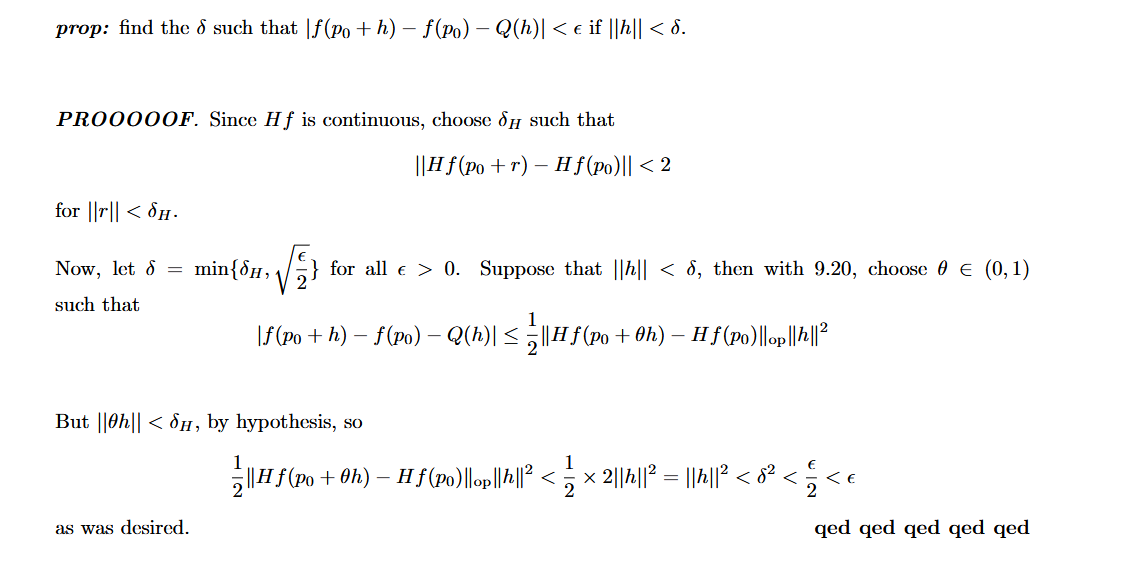
\includegraphics[scale=0.45]{../images/9.21.png}

    \subsubsection{14.8}
    \textbf{Writeup:} Ali\\
\textbf{Solvers:} Ethan, Ryan, Ali\\\\
\textbf{14.8 Theorem} \textit{invariance of volume under reparametrization}
    Let $M$ be a parametrizable set in $\R^N$, and let $\alpha:U\rightarrow M$ and $\beta:V\rightarrow M$ two parametrizations of $M$, where $U,V\subseteq \R^n$ are two open sets. Suppose that $\Phi:U\rightarrow V$ is a diffeomorphism such that $\beta \circ \Phi = \alpha$. Then
        \[ \vol_\alpha(M) = \vol_\beta(M). \]
\begin{proof}
    \[\vol_\alpha(M)=\int_U V(J\alpha)\]
    By definition of $\vol$
    \[\int_U V(J\alpha)=\int_{\Phi^{-1}(V)} V(J(\beta\circ\Phi))\]
    By definition of $\Phi$
    \[\int_{\Phi^{-1}(V)} V(J(\beta\circ\Phi))=\int_{\Phi^{-1}(V)} V((J\beta\circ\Phi)\circ J\Phi)\]
    By application of the multivariate chain rule on $J(\beta\circ\Phi)$
    \[\int_{\Phi^{-1}(V)} V((J\beta\circ\Phi)\circ J\Phi)=\int_{\Phi^{-1}(V)} \sqrt{\det(((J\beta\circ\Phi)\circ J\Phi)^t((J\beta\circ\Phi)\circ J\Phi))}\]
    By the definition of $V$, the volume of a parallelepiped
    \[\int_{\Phi^{-1}(V)} \sqrt{\det(((J\beta\circ\Phi)\circ J\Phi)^t((J\beta\circ\Phi)\circ J\Phi))}=\int_{\Phi^{-1}(V)} \sqrt{\det((J\Phi)^t(J\beta\circ\Phi)^t(J\beta\circ\Phi)(J\Phi))}\]
    By property of transpose $(AB)^t=B^tA^t$ for matrices $A$ and $B$
    \[\int_{\Phi^{-1}(V)} \sqrt{\det((J\Phi)^t(J\beta\circ\Phi)^t(J\beta\circ\Phi)(J\Phi))}=\int_{\Phi^{-1}(V)} \sqrt{\det(J\Phi)^t\det((J\beta\circ\Phi)^t(J\beta\circ\Phi))\det(J\Phi)}\]
    Because $J\Phi$ is a square matrix and by the properties of determinant
    \[\int_{\Phi^{-1}(V)} \sqrt{\det(J\Phi)^t\det((J\beta\circ\Phi)^t(J\beta\circ\Phi))\det(J\Phi)}=\int_{\Phi^{-1}(V)} \sqrt{\det((J\beta\circ\Phi)^t(J\beta\circ\Phi))\det(J\Phi)^2}\]
    Because $\det A^t=\det A$ for any square matrix $A$
    \[\int_{\Phi^{-1}(V)} \sqrt{\det((J\beta\circ\Phi)^t(J\beta\circ\Phi))\det(J\Phi)^2}=\int_{\Phi^{-1}(V)} \sqrt{\det((J\beta\circ\Phi)^t(J\beta\circ\Phi))}\cdot|\det J\Phi|\]
    Because $\sqrt{x^2}=|x|$
    \[\int_{\Phi^{-1}(V)} \sqrt{\det((J\beta\circ\Phi)^t(J\beta\circ\Phi))}\cdot|\det J\Phi|=\int_{\Phi^{-1}(V)} V(J\beta\circ\Phi)\cdot|\det J\Phi|\]
    By the definition of $V$
    \[\int_{\Phi^{-1}(V)} V(J\beta\circ\Phi)\cdot|\det J\Phi|=\int_{\Phi^{-1}(V)} (V(J\beta)\circ\Phi)\cdot|\det J\Phi|\]
    Because $V(J\beta\circ\Phi)=V\circ J\beta\circ\Phi=V(J\beta)\circ\Phi$
    
    \[\int_{\Phi^{-1}(V)} (V(J\beta)\circ\Phi)\cdot|\det J\Phi|=\int_V V(J\beta)\]
    By the Change of Variables Theorem from Unit 13\\\\
    Finally, we have shown that \[\vol_\alpha(M)=\int_UV(J\alpha)=\int_VV(J\beta)=\vol_\beta(M)\]
    As needed.
\end{proof}






    \section{Original Work}
    \begin{thm}
        Let \((X, d)\) be a separable metric space. Then \(A \subseteq X\) is separable with respect to the metric \(d\).
    \end{thm}
    \begin{proof}
        Since \(X\) is separable, it is pre-totally bounded. We will show that a metric subspace \(A\) is separable by showing that it is pre-totally bounded.

        Let \(\varepsilon > 0\). Since \(X\) is pre-totally bounded, there exists a finite collection of open balls \(\{ B(x_i, \frac{\varepsilon}{2})\}_{i\leq n}\) that covers \(X\). We define the desired collection of open balls in \(A\) with the following method:

        If \(B(x_i, \frac{\varepsilon}{2})\) contains some element \(a_i \in A\), we add \(B_A(a_i, \varepsilon)\) to the collection. Notice for \(a \in B(x_i, \frac{\varepsilon}{2}) \cap A\),
        \[
            d(a,a_i) \leq d(x, a) + d(x,a_i) < \frac{\varepsilon}{2} + \frac{\varepsilon}{2} = \varepsilon \text{,} 
        \]
        which implies that \(B(x_i, \frac{\varepsilon}{2}) \subseteq B_A(a_i, \varepsilon)\).

        Continuing on, the number of open balls in this collection is at most the number of open balls in the original collection in \(X\), so \(\{B_A(a_i, \varepsilon)\}\) is finite.

        It remains to show that the collection covers \(A\). Let \(a \in A\). Then \(a \in B(x_i, \frac{\varepsilon}{2})\) for some \(i\). It follows that \(a \in B(x_i,\frac{\varepsilon}{2})\cap A \subseteq B_A(a_i, \varepsilon)\). Thus \(A\) is covered by this collection, so \(A\) is pre-totally bounded.

        Thus we can conclude that \(A\) is separable.

    \end{proof}

    \begin{thm}
        Let \(X,Y\) be metric spaces let and \(f \colon C \to X\) be a continuous function. If \(A \subseteq X\) is seperable, then \(f(A)\) is seperable.
    \end{thm}
    \begin{proof}
        Define \(d_X\) and \(d_Y\) to be metrics on \(X\) and \(Y\) respectively. Suppose that \(A\) is seperable. We will show that \(f(A)\) is seperable by equivalently showing that it is pre-totally bounded.

        Let \(\varepsilon > 0\). By the continuity of \(f\), for every \(a \in A\), there exists \(\delta > 0\) such that for all \(x \in A\), \(d_X(x, a) < \delta \implies d_Y(f(x), f(a)) < \varepsilon\). Keep this value of \(\delta\).

        Since \(A\) is seperable, \(A\) is pre-totally bounded. By definition, \(A\) is covered by a countable subcover \(\{B_X(a_i, \delta)\}_{i\in\mathbb{N}}\).

        Consider the countable collection \(\{B_Y(f(a_i), \varepsilon)\}_{i\in\mathbb{N}}\). We will show that this collection covers \(f(A)\). Let \(y \in f(A)\). Then \(y = f(x)\) for some \(x \in A \subseteq \{B_X(a_i, \delta)\}_{i\in\mathbb{N}}\). This implies that \(x\) is an some open ball \(B_X(a_k, \delta) \implies d_X(x, a_k) < \delta\). By the continuity of \(f\), this implies that \(d_Y(y, f(a_k)) = d_Y(f(x), f(a_k)) < \varepsilon \implies y \in B_Y(f(a_k), \varepsilon) \subseteq \{B_Y(f(a_i), \varepsilon)\}_{i\in\mathbb{N}}\).

        We see that \(f(A)\) is pre-totally bounded, which implies that \(f(A)\) is seperable.
        
    \end{proof}

    \begin{lemma}
        \(\forall x \in X\), \(r > 0\), \(\cl{B}(0, 1) \simeq \cl{B}(x, r)\).
    \end{lemma}
    \begin{proof}
        Let \(x \in X\), \(r >0\). Define the homeomorphism \(f: \cl{B}(0, 1) \to \cl{B}(x, r)\) by
        \[
            f(y) = ry + x
        \]
        First, we will show continuity. Let \(p \in \cl{B}(0,1)\). Let \(\varepsilon > 0\). Let \(\delta = \frac{\varepsilon}{|r|}\). Let \(y \in \cl{B}(0,1)\) such that \(\|y - p\| < \delta\). Then
        \[
            \|f(y) - f(p)\| = \|ry-rp\| = |r|\|y-p\| < \varepsilon
        \]
        We can show that \(f\) is bijective by showing it has a left and right inverse.
        
        Let \(f^{-1}(z) = \frac{1}{r}(z - x)\). Notice that
        \[
            f^{-1}(f(y)) = \frac{1}{r}(f(y) - x) = y
        \]
        and
        \[
            f(f^{-1} (z)) = rf^{-1} (z) - x = z
        \]
        Thus \(f\) is bijective and its inverse is given by \(f^{-1}\), which is continuous, which shows that \(f\) is a homeomorphism.
        \smallbreak
    \end{proof}

    \begin{prop}
        Let \(X\) be a normed vector space. Then \(\cl{B}(0, 1)\) is compact if and only if \(X\) has a compact exhaustion.
    \end{prop}
    \begin{proof}
        Suppose that the closed unit ball is compact. Then we can construct the compact exhaustion \(K_n = \cl{B}(\vec{0}, n)\). These sets are compact because compactness is preserved by the homeomorphism in the lemma. Notice that \((K_n)^\circ \subseteq K_{n+1}\), as
        \[
            x \in (K_n)^\circ \implies \|x\| < n \leq n+1 \implies x \in K_{n+1}
        \]
        Trivally, \(\bigcup_{i=1}^{\infty} K_i \subseteq X\). Now, let \(x \in X\). Then there exists \(j \in \mathbb{N}\) such that \(\|x\| \leq j \implies x \in K_j \subseteq \bigcup_{i=1}^{\infty} K_i\). Thus \(X = \bigcup_{i=1}^{\infty} K_i\), so \(X\) has a compact exhaustion.

        Conversely, assume that \(X\) has a compact exhaustion \((K_n)_{n\geq 1}\). Take the first non-empty set \(K_j\). Since \(K_j \subseteq (K_{j+1})^\circ\), then for \(v \in K_j\), there exists an open ball such that \(B(v, \varepsilon) \subseteq (K_{j+1})^\circ\). It follows that \(\cl{B}(v, \varepsilon) \subseteq K_{j+1}\). By the lemma, it follows that \(\cl{B}(v, \varepsilon) \simeq \cl{B}(0, 1)\), which implies that \(\cl{B}(0,1)\) is compact.
        \smallbreak
    \end{proof}

    \begin{cor}
        Let \(X\) be a normed vector space. Then \(X\) has a compact exhaustion if and only if \(X\) is finite dimensional.
    \end{cor}

    \begin{defn}
        Let \(p > 0\). For \(x = (x_1, ..., x_n) \in \mathbb{R}^n\), the \textbf{p-norm} of \(x\) is defined by
        \[
            \|x\| _p = \sqrt[p]{\sum_{i=1}^n |x_i|^p}
        \]
    \end{defn}

    \begin{prop}
        Equip \(\mathbb{R}^n\) with any norm \(\|\cdot\| _a\). Let \(f : \mathbb{R}^n \to \mathbb{R}\) be a function given by \(f(x) = \|x\|\), for any norm \(\|\cdot\|\) on \(\mathbb{R}^n\). Then \(f\) is not differentiable at \(x=0\).
    \end{prop}
    \begin{proof}
        Suppose for contradiction that \(f\) is differentiable at \(x=0\). Then it has a linear approximation at \(0\). That is, for some \(L \in B(\mathbb{R}^n, \mathbb{R})\),
        \[
            \lim_{h \to 0} \frac{f(h) - f(0) - L(h)}{\|h\| _a} = 0 \implies \lim_{h \to 0} \frac{\|h\| - L(h)}{\|h\| _a} = 0
        \]
        Since norms are equivalent in \(\mathbb{R}^n\), there exists an \(N > 0\) such that
        \[
            N\|h\| _a \leq \|h\| \text{, for all } h \in \mathbb{R}^n
        \]
        Using the limit definition, for \(h \in \mathbb{R}^n\) such that \(\|h\|\) is smaller than some \(\delta\),
        \[
            \left\vert \|h\| - L(h) \right\vert < N\|h\| _a
        \]
        We can also take the negative of this \(h\) and use the linearity of \(L\) to see that
        \[
            \left\vert \|h\| + L(h) \right\vert < N\|h\| _a
        \]
        We see that for all \(h\), \(\|h\| <\delta\),
        \[
            \|h\| = \frac{1}{2} \|(h + L(h)) + (h - L(h))\| \leq \frac{1}{2} \left(\|h + L(h)\| + \|h - L(h)\|\right) < \frac{1}{2} (N \|h\| _a + N \|h\| _a)
        \]
        \[
            \implies \|h\| < N\|h\| _a
        \]
        which is a contradiction.
        \smallbreak
    \end{proof}

    \begin{thm}
        (Fubini's Theorem) Let \(E \subseteq \mathbb{R}^c, F \subseteq \mathbb{R}^d\) be two measurable sets. Let \(f: E \times F \to \mathbb{R}\) be an integrable function such that the \(x\)-slice \(f(x, \cdot)\) is integrable for all \(x \in E\). Define \(\int _F f : E \to \mathbb{R}\) by \((\int _F f)(x) = \int _F f(x, \cdot)\). Then
        \[
            \int _{E \times F} f = \int _E \int _F f
        \]
    \end{thm}
    \begin{proof}
        Let \(P,Q\) be partitions for \(E\) and \(F\) respectively. Consider the subbox \(P_i\) of \(P\). For each subbox \(Q_j\) in \(Q\), define \(M_{ij} = \sup \{ f(x,y) : (x,y) \in P_i \times Q_j \}\). For any \(x_0 \in P_i\), we have
        \[
            \int _F f(x_0, \cdot) \leq U(f(x_0, \cdot), Q) = \sum_{j=1}^{m} \sup \{ f(x_0, y) : y \in Q_j\} \vol (Q_j) \leq \sum_{j=1}^{m} M_{ij} \vol(Q_j)
        \]
        \[
            \implies \sup \left\{ \int _F f(x, \cdot) : x \in P_i \right\} \leq \sum_{j=1}^{m} M_{ij} \vol(Q_j)
        \]
        \[
            \implies U\left( \int _F f, P \right) \leq \sum_{i=1}^{n} \sum_{j=1}^{m} M_{ij} \vol(Q_j) \vol(P_i) = U(f, (P,Q))
        \]
        \[
            \implies \int _E \int _F f \leq U(f)
        \]
        By an analogous argument, we can additionally show that \(\int _E \int _F f \geq L(f)\). Thus
        \[
            L(f) \leq \int _E \int _F f \leq U(f)
        \]
        and since \(L(f) = U(f) = \int _{E \times F} f\), we can conclude that
        \[
            \int _{E \times F} f = \int _E \int _F f.
        \]
    \end{proof}

    \begin{prop}
        \textbf{Exact equations.} Let \(M,N : \mathbb{R}^2 \to \mathbb{R}\) be totally differentiable functions. Then there exists a twice differentiable function \(F: \mathbb{R}^2 \to \mathbb{R}\) such that \(\dfrac{\partial F}{\partial x} = M\) and \(\dfrac{\partial F}{\partial y} = N\) if and only if \(\dfrac{\partial M}{\partial y} = \dfrac{\partial N}{\partial x}\).
    \end{prop}
    \begin{proof}
        Suppose that such \(F\) does indeed exist and is \(C^2\). By Clairaut's theorem we have
        \[
            \frac{\partial M}{\partial y} = \frac{\partial^2 F}{\partial y \partial x} = \frac{\partial^2 F}{\partial x \partial y} = \frac{\partial N}{\partial x}
        \]
        Conversely, suppose that \(\dfrac{\partial M}{\partial y} = \dfrac{\partial N}{\partial x}\). We define \(\int f\ dx\) to be the antiderivative of \(f(.,y)\) with additional constant \(C=0\), and likewise for \(\int f\ dy\). Since \(N,M\) are continuous, they are integrable with respect to both \(x\) and \(y\). Furthermore, their antiderivative and partial derivatives are integrable because they are continuous. Let \(F\) be defined by
        \[
            F(x,y) = \frac{1}{2}\int M(x,y)\ dx + \frac{1}{2}\int N(x,y)\ dy
        \]
        Taking the partial derivative with respect to \(x\), with the application of Feynmann's technique we see that
        \begin{align*}
            \frac{\partial F}{\partial x} (x,y) &= \frac{1}{2}M(x,y) + \frac{1}{2}\int \frac{\partial N}{\partial x} (x,y)\ dy \\
            &= \frac{1}{2}M(x,y) + \frac{1}{2}\int \frac{\partial M}{\partial y} (x,y)\ dy \\
            &= \frac{1}{2}M(x,y) + \frac{1}{2}M(x,y) \\
            &= M(x,y)
        \end{align*}
        Since \(F\) is symmetric, taking the partial derivative with respect to \(y\) will similarly give us \(\dfrac{\partial F}{\partial y} (x,y) = N(x,y)\), and the proof is complete.
        \smallbreak
    \end{proof}
    \begin{cor}
        Suppose we have a differential equation of the form
        \[
            M(x,y) + N(x,y) \frac{dy}{dx} = 0
        \]
        where \(M,N: \mathbb{R}^2 \to \mathbb{R}\) are \(C^1\) functions in terms of \(x\) and \(y\), \(N \neq 0\), and \(\dfrac{\partial M}{\partial y} = \dfrac{\partial N}{\partial x}\). Then this differential equation has a solution.
    \end{cor}
    \begin{proof}
        By the proposition above, we have that there exists some \(C^2\) function \(F : \mathbb{R}^2 \to \mathbb{R}\) with \(\frac{\partial F}{\partial x} = M\) and \(\frac{\partial F}{\partial y} = N \neq 0\). In particular, for some \(x_0,y_0 \in \mathbb{R}\),
        \[
            \frac{\partial F}{\partial y}(x_0, y_0) \neq 0.
        \]
        Let \(C\) be an arbitrary constant, and set \(F(x,y) = C\). By the Implicit Function Theorem, we have that there exists an open set \(U \subseteq \mathbb{R}\) containing \(x_0\) and a function \(\Psi : U \to \mathbb{R}\) so that
        \[
            F(x, \Psi (x)) = C.
        \]
        We claim that a solution to the differential equation is given by \(\Psi\). We see that by taking the derivative of the equation above, we immediately get the original differential equation:
        \[
            M(x, \Psi (x)) + N(x, \Psi (x))\Psi '(x) = 0.
        \]
    \end{proof}
    It may seem tricky to find the \(\Psi\) function, but the work involved amounts to isolating \(y\) in the equation \(F(x,y) = C\), which we will illustrate with the following example.
    \begin{example}
        Find the solution to the differential equation
        \[
            x \dfrac{dy}{dx} + y = 2xe^x + 6x^2.
        \]
        Let \(M(x,y) = 2xe^x + 6x^2 - y\), \(N(x,y) = -x\). We see that
        \[
            \frac{\partial M}{\partial y} (x,y) = -1 = \frac{\partial N}{\partial x} (x,y)
        \]
        By the proposition above, we can find a function \(F : \mathbb{R}^2 \to \mathbb{R}\) so that
        \[
            \frac{\partial F}{\partial x}(x,y) = M(x,y) \text{ and } \frac{\partial F}{\partial y}(x,y) = N(x,y).
        \]
        In particular, by following the explicit formula, we have
        \[
            F(x,y) = 2xe^x - 2e^x + 2x^3 - xy.
        \]
        Set \(2xe^x - 2e^x + 2x^3 - xy = C\), for some constant \(C \in \mathbb{R}\). We claim the solution to the differential equation is \(y = 2e^x - \frac{2}{x}e^x + 2x^2 - \frac{C}{x}\). Indeed, we have that
        \[
            \frac{dy}{dx} = 2e^x + \frac{2}{x^2}e^x - \frac{2}{x}e^x + 4x + \frac{C}{x^2}
        \]
        so
        \[
            x \frac{dy}{dx} + y = x\left( 2e^x + \frac{2}{x^2}e^x - \frac{2}{x}e^x + 4x + \frac{C}{x^2} \right) + 2e^x - \frac{2}{x}e^x + 2x^2 - \frac{C}{x} = 2xe^x + 6x^2
        \]
        as desired.
    \end{example}
    We can generalize this result to multiple variables:
    \begin{thm}
        Let \(N_1, ..., N_n: \mathbb{R}^n \to \mathbb{R}^m\) be differentiable functions. Then there exists a twice differentiable function \(F: \mathbb{R}^n \to \mathbb{R}^m\) such that \(\frac{\partial F}{\partial x_i} = N_i\) if and only if \(\frac{\partial N_i}{\partial x_j} = \frac{\partial N_j}{\partial x_i}\) for all \(i,j \in \{ 1, ..., n \}\).
    \end{thm}
    \begin{proof}
        Suppose such \(F\) does exist. For each \(i,j\), we can apply Clairaut's Theorem to each component function of \(N_i, N_j\) to see that
        \[
            \frac{\partial N_i}{\partial x_j} = \frac{\partial F}{\partial x_j \partial x_i} = \frac{\partial F}{\partial x_i \partial x_j} = \frac{\partial N_j}{\partial x_i}.
        \]
        Conversely, suppose that \(\frac{\partial N_i}{\partial x_j} = \frac{\partial N_j}{\partial x_i}\) for all \(i,j \in \{ 1, ..., n \}\). Similar to the smaller case, define
        \[
            F(x_1, ..., x_n) = \frac{1}{n}\sum_{i=1}^{n} \int N_i (x_1, ..., x_n)\ dx_i
        \]
        For \(k = 1,2,...,n\), we see that
        \begin{align*}
            \frac{\partial F}{\partial x_k} &= \frac{1}{n}\sum_{i=1}^{n} \frac{\partial N_i}{\partial x_k}(x_1, ..., x_n) \ dx_i \\
            &= \frac{1}{n}\left(N_k(x_1, ..., x_n) + \sum_{i\neq k} \int \frac{\partial N_i}{\partial x_k} \ dx_i \right) \\
            &=  \frac{1}{n} \left( N_k(x_1, ..., x_n) + \sum_{i\neq k} \int \frac{\partial N_k}{\partial x_i} (x_1, ..., x_n)\ dx_i \right) \\
            &= \frac{1}{n} \left( N_k(x_1, ..., x_n) + \sum_{i\neq k} N_k(x_1, ..., x_n) \right) \\
            &= \frac{1}{n}\left( n N_k(x_1, ..., x_n) \right) \\
            &= N_k(x_1, ..., x_n)
        \end{align*}
    \end{proof}
    We can use this notion to define a multivariate antiderivative as follows:
    \begin{defn}
        Let \(f: U \subseteq \mathbb{R}^n \to \mathbb{R}^{nm}\) be a function of the form \(f(x_1, ..., x_n) = (f_1(x_1, ..., x_n), ..., f_n(x_1, ..., x_n))\), where \(U\) is open and each \(f_i: U \to \mathbb{R}^m\) are differentiable functions. An \textbf{antiderivative} of \(f\), if it exists, is a function \(F: U \subseteq \mathbb{R}^n \to \mathbb{R}^m\) such that \(\frac{\partial F}{\partial x_i} = f_i\) for all \(i\).
    \end{defn}
    We can also define repeated antiderivatives recursively.
    \begin{defn}
        Let \(k \in \mathbb{N}\), \(f: \mathbb{R}^n \to \mathbb{R}^{n^km}\). The \(k\)th antiderivative of \(f\) is
        \begin{itemize}
            \item The antiderivative of \(f\) if \(k = 1\) (in the sense of the definition above),
            \item The antiderivative of the \(k-1\)th antiderivative of \(f\) if \(k > 1\).
        \end{itemize}
    \end{defn}
    \begin{example}
        Let \(f: \mathbb{R}^3 \to \mathbb{R}^3\) be defined by
        \[
            f(x,y,z) = (y^2 \sin z,2xy \sin z,xy^2 \cos z).
        \]
        We first verify that \(f\) has an antiderivative. We compare the required partial derivatives:
        \begin{align*}
            \frac{\partial f_x}{\partial y} (x,y,z) &= 2y\sin z \\
            \frac{\partial f_y}{\partial x} (x,y,z) &= 2y\sin z \\
            \frac{\partial f_x}{\partial z} (x,y,z) &= y^2 \cos z \\
            \frac{\partial f_z}{\partial x} (x,y,z) &= y^2 \cos z \\
            \frac{\partial f_y}{\partial z} (x,y,z) &= 2xy \cos z \\
            \frac{\partial f_z}{\partial y} (x,y,z) &= 2xy \cos z \\
        \end{align*}
        Since the pairs match, we confirm that the antiderivative of \(f\) does indeed exist and is given by
        \[
            F(x,y,z) = \frac{1}{3}\left(\int y^2 \sin z\ dx + \int 2xy \sin z\ dy + \int xy^2 \cos z\ dz\right) = xy^2 \sin z
        \]
    \end{example}
    A motivation for defining antiderivatives in this way is to be able to express higher order derivatives in a more condensed and understandable way, as we will see below. First, we define a way to transform functions between arbitrary finite dimensional vector spaces over \(\mathbb{R}\) into functions between \(\mathbb{R}^n\) and \(\mathbb{R}^m\).
    \begin{defn}
        Let \(V,W\) be finite dimensional vector spaces with dimensions \(n,m\) respectively and let \(f : V \to W\) be a function. Let \(\alpha ,\beta \) be ordered bases for \(V,W\), and let \(\phi _\alpha : V \to \mathbb{R}^n\) be the standard coordinate isomorphism to \(\mathbb{R}^n\) corresponding to \(\alpha\), and define \(\phi _\beta\) similarly. A \textbf{coordinate representation} for \(f\) with respect to \(\alpha\) and \(\beta\) is the function \(\hat{f}: \mathbb{R}^n \to \mathbb{R}^m\) defined by
        \[
            \hat{f} = \phi _\beta \circ f \circ \phi_\alpha^{-1}.
        \]
    \end{defn}
    \begin{thm}
        If \(F: U \subseteq \mathbb{R}^n \to \mathbb{R}^m\) is the antiderivative of \(f = (f_1, ..., f_n) : \mathbb{R}^n \to \mathbb{R}^{nm}\), then 
        \[
            JF(p) = \begin{pmatrix}
                f_1(p) \\
                \vdots \\
                f_n(p) \\
            \end{pmatrix}^t
        \]
        for all \(p \in U\).
    \end{thm}
    \begin{proof}
        Let \(F = (F_1, ..., F_m)\), where \(F_i : \mathbb{R}^n \to \mathbb{R}\) are functions. As well, write
        \[
            f = (f_1, ..., f_n)
        \]
        where \(f_i = (f_{i1} , ..., f_{in})\). Then note that
        \[
            (JF(p))_{ij} = \frac{\partial F_i}{\partial x_j}(p)
        \]
        but since \(F\) is the antiderivative of \(f\), we know that \(\frac{\partial F}{\partial x_j} = f_j\), so
        \[
            \frac{\partial F_i}{\partial x_j}(p) = f_{ji} = \begin{pmatrix}
                f_1(p) & \cdots & f_n(p) \\
            \end{pmatrix}_{ji} = \begin{pmatrix}
                f_1(p) \\
                \vdots \\
                f_n(p) \\
            \end{pmatrix}^t_{ij}.
        \]
    \end{proof}
    It follows that \(f\) is the coordinate representation for \((JF)^t\) with respect to the standard bases of \(\mathbb{R}^n\) and \(M_{n\times m}(\mathbb{R})\). We call such a function to be the \textbf{function representation} of \(JF\) or \(F'\). This concept may not be too useful when only working with first derivatives, but quickly becomes enticing when used for higher order derivatives.
    \begin{thm}
        Let \(F: \mathbb{R}^n \to \mathbb{R}^m\) be a smooth function, and let \(f: \mathbb{R}^n \to \mathbb{R}^{n^k m}\) be the function representation of \(J^k F\). Then the function representation of \(f'\) is also the function representation of \(J^{k+1} F\).
    \end{thm}
    \begin{proof}
        We denote \(f = (f_1, ..., f_{n^k m})\), where \(f_i : \mathbb{R}^n \to \mathbb{R}\) are functions. Let \(g\) be the function representation of \(f'\). Write \(g = (g_1, ..., g_n)\), where \(g_i : \mathbb{R}^n \to \mathbb{R}^{n^{k+1}m}\) are functions. Then
        \[
            Jf = \begin{pmatrix}
                 g_1 \\
                 \vdots \\
                 g_n \\
            \end{pmatrix}^t.
        \]
        But since \(f\) is the function representation of \(J^k F\),
        \[
            J^k F = \begin{pmatrix}
                 f_1 \\
                 \vdots \\
                 f_n \\
            \end{pmatrix}^t.
        \]
        We take the Jacobian of both sides to obtain that
        \[
            J^{k+1} F = \begin{pmatrix}
                \frac{\partial f_{1}}{\partial x_1} & \cdots & \frac{\partial f_{1}}{\partial x_n} \\
                \vdots & \ddots & \vdots \\
                \frac{\partial f_{n^{k}m}}{\partial x_1} & \cdots & \frac{\partial f_{n^k m}}{\partial x_n}
            \end{pmatrix}
        \]
    \end{proof}

    Next, we prepare some definitions and propositions to help us prove the main result.
    \begin{defn}
        A \textbf{monomial} in \(n\) variables is a function \(m : \mathbb{R}^n \to \mathbb{R}\) of the form \(m(x_1, ..., x_n) = x_1^{i_1}\cdots x_n^{i_n}\), where \(i_1, ..., i_n \geq 0\). The degree of a monomial is \(\mathrm{deg} (m) = i_1 + \cdots + i_n\). A \textbf{polynomial} is a linear combination of monomials, and its degree is defined to be the degree of the monomial with the highest degree. Additionally, we define a \textbf{\(k\)-polynomial} to be a function \(f: \mathbb{R}^n \to \mathbb{R}^k\) such that each component is a polynomial in \(n\) variables. Likewise, its degree is defined to be the degree of the highest degree component. Note that using this definition, a polynomial in the sense of the above definition is considered a 1-polynomial.
    \end{defn}
    \begin{prop}
        Let \(f: \mathbb{R}^n \to \mathbb{R}^k\) be a \(k\)-polynomial in \(n\) variables. Then the characteristic function of \(Jf\) is a \(nk\)-polynomial in \(n\) variables.
    \end{prop}
    \begin{proof}
        Let \(g: \mathbb{R}^n \to \mathbb{R}^{nk}\) be the characteristic function of \(Jf\). By Theorem 4.15, we know that each component function of \(g\) is a partial derivative of some component function of \(f\). Denote this component as \(f_i\). We claim that \(\frac{\partial f_i}{\partial x_j}\) is a polynomial.
    \end{proof}

    % \begin{prop}
    %     All polynomials in \(n\) variables are infinitely differentiable.
    % \end{prop}
    % \begin{proof}
    %     Let \(f : \mathbb{R}^n \to \mathbb{R}\) be a polynomial. It suffices to show 
    % \end{proof}

    \begin{lemma}
        Let \(g : \mathbb{R}^n \to \mathbb{R}\) be a monomial in \(n\) variables. For each \(i \in \{1, ..., n\}\), there exists \(k_i \in \mathbb{N}\) such that \(\dfrac{\partial ^{k_i} g}{\partial x_i ^{k_i}} = 0\).
    \end{lemma}
    \begin{proof}
        Fix \(p = (p_1, ..., p_n) \in \mathbb{R}^n\). Let \(i \in \{1, ..., n\}\). Define a \(g_i : \mathbb{R} \to \mathbb{R}\) by
        \[
            g_i(x) = g(p_1, ..., p_{i-1}, x, ..., p_n) = p_1^{d_1}\cdots p_{i-1}^{d_{i-1}} p_{i+1}^{d_{i+1}} \cdots x^{d_i}.
        \]
        This is a monomial in 1 variable of degree \(d_i\). Thus \(g_i^{(d_i + 1)} = 0\).

        Notice that
        \[
            \frac{\partial g}{\partial x_i} (p) = \lim_{t \to 0} \frac{g(p+tx_i) - g(p)}{t} = \lim_{t \to 0} \frac{g_i(p_i + t) - g_i(p_i)}{t} = g_i'(p_i)
        \]
        We can observe that this pattern continues for all \(i\)th partial derivatives, so we can conclude that
        \[
            \dfrac{\partial ^{d_i + 1} g}{\partial x_i ^{d_i + 1}}(p) = g_i^{(d_i + 1)}(p_i) = 0
        \]
        which was what we wanted.
        \smallbreak
    \end{proof}
    
    Now, we can prove the main result we sought out to prove.
    \begin{thm}
        Let \(f : \mathbb{R}^n \to \mathbb{R}\) be a polynomial in \(n\) variables. There exists \(k \in \mathbb{N}\) such that \(f^{(k)} = 0\). As well, if \(f\) is a function such that \(f^{(k)} = 0\) for some \(k \in \mathbb{N}\), then \(f\) is necessarily a polynomial.
    \end{thm}
    \begin{proof}
        Let \(d_m\) denote the degree of \(f^{(m)}\). We claim that if \(d_m > 0\), then \(d_{m+1} < d_m\). Let \(g_m\) be the characteristic function of 
    \end{proof}
    \subsection{Precompactness}
    We know that compactness can play a big role in proving results, such as the existence of partitions of unity. Here, we look into a slightly weaker version of compactness and see what results can be proved with it.
    \begin{defn}
        A metric space \(X\) is \textit{precompact} if any open cover permits a \textit{countable} subcover.
    \end{defn}
    While it can be cumbersome to directly find examples of precompact metric spaces, we can show that precompactness is equivalent to certain metric space properties, and thus show that all metric spaces with those properties are also precompact.
    \begin{prop}
        A metric space is precompact if and only if it is separable.
    \end{prop}
    \begin{proof}
        Let \(X\) be a metric space. Suppose that \(X\) is precompact. For \(n \in \mathbb{N}\), let \(U_n = \{ B\left( x_{ni}, \frac{1}{n} \right) \}_{i \in I}\) be an open cover of \(X\), and suppose without loss of generality that \(U_n\) is countable. It follows that \(U = \bigcup_{n=1}^{\infty} U_n\) is countable as well. Let \(C = \{ x_{ni} \}_{i \in I}\) be the collection of all the open ball centers in \(U\). This set is countable, so it only remains to show that \(C\) is dense in \(X\). Let \(x \in X\), \(\varepsilon > 0\). Take \(n\) such that \(\frac{1}{n} < \varepsilon\). Then \(x\) is contained in some open ball \(B(x_i , \frac{1}{n})\). But this implies that \(x_i \in B(x, \varepsilon)\), so \(C\) is dense. Thus \(X\) is separable.

        Conversely, suppose that \(X\) is separable. Let \(\{ U_i \} _{i \in I}\) be an open cover for \(X\). Let \(C \subseteq X\) be a separable subset of \(X\) and write it as \(C = \{ q_1, q_2, ... \}\). We construct the countable subcover \(U\) as follows. For all \(n,k \in \mathbb{N}\), consider the open ball \(B(q_n, \frac{1}{k})\). For each of these balls, if there exists an open set \(U_{nk}\) inside the cover such that \(B(q_n, \frac{1}{k}) \subseteq U_{nk}\), we include \(U_{nk}\) inside the subcover. Notice that \(U\) is countable by construction.

        Let \(x \in X\). There is some open set \(U_i\), not necessarily in \(U\) that contains \(x\). Take the open ball \(B(x, \delta) \subseteq U_i\). By the separability of \(X\), there exists some \(q_n \in C\) so that \(q_n \in B( x, \frac{\delta}{2} )\). Let \(k \in \mathbb{N}\) such that \(\frac{1}{k} < \frac{\delta}{2}\) and consider another open ball \(B(q_n, \frac{1}{k}) \subseteq B(x, \delta)\). We are guaranteed that \(U_{nk}\) exists, because \(B(q_n, \frac{1}{k}) \subseteq U_i\), so \(B(q_n, \frac{1}{k})\) of at least one set in the open cover. Thus \(x \in U_{nk} \in U\), so \(U\) is indeed a countable open cover so \(X\) is precompact.
    \end{proof}
    \begin{cor}
        Every subset of a precompact metric space is also precompact.
    \end{cor}
    \begin{proof}
        We know that precompactness is equivalent to separability, and we also know that any subset of a separable metric space is also separable, and thus precompact.
    \end{proof}
    For this section, we focus mainly on \(\mathbb{R}^n\) rather than arbitrary precompact metric spaces.
    \begin{prop}
        Every set with a compact exhaustion is precompact.
    \end{prop}
    \begin{proof}
        Let \(A\) be a set with a compact exhaustion \(K_n\). Let \(\{ U_i \} _{i \in I}\) be an open cover of \(A\). Notice that this is also an open cover for each \(K_n\), which induces a finite subcover \(\mathcal{U}_n\) for each compact set. We take the countable union of these sets and claim that is the desired countable subcover.

        Let \(x \in A\). Then \(x\) is contained in some \(K_n\). But this implies that \(x\) is in some open set \(U_i\) such that \(U_i \in \mathcal{U}_n\), so this choice is indeed a countable subcover.
    \end{proof}
    \begin{cor}
        \(\mathbb{R}^n\) is precompact.
    \end{cor}
    \begin{proof}
        This can be seen quickly, as \(\left( \cl{B}(0, n) \right)_{n \in \mathbb{N}}\) is a compact exhaustion of \(\mathbb{R}^n\), so we can apply the proposition above to obtain our conclusion.
    \end{proof}
    \begin{thm}
        Let \(M \subseteq \mathbb{R}^N\) be a manifold. Then \(M\) has a countable atlas.
    \end{thm}
    \begin{proof}
        Let \(\{ (U_i , \varphi _i) \}_{i \in I}\) be an atlas for \(M\). Since \(\{ U_i \}\) constitutes an open cover of \(M\), we can find a countable subcover \(\{ U_{i_n} \}_{n \in \mathbb{N}}\) by the precompactness of \(M\). Then \(\{ (U_{i_n}, \varphi _{i_n}) \}_{n \in \mathbb{N}}\) is still an atlas over \(M\), but is countable, so we are done.
    \end{proof}

\end{document}